\documentclass[twoside, 11pt]{article}

% Any additional packages needed should be included after jmlr2e.
% Note that jmlr2e.sty includes epsfig, amssymb, natbib and graphicx,
% and defines many common macros, such as 'proof' and 'example'.
%
% It also sets the bibliographystyle to plainnat; for more information on
% natbib citation styles, see the natbib documentation, a copy of which
% is archived at http://www.jmlr.org/format/natbib.pdf

\usepackage{jmlr2e}
\usepackage[algo2e,ruled]{algorithm2e}
%\usepackage{natbib,booktabs}
\usepackage{graphicx} % more modern
\usepackage{subfigure}
\usepackage{hyperref,multirow,float}
\usepackage{xspace}
\usepackage{subfigure}
\usepackage{amsmath}
\usepackage{steinmetz}
\usepackage{float}

\usepackage{color}
\usepackage{xcolor}
\usepackage{lastpage}


\jmlrheading{19}{2018}{1-\pageref{LastPage}}{1/15; Revised 4/16}{12/18}{15-020}{Dhruv Mahajan, Nikunj Agrawal, S. Sathiya Keerthi, Sundararajan Sellamanickam and L\'{e}on Bottou}
% Short headings should be running head and authors last names

\ShortHeadings{An efficient distributed learning algorithm}{Mahajan, Agrawal, Keerthi, Sellamanickam and Bottou}
\firstpageno{1}

\newcommand*{\Scale}[2][4]{\scalebox{#1}{\ensuremath{#2}}}%


\begin{document}
\sloppy

\title{An efficient distributed learning algorithm based on effective local functional approximations}

\author{\name Dhruv Mahajan \email dhruvm@fb.com \\
       \addr Facebook AI\\
       Menlo Park, CA 94025, USA
       \AND
       \name Nikunj Agrawal \email nikunj157@gmail.com \\
       \addr Indian Institute of Technology \\
       Dept. of Computer Science \& Engineering \\
       Kanpur, India
       \AND
       \name S. Sathiya Keerthi \email keerthi@microsoft.com \\
       \addr Office Data Science Group\\
       Microsoft\\
       Mountain View, CA 94043, USA
       \AND
       \name Sundararajan Sellamanickam \email ssrajan@microsoft.com \\
       \addr Microsoft Research \\
       Bangalore, India
       \AND
       \name L\'{e}on Bottou \email leon@bottou.org \\
      \addr Facebook AI Research \\
      New York, NY, USA
       }

\editor{Inderjit Dhillon}

\maketitle
\begin{abstract}%   <- trailing '%' for backward compatibility of .sty file
Scalable machine learning over big data is an important problem that is receiving a lot of attention in recent years. On popular distributed environments such as Hadoop running on a cluster of commodity machines, communication costs are substantial and algorithms need to be designed suitably considering those costs.
In this paper we give a novel approach to the distributed training of linear classifiers (involving smooth losses and $L_2$ regularization) that is designed to reduce the total communication costs. At each iteration, the nodes minimize locally formed approximate objective functions; then the resulting minimizers are combined to form a descent direction to move. Our approach gives a lot of freedom in the formation of the approximate objective function as well as in the choice of methods to solve them. The method is shown to have $O(\log(1/\epsilon))$ time convergence. The method can be viewed as an iterative parameter mixing method. A special instantiation yields a parallel stochastic gradient descent method with strong convergence. When communication times between nodes are large, our method is much faster than the Terascale method~\citep{agarwal2011}, which is a state of the art distributed solver based on the statistical query model~\citep{chu2006} that computes function and gradient values in a distributed fashion. We also evaluate against other recent distributed methods and demonstrate superior performance of our method.
\end{abstract}

\begin{keywords}
Distributed learning, Example partitioning, $L_2$ regularization
\end{keywords}


\def\grad{\nabla}
\def\wtilde{\tilde{w}}
\def\Cone{{\cal{C}}^1}
\def\kappap{\kappa^\prime}
\def\Lhat{\hat{L}}
\def\fhat{\hat{f}}
\def\what{\hat{w}}
\def\dhat{\hat{d}}
\def\mysgn{\operatorname{sgn}}
\def\ftilde{\tilde{f}}
\def\khat{\hat{k}}
\def\defs{\stackrel{\text{def}}{=}}
\def\vhat{\hat{v}}

\def\ttilde{\tilde{t}}
\def\that{\hat{t}}
\def\tstar{t^\star}
\newcommand{\yrcite}[1]{\citeyearpar{#1}}
\long\def\comment#1{}

\def\K{{\bf ToDo:~}}

\newcommand{\Kee}[1]{\par\textcolor{violet}{\textbf{Keerthi:} #1}}


%\input{intro}

\section{Introduction}
\label{intro}

In recent years, machine learning over Big Data has become an important problem, not only in web related applications, but also more commonly in other applications, e.g., in the data mining over huge amounts of user logs. The data in such applications are usually collected and stored in a decentralized fashion over a cluster of commodity machines (nodes) where communication times between nodes are significantly large.  Examples of applications involving high communication costs include: Click prediction on advertisement data where the number of examples is huge and features are words which can run in to billions, and Geo distributed data across different countries/continents where cross data-center speeds are extremely slow.
In such a settings, it is natural for the examples to be partitioned over the nodes.

Distributed machine learning algorithms that operate on such data are usually iterative. Each iteration involves some {\em computation} that happens locally in each node. In each iteration, there is also {\em communication} of information between nodes and this is special to the distributed nature of solution. Distributed systems such as those based on the Map-Reduce framework~\citep{Dean2008} involve additional special operations per iteration, such as the loading of data from disk to RAM. Recent frameworks such as Spark~\citep{Zaharia2010} and REEF~\citep{weimer2015} avoid such unnecessary repeated loading of data from disk. Still, communication between nodes in each iteration is unavoidable and, its cost can be substantial when working with Big Data.
Therefore, the development of efficient distributed machine learning algorithms that minimize communication between nodes is an important problem. The key is to come up with algorithms that minimize the number of iterations.

In this paper we consider the distributed batch training of linear classifiers in which: (a) both, the number of examples and the number of features are large; (b) the data matrix is sparse; (c) the examples are partitioned over the nodes; (d) the loss function is convex and differentiable; and, (e) the $L_2$ regularizer is employed. This problem involves the large scale unconstrained minimization of a convex, differentiable objective function $f(w)$ where $w$ is the weight vector.
The minimization is usually performed using an iterative descent method in which an iteration starts from a point $w^r$, computes a direction $d^r$ that satisfies
\begin{equation}
\mbox{{\small\bf sufficient angle of descent:}}\; \phase{-g^r, d^r} \le \theta \label{angle}
\end{equation}
where $g^r=g(w^r)$, $g(w)=\grad f(w)$, $\phase{a,b}$ is the angle between vectors $a$ and $b$, and $0 \le \theta < \pi/2$, and then performs a line search along the direction $d^r$ to find the next point, $w^{r+1}=w^r+t d^r$. Let $w^\star=\arg\min_w f(w)$. A key side contribution of this paper is the proof that, when $f$ is convex and satisfies some additional weak assumptions, the method has global linear rate of convergence ({\it glrc})\footnote{We say a method has {\it glrc} if $\exists$ $0<\delta<1$ such that $(f(w^{r+1})-f(w^\star)) \le \delta (f(w^r)-f(w^\star))\;\forall r$.} and so it finds a point $w^r$ satisfying $f(w^r)-f(w^\star)\le\epsilon$ in $O(log(1/\epsilon))$ iterations. {\it The main theme of this paper is that the flexibility offered by this method with strong convergence properties allows us to build a class of useful distributed learning methods with good computation and communication trade-off capabilities.}

%Let us consider large scale learning in a distributed setting in which examples are partitioned over a number of computing nodes.
Take one of the most effective distributed methods, viz., SQM (Statistical Query Model) \citep{chu2006,agarwal2011}, which is a batch, gradient-based descent method. The gradient is computed in a distributed way with each node computing the gradient component corresponding to its set of examples. This is followed by an aggregation of the components. We are interested in systems in which the communication time between nodes is large relative to the computation time in each node.\footnote{This is the case when feature dimension is huge. Many applications gain performance when the feature space is expanded, say, via feature combinations, explicit expansion of nonlinear kernels etc.} For iterative algorithms such as SQM, the total training time is given by
\begin{equation}
\mbox{Training time} = (T^{cmp} + T^{com})\; T^{iter}
\end{equation}
where $T^{cmp}$ and $T^{com}$ are respectively, the computation time and the communication time per iteration and $T^{iter}$ is the total number of iterations. When $T^{com}$ is large, it is not optimal to work with an algorithm such as SQM that has $T^{cmp}$ small and due to which, $T^{iter}$ is large.
In such a scenario, it is useful to ask: {\bf Q1.} {\it In each iteration, can we do more computation in each node so that the number of iterations and hence the number of communication passes are decreased, thus reducing the total computing time?}
%We will show that this question can be answered positively by using the iterative descent method suitably.

There have been some efforts in the literature to reduce the amount of communication. In one class of such methods, the current $w^r$ is first passed on to all the nodes. Then, each node $p$ forms an approximation $\ftilde_p$ of $f$ using only its examples, followed by several optimization iterations (local passes over its examples) to decrease $\ftilde_p$ and reach a point $w_p$. The $w_p\;\forall p$ are averaged to form the next iterate $w^{r+1}$. One can stop after just one major iteration (going from $r=0$ to $r=1$); such a method is referred to as {\it parameter mixing (PM)}~\citep{mann2009}. Alternatively, one can do many major iterations; such a method is referred to as {\it iterative parameter mixing (IPM)}~\citep{hall2010}. Convergence theory for such methods is inadequate~\citep{mann2009, mcdonald2010}, which prompts us to ask: {\bf Q2.} {\it Is it possible to devise an IPM method that produces $\{w^r\} \rightarrow w^\star$?}

In another class of methods, the dual problem is solved in a distributed fashion~\citep{pechyony2011, yang2013a, yang2013b, jaggi2014}. Let $\alpha_p$ denote the dual vector associated with the examples in node $p$. The basic idea is to optimize $\{\alpha_p\}$ in parallel and then use a combination of the individual directions thus generated to take an overall step. In practice these methods tend to have slow convergence; see~Section~\ref{expts} for details.

%For large scale learning on a single machine, it is now well established that example-wise methods\footnote{These methods update $w$ after scanning each example.} such as stochastic gradient descent (SGD) and its variations~\citep{bottou2010, johnson2013} and dual coordinate ascent~\citep{hsieh2008} are much faster than batch gradient-based methods. However, example-wise methods are inherently sequential. If one employs a method such as SGD as the local optimizer for $\ftilde_p$ in PM/IPM, the result is, in essence, a parallel SGD method. However, convergence theory for such a method is limited, even that requiring a complicated analysis~\citep{zinkevich2010}. Thus, we ask: {\bf Q3.} {\it Can we form a parallel SGD method with strong convergence properties?}

We make a novel and simple use of the iterative descent method mentioned at the beginning of this section to design a distributed algorithm that answers Q1-Q2 positively. The main idea is to use distributed computation for generating a good search direction $d^r$ and not just for forming the gradient as in SQM. At iteration $r$, let us say each node $p$ has the current iterate $w^r$ and the gradient $g^r$. This information can be used together with the examples in the node to form a function $\fhat_p(\cdot)$ that approximates $f(\cdot)$ and satisfies $\grad\fhat_p(w^r)=g^r$. One simple and effective suggestion is:
\begin{equation}
\fhat_p(w)=f_p(w)+(g^r - \nabla f_p(w^r))\cdot(w-w^r)
\label{sugg1}
\end{equation}
where $f_p$ is the part of $f$ that does not depend on examples outside node $p$; the second term in (\ref{sugg1}) can be viewed as an approximation of the objective function part associated with data from the other nodes. In Section~\ref{distr} we give other suggestions for forming $\fhat_p$. Now $\fhat_p$ can be optimized within node $p$ using any method ${\cal M}$ which has {\it glrc}, e.g., Trust region method, L-BFGS, etc. There is no need to optimize $\fhat_p$ fully. We show (see Section~\ref{distr}) that, in a constant number of local passes over examples in node $p$, an approximate minimizer $w_p$ of $\fhat_p$ can be found such that the direction $d_p=w_p-w^r$ satisfies the sufficient angle of descent condition, (\ref{angle}). A convex combination of the set of directions generated in the nodes, $\{d_p\}$ forms the overall direction $d^r$ for iteration $r$. Note that $d^r$ also satisfies (\ref{angle}). The result is an overall distributed method that finds a point $w$ satisfying $f(w)-f(w^\star)\le\epsilon$ in $O(\log (1/\epsilon))$ time. This answers {\bf Q2}.

The method also reduces the number of communication passes over the examples compared with SQM, thus also answering {\bf Q1}. The intuition here is that, if each $\fhat_p$ is a good approximation of $f$, then $d^r$ will be a good global direction for minimizing $f$ at $w^r$, and so the method will move towards $w^\star$ much faster than SQM.

%As one special instantiation of our distributed method, we can use, for the local optimization method ${\cal M}$, any variation of SGD with {\it glrc} (in expectation), e.g., the one in~\citet{johnson2013}. For this case, in a related work we showed that our method has $O(\log (1/\epsilon))$ time convergence in a probabilistic sense~\citep{mahajan2013}. The result is a strongly convergent parallel SGD method, which answers {\bf Q3}. An interesting side observation is that, the single machine version of this instantiation is very close to the variance-reducing SGD method in~\citet{johnson2013}.


%In section~\ref{expts} we demonstrate this via experiments on distributed implementations of the methods using {\it AllReduce} on Hadoop.

%The set up described above can also be used to to devise a method which fills an important gap in the distributed learning literature. Let us first describe this gap before describing our solution. For large scale learning on a single machine, it is now well established that example-wise methods\footnote{These methods update $w$ after scanning each example.} such as stochastic gradient descent (SGD) and its variations~\citep{bottou2010, johnson2013} and dual coordinate ascent~\citep{hsieh2008} are much faster than batch gradient-based methods. However, example-wise methods are inherently sequential. There have been attempts to parallelize them using the following idea: pass the current $w^r$ to all nodes, in each node $p$ apply one or more epochs of SGD on its examples to generate $w_p$, and then average the $w_p$ using a {\it Reduce} operation to form $w^{r+1}$. One can stop such {\it parameter mixing} methods after a single iteration~\citep{zinkevich2010, mann2009} (going from $r=0$ to $r=1$) or do several iterations~\citep{hall2010, mcdonald2010}; however, establishing convergence of such methods is limited as well as hard.

%Let us now briefly describe our solution. Suppose, in our distributed method described earlier, we form $\fhat_p$ using (\ref{sugg1}), use a SGD method as the choice for $\cal{M}$ to minimize $\fhat_p$, and run several epochs of SGD updates over the examples of node $p$, then a $w_p$ can be generated so that $d_p=w_p-w^r$ satisfies (\ref{angle}). Averaging the $d_p$ to generate $d^r$ followed by line search completes an iteration. The resulting instantiation of Algorithm~\ref{GD} has good convergence properties  and is a nice parallelization of SGD. The ability to inject an example-wise method in a batch method is interesting as well as a demonstration of the flexibility offered by our approach to large scale distributed learning. Another interesting observation is that, the single machine version of this instantiation is very close to a recently proposed variance-reducing SGD method~\citep{johnson2013}.

%In summary, the paper makes the following contributions. (1) For convex $f$ we establish {\it glrc} for a general iterative descent method. (2) We propose a distributed learning algorithm that: (a) converges in $O(\log (1/\epsilon))$ time, thus leading to an IPM method with strong convergence; (b) is more efficient than SQM when communication times are high; and (c) flexible in terms of the local optimization method ${\cal M}$ that can be used in the nodes. (3) We give an effective parallelization of SGD with good theoretical support and make connections with a recently proposed variance-reducing SGD method.

In summary, the paper makes the following contributions.
First, for convex $f$ we establish {\it glrc} for a general iterative descent method.
Second, and more important, we propose a distributed learning algorithm that: (a) converges in $O(\log (1/\epsilon))$ time, thus leading to an IPM method with strong convergence; (b) is more efficient than SQM when communication costs are high; and (c) flexible in terms of the local optimization method ${\cal M}$ that can be used in the nodes.

There is also another interesting side contribution associated with our method. It is known that example-wise methods such as stochastic gradient descent (SGD) are inherently sequential and hard to parallelize~\citep{zinkevich2010}. By employing SGD as ${\cal M}$, the local optimizer for $\ftilde_p$ in our method, we obtain a parallel SGD method with good performance as well as strong convergence properties. This contribution is covered in detail in~\citet{mahajan2013}; we give a summarized view in Subsection~\ref{subsec:psgd}.

Experiments (Section~\ref{expts}) validate our theory as well as show the benefits of our method for large dimensional datasets where communication is the bottleneck. We give a discussion on unexplored possibilities for extending our distributed learning method in Section~\ref{disc} and conclude the paper in Section~\ref{conc}.

%We close this section with a brief discussion of works related to this paper.

%\noindent {\bf Related work.} Let us begin with papers related to the general descent method and its convergence.



%\input{convergence}

\section{Basic descent method}
\label{general}

Let $f\in\Cone$, the class of continuously differentiable functions\footnote{It would be interesting future work to extend all the theory developed in this paper to non-differentiable convex functions, using sub-gradients.}, $f$ be convex, and the gradient $g$ satisfy the following assumptions.

\noindent {\bf A1.} $g$ is Lipschitz continuous, i.e., $\exists$ $L>0$ such that
$\|g(w)-g(\wtilde)\| \le L \|w-\wtilde\| \;\;\; \forall \; w, \wtilde$.


\noindent {\bf A2.} $\exists$ $\sigma >0$ such that
$(g(w)-g(\wtilde))\cdot(w-\wtilde) \ge \sigma \|w-\wtilde\|^2  \;\;\; \forall \; w, \wtilde$.

A1 and A2 are essentially second order conditions: if $f$ happens to be twice continuously differentiable, then $L$ and $\sigma$ can be viewed as upper and lower bounds on the eigenvalues of the Hessian of $f$. A convex function $f$ is said to be $\sigma$- strongly convex if $f(w)-\frac{\sigma}{2} \|w\|^2$ is convex. In machine learning, all convex risk functionals in $\Cone$ having the $L_2$ regularization term, $\frac{\lambda}{2} \|w\|^2$ are $\sigma$- strongly convex with $\sigma=\lambda$. It can be shown~\citep{smola2008}
%(see (3.18) there)
that, if $f$ is $\sigma$-strongly convex, then $f$ satisfies assumption A2.

Let $f^r=f(w^r)$, $g^r=g(w^r)$ and $w^{r+1}=w^r+t d^r$. Consider the following standard line search conditions.
\begin{eqnarray}
\mbox{{\small\bf Armijo:}}\; & f^{r+1} \le f^r + \alpha g^r\cdot(w^{r+1}-w^r) \label{ag} \\
\mbox{{\small\bf Wolfe:}}\;  & g^{r+1}\cdot d^r \ge \beta g^r\cdot d^r \label{wolfe}
\end{eqnarray}
where $0<\alpha<\beta<1$.

\begin{algorithm2e}
\caption{Descent method for $f$\label{GD}}
Choose $w^0$\;
\For{$r=0,1 \ldots$}{
1. Exit if $g^r=0$\;
2. Choose a direction $d^r$ satisfying (\ref{angle})\;
3. Do line search to choose $t>0$ so that $w^{r+1}=w^r+td^r$ satisfies the Armijo-Wolfe conditions (\ref{ag}) and (\ref{wolfe})\;
}
\end{algorithm2e}
Let us now consider the general descent method in Algorithm~\ref{GD} for minimizing $f$. The following result shows that the algorithm is well-posed. A proof is given in the appendix B.

%Standard results in optimization~\citep{dennis1996} (see Theorem 6.3.2) can be easily modified to show that there always exists an interval of $t$ values over which (\ref{wolfe}) and (\ref{ag}) hold.


\noindent {\bf Lemma 1.} Suppose $g^r\cdot d^r<0$.
Then $\{ t: $ (\ref{ag}) and (\ref{wolfe}) hold for $w^{r+1}=w^r+td^r\} = [t_\beta,t_\alpha]$, where $0<t_\beta<t_\alpha$, and $t_\beta$, $t_\alpha$ are the unique roots of
\begin{eqnarray}
g(w^r+t_\beta d^r)\cdot d^r = \beta g^r\cdot d^r, \label{tbeta} \\
f(w^r+t_\alpha d^r) = f^r + t_\alpha \alpha g^r\cdot d^r, \;\; t_\alpha>0. \label{talpha}
\end{eqnarray}

%If $\alpha$ is chosen very small, say $\alpha=10^{-4}$ and $\beta$ close to 1, say $0.99$, then this interval becomes large and it is easy to locate a $t$ satisfying the two conditions. (We need to say a bit more here, e.g., give good starting $t$ values and a clean line search algorithm that works and is also efficient. See section~\ref{lsearch} for some ideas for bracketing the minimum in the line search.)

\noindent {\bf Theorem 2.} Let $w^\star=\arg\min_w f(w)$ and $f^\star=f(w^\star)$.\footnote{Assumption A2 implies that $w^\star$ is unique.} Then $\{w^r\}\rightarrow w^\star$. Also, we have {\it glrc}, i.e., $\exists$ $\delta$ satisfying $0<\delta<1$ such that
$(f^{r+1} - f^\star) \le \delta\, (f^r-f^\star) \; \forall \; r\ge 0$,
and, $f^r-f^\star\le\epsilon$ is reached after at most
$\frac{\log ((f^0-f^\star)/\epsilon)}{\log(1/\delta)}$
iterations. An upper bound on $\delta$ is $(1 - 2\alpha(1-\beta)\frac{\sigma^2}{L^2} \cos^2\theta)$.

A proof of Theorem 2 is given in the appendix B. If one is interested only in proving convergence, it is easy to establish under the assumptions made; such theory goes back to the classical works of Wolfe~\citep{wolfe1969, wolfe1971}. But proving {\it glrc} is harder. There exist proofs for special cases such as the gradient descent method~\citep{boyd2004}. The {\it glrc} result in~\citet{wang2013} is only applicable to descent methods that are ``close" (see equations ($7$) and ($8$) in~\citet{wang2013}) to the gradient descent method. Though Theorem 2 is not entirely surprising, as far as we know, such a result does not exist in the literature.

%\Kee{Changes have been made below.}

{\bf Remark 1.} It is important to note that the rate of convergence indicated by the upper bound on $\delta$ given in Theorem 2 is pessimistic since it is given for a very general descent algorithm that includes plain batch gradient descent which is known to have a slow rate of convergence. {\it Therefore, it should not be misconstrued that the indicated slow convergence rate would hold for all methods falling into the class of methods covered here.} Depending on the method used for choosing $d^r$, the actual rate of convergence can be a lot better. For example, we observe very good rates for our distributed method, FADL; see the empirical results in Section~\ref{expts} and also the comments made in Remark 2 of Section~\ref{distr}.



%\input{distributed}

\section{Distributed training}
\label{distr}

%\Kee{Changes made in the paragraph below.}

In this section we discuss full details of our distributed training algorithm.
Let $\{x_i,y_i\}$ be the training set associated with a binary classification problem ($y_i\in\{1,-1\}$). Consider a linear classification model, $y=\mysgn(w^Tx)$. Let $l(w\cdot x_i,y_i)$ be a continuously differentiable loss function that has Lipschitz continuous gradient. This allows us to consider loss functions such as least squares ($l(s,y)=(s-y)^2$), logistic loss ($l(s,y)=\log(1+\exp(-sy)$) and squared hinge loss ($l(s,y)=\max\{0, 1-ys\}^2$). Hinge loss is not covered by our theory since it is non-differentiable.

Suppose the training examples are distributed in $P$ nodes. Let: $I_p$ be the set of indices $i$ such that $(x_i,y_i)$ sits in the $p$-th node; $L_p(w) = \sum_{i\in I_p} l(w;x_i,y_i)$ be the total loss associated with node $p$; and, $L(w)=\sum_p L_p(w)$ be the total loss over all nodes. Our aim is to minimize the regularized risk functional $f(w)$ given by
\begin{equation}
f(w) = \frac{\lambda}{2} \|w\|^2 + L(w) = \frac{\lambda}{2} \|w\|^2 + \sum_p L_p(w),
\label{risk}
\end{equation}
where $\lambda>0$ is the regularization constant. It is easy to check that $g=\grad f$ is Lipschitz continuous.

\subsection{Our approach}
\label{subsec:approach}

Our distributed method is based on the descent method in Algorithm~\ref{GD}. We use a master-slave architecture.\footnote{An {\it AllReduce} arrangement of nodes~\citep{agarwal2011} may also be used.} Let the examples be partitioned over $P$ slave nodes. Distributed computing is used to compute the gradient $g^r$ as well as the direction $d^r$.  In the $r$-th iteration, let us say that the master has the current $w^r$ and gradient $g^r$. One can communicate these to all $P$ (slave) nodes. The direction $d^r$ is formed as follows. Each node $p$ constructs an approximation of $f(w)$ using only information that is available in that node, call it $\fhat_p(w)$, and (approximately) optimizes it (starting from $w^r$) to get the point $w_p$. Let $d_p=w_p-w^r$. Then $d^r$ is chosen to be any convex combination of $d_p\;\forall p$. Doing line search along the $d^r$ direction completes the $r$-th iteration. Line search involves distributed computation, but it is inexpensive; we give details in Subsection~\ref{subsec:practical}.

We want to point out that $\fhat_p$ can change with $r$, i.e., one is allowed to use a different $\fhat_p$ in each outer iteration. We just don't mention it as $\fhat_p^r$ to avoid clumsiness of notation. In fact, all the choices for $\fhat_p$ that we discuss below in Subsection~\ref{subsec:fhatp} are such that $\fhat_p$ depends on the current iterate, $w^r$.

\subsection{Choosing $\fhat_p$}
\label{subsec:fhatp}

Our method offers great flexibility in choosing $\fhat_p$ and the method used to optimize it. We only require $\fhat_p$ to satisfy the following.

\noindent {\bf A3.} $\fhat_p$ is $\sigma$-strongly convex, has Lipschitz continuous gradient and satisfies {\it gradient consistency at $w^r$:} $\grad\fhat_p(w^r)=g^r$.

Below we give several ways of forming $\fhat_p$. The $\sigma$-strongly convex condition is easily taken care of by making sure that the $L_2$ regularizer is always a part of $\fhat_p$. This condition implies that
\begin{equation}
\fhat_p(w_p) \ge \fhat_p(w^r) + \grad\fhat_p(w^r)\cdot (w_p-w^r) + \frac{\sigma}{2} \|w_p-w^r\|^2.
\label{fhatsig}
\end{equation}
The gradient consistency condition is motivated by the need to satisfy the angle condition (\ref{angle}). Since $w_p$ is obtained by starting from $w^r$ and optimizing $\fhat_p$, it is reasonable to assume that $\fhat_p(w_p)<\fhat_p(w^r)$. Using these in (\ref{fhatsig}) gives $-g^r\cdot d_p > 0$. Since $d^r$ is a convex combination of the $d_p$ it follows that $-g^r\cdot d^r > 0$. Later we will formalize this to yield (\ref{angle}) precisely.

\def\Ltilde{\tilde{L}}

A general way of choosing the approximating functional $\fhat_p$ is
\begin{equation}
\fhat_p(w) = \frac{\lambda}{2} \|w\|^2 + \Ltilde_p(w) +\Lhat_p(w),
\label{riskapp}
\end{equation}
where $\Ltilde_p$ is an approximation of $L_p$ and $\Lhat_p(w)$ is an approximation of $L(w)-L_p(w)=\sum_{q\not= p}$ $L_q(w)$. A natural choice for $\Ltilde_p$ is $L_p$ itself since it uses only the examples within node $p$; but there are other possibilities too. To maintain communication efficiency, we would like to design an $\Lhat_p$ such that it does not explicitly require any examples outside node $p$. To satisfy A3 we need $\Lhat_p$ to have Lipschitz continuous gradient. Also, to aid in satisfying gradient consistency, appropriate linear terms are added. We now suggest five choices for $\fhat_p$.

\noindent {\bf Linear Approximation.} Set $\Ltilde_p=L_p$ and choose $\Lhat_p$ based on the first order Taylor series. Thus,
\begin{equation}
\Ltilde_p(w) = L_p(w), \;\;\;\;\;\; \Lhat_p(w) = (\grad L(w^r) - \grad L_p(w^r))\cdot(w-w^r).
\label{linapp}
\end{equation}
(The zeroth order term needed to get $f(w^r)=\fhat(w^r)$ is omitted everywhere because it is a constant that plays no role in the optimization.) Note that $\grad L(w^r) = g^r - \lambda w^r$ and so it is locally computable in node $p$; this comment also holds for the methods below.

%\Kee{I didn't understand what Reviewer 2 wanted to be clarified below. Let me know if you got what he asked.}

\noindent {\bf Hybrid approximation.}
This is an improvement over the linear approximation where we add a quadratic term to $\Lhat_p$. Since the loss term in (\ref{risk}) is total loss (and not averaged loss), this is done by using $(P-1)$ copies of the quadratic term of $L_p$ to approximate the quadratic term of $\sum_{q\not=p} L_q$.
\begin{eqnarray}
\Ltilde_p(w) = L_p(w), \\
\Lhat_p(w) = (\grad L(w^r) - \grad L_p(w^r))\cdot(w-w^r) + \frac{P-1}{2} (w-w^r)^T H_p^r (w-w^r),
\label{hybapp}
\end{eqnarray}
where $H_p^r$ is the Hessian of $L_p$ at $w^r$.
This corresponds to using subsampling to approximate the Hessian of $L(w)-L_p(w)$ at $w^r$ utilizing only the local examples. Subsampling based Hessian approximation is known to be very effective in optimization for machine learning~\citep{byrd2012}.

\noindent {\bf Quadratic approximation.}
This is a pure quadratic variant where a second order approximation is used for $\Ltilde_p$ too.
\begin{eqnarray}
\Ltilde_p(w) = \grad L_p(w^r) \cdot (w-w^r) + \frac{1}{2} (w-w^r)^T H_p^r (w-w^r), \label{quadapp1} \\
\Lhat_p(w) = (\grad L(w^r) - \grad L_p(w^r))\cdot(w-w^r) + \frac{P-1}{2} (w-w^r)^T H_p^r (w-w^r).
\label{quadapp}
\end{eqnarray}
The comment made earlier on the goodness of subsampling based Hessian for the Hybrid approximation applies here too.


\noindent {\bf Nonlinear approximation.}
Here the idea is to use $P-1$ copies of $L_p$ to approximate $\sum_{q\not=p} L_q$.
\begin{eqnarray}
\label{sszapp1}
\Ltilde_p(w) = L_p(w), \\
\Lhat_p(w) = (\grad L(w^r) - P\grad L_p(w^r))\cdot(w-w^r) + (P-1)L_p(w).
\label{sszapp2}
\end{eqnarray}
A somewhat similar approximation is used in~\citet{sharir2014}. But the main algorithm where it is used does not have deterministic monotone descent like our algorithm. The gradient consistency condition, which is essential for establishing function descent, is not respected in that algorithm. In Section~\ref{expts} we compare our methods against the method in~\citet{sharir2014}.

\noindent {\bf BFGS approximation.}
For $\Ltilde_p$ we can either use $L_p$ or a second order approximation, like in the approximations given above. For $\Lhat_p$ we can use a second order term, $\frac{1}{2}(w-w^r)\cdot H(w-w^r)$ where $H$ is a positive semi-definite matrix; for $H$ we can use a diagonal approximation or keep a limited history of gradients and form a BFGS approximation of $L-L_p$.

%\Kee{Changes have been made below.}

{\bf Remark 2.}
The distributed method described above is an instance of Algorithm~\ref{GD} and so Theorem 2 can be used.
In Theorem 2 we mentioned a convergence rate, $\delta$. For $\cos\theta = \sigma/L$ this yields the rate $\delta = (1-2\alpha(1-\beta)(\frac{\sigma}{L})^4)$. This rate is obviously pessimistic given that it applies to general choices of $\fhat_p$ satisfying minimal assumptions. Actual rates of convergence depend a lot on the choice made for $\fhat_p$. Suppose we choose $\fhat_p$ via Hybrid, Quadratic or Nonlinear approximation choices mentioned in Subsection~\ref{subsec:fhatp} and minimize $\fhat_p$ exactly in the inner optimization. These approximations are invariant to coordinate transformations such as $w'=Bw$, where $B$ is a positive definite matrix. Note that Armijo-Wolfe line search conditions are also unaffected by such transformations. What this means is that, at each iteration, we can, without changing the algorithm, choose for analysis a coordinate transformation that gives the best rate. The Linear approximation choice for $\fhat_p$ does not enjoy this property. This explains why the Hybrid, Quadratic and Nonlinear approximations perform so well and give great rates of convergence in practice; see the experiments in Section~\ref{subsec:our} and Subsection~\ref{subsubsec:rate}.
Proving much better convergence rates for FADL using these approximations would be interesting future work.

In Section~\ref{expts} we evaluate some of these approximations in detail.

\subsection{Convergence theory}
\label{subsec:convth}

In practice, exactly minimizing $\fhat_p$ is infeasible. For convergence, it is not necessary for $w_p$ to be the minimizer of $\fhat_p$; we only need to find $w_p$ such that the direction $d_p=w_p-w^r$ satisfies (\ref{angle}). The angle $\theta$ needs to be chosen right. Let us discuss this first. Let $\what_p^\star$ be the minimizer of $\fhat_p$. It can be shown (see appendix B) that $\phase{\what_p^\star-w^r,-g^r} \le \cos^{-1}\frac{\sigma}{L}$. To allow for $w_p$ being an approximation of $\what_p^\star$, we choose $\theta$ such that
\begin{equation}
\frac{\pi}{2} > \theta > \cos^{-1} \frac{\sigma}{L}.
\label{thetadef}
\end{equation}
The following result shows that if an optimizer with {\it glrc} is used to minimize $\fhat_p$, then, only a constant number of iterations is needed to satisfy the sufficient angle of descent condition.

\noindent {\bf Lemma 3.} Assume $g^r\not=0$. Suppose we minimize $\fhat_p$ using an optimizer ${\cal M}$ that starts from $v^0=w^r$ and generates a sequence $\{v^k\}$ having {\it glrc}, i.e.,
$\fhat_p(v^{k+1}) - \fhat_p^\star \le \delta (\fhat_p(v^k) - \fhat_p^\star)$,
where $\fhat_p^\star = \fhat_p(\what_p^\star)$. Then, there exists $\khat$ (which depends only on $\sigma$ and $L$) such that
$\phase{-g^r,v^k-w^r} \le \theta \;\; \forall k\ge \khat$.

Lemma 3 can be combined with Theorem 2 to yield the following convergence theorem.

\noindent {\bf Theorem 4.} Suppose $\theta$ satisfies (\ref{thetadef}), ${\cal M}$ is as in Lemma 3 and, in each iteration $r$ and for each $p$, $\khat$ or more iterations of ${\cal M}$ are applied to minimize $\fhat_p$ (starting from $w^r$) and get $w_p$. Then the distributed method converges to a point $w$ satisfying $f(w)-f(w^\star)\le\epsilon$ in $O(\log(1/\epsilon))$ time.

Proofs of Lemma 3 and Theorem 4 are given in appendix B.


%{\bf Leon's comments to go here.} Proofs of the above results are given in appendix A. The bound on rate of convergence derived there should not be interpreted as the actual rates associated with our method. etc.

%\vspace*{0.1in}
%{\bf Related work.}
%\vspace*{0.05in}
%As already mentioned in section~\ref{intro} our distributed method can be viewed as an IPM method, but one which has strong convergence properties.

%The ADMM method~\citep{Boyd2011}, like our method, solves approximate problems in the nodes and iteratively reaches the full batch solution. But it has the following disadvantages: (a) it does not have {\it glrc}; (b) the approximation problems are dictated by the ADMM formulation and so there is little flexibility; (c) the approximation problems need to be solved precisely; and (d) its efficiency is sensitive to the choice of the penalty parameter which is problem dependent.

\subsection{Practical implementation.}
\label{subsec:practical}

We refer to our method by the acronym, FADL - Function Approximation based Distributed Learning.
Going with the practice in numerical optimization, we replace (\ref{angle}) by the condition, $-g^r\cdot d^r > 0$ and use $\alpha=10^{-4}$, $\beta=0.9$ in (\ref{ag}) and (\ref{wolfe}). In actual usage,  Algorithm~\ref{GD} can be terminated when $\|g^r\|\le \epsilon_g\|g^0\|$ is satisfied at some $r$. Let us take line search next. On $w=w^r+t d^r$, the loss has the form $l(z_i+te_i,y_i)$ where $z_i=w^r\cdot x_i$ and $e_i=d^r\cdot x_i$. Once we have computed $z_i\;\forall i$ and $e_i\;\forall i$, the distributed computation of $f(w^r+t d^r)$ and its derivative with respect to $t$ is cheap as it does not involve any computation involving the data, $\{x_i\}$. Thus, many $t$ values can be explored cheaply. Since $d^r$ is determined by approximate optimization, $t=1$ is expected to give a decent starting point. We first identify an interval $[t_1,t_2]\subset [t_\beta,t_\alpha]$ (see Lemma 1) by starting from $t=1$ and doing forward and backward stepping. Then we check if $t_1$ or $t_2$ is the minimizer of $f(w^r+t d^r)$ on $[t_1,t_2]$; if not, we do several bracketing steps in $(t_1,t_2)$ to locate the minimizer approximately. Finally, when using method ${\cal M}$, we terminate it after a fixed number of steps, $\khat$; we have found that, setting $\khat$ to match computation and communication costs works effectively. Algorithm~\ref{alg:fadl} gives all the steps of FADL while also mentioning the distributed communications and computations involved.

\begin{algorithm2e}
\label{alg:fadl}
\caption{FADL - Function Approximation based Distributed Learning.
{\it com:} communication; {\it cmp:} = computation; {\it agg:} aggregation. ${\cal M}$ is the optimizer used for minimizing $\fhat_p$.}
Choose $w^0$\;
\For{$r=0,1 \ldots$}{
1. Compute $g^r$ ({\it com}: $w^r$; {\it cmp:} Two passes over data; {\it agg:} $g^r$); By-product: $\{z_i=w^r\cdot x_i\}$\;
2. Exit if $\|g^r\| \le \epsilon_g \|g^0\|$\;
3. \For{$p=1,\ldots,P$ (in parallel)}{
4.   Set $v^0=w^r$\;
5.   \For{$k=0,1,\ldots,\khat$}{
        6. Find $v^{k+1}$ using one iteration of ${\cal M}$\;
     }
     7. Set $w_p=v^{\khat+1}$\;
   }
8. Set $d^r$ as any convex combination of $\{w_p\}$ ({\it agg:} $w_p$)\;
9. Compute $\{e_i=d^r\cdot x_i\}$ ({\it com:} $d^r$; {\it cmp:} One pass over data)\;
10. Do line search to find $t$ (for each $t$: {\it com:} $t$; {\it cmp:} $l$ and $\partial l/\partial t$ {\it agg:} $f(w^r+t d^r)$ and its derivative wrt $t$)\;
11. Set $w^{r+1} = w^r+t d^r$\;
}
\end{algorithm2e}


\noindent {\bf Choices for ${\cal M}$.}
There are many good methods having (deterministic) {\it glrc}: L-BFGS, TRON~\citep{lin2008}, Primal coordinate descent~\citep{chang2008}, etc. One could also use methods with {\it glrc} in the expectation sense (in which case, the convergence in Theorem 4 should be interpreted in some probabilistic sense). This nicely connects our method with recent literature on parallel SGD. We discuss this in the next subsection only briefly as it is outside the scope of the current paper. See our related work~\citep{mahajan2013} for details. For the experiments of this paper we do the following. For optimizing the quadratic approximation in (\ref{riskapp}) with (\ref{quadapp1})-(\ref{quadapp}), we used the conjugate-gradient method~\citep{Shewchuk94anintroduction}. For all other (non-quadratic) approximations of FADL as well as all nonlinear solvers needed by other methods, we used TRON.


\subsection{Connections with parallel SGD}
\label{subsec:psgd}

For large scale learning on a single machine, example-wise methods\footnote{These methods update $w$ after scanning each example.} such as stochastic gradient descent (SGD) and its variations~\citep{bottou2010, johnson2013} and dual coordinate ascent~\citep{hsieh2008} perform quite well. However, example-wise methods are inherently sequential. If one employs a method such as SGD as ${\cal M}$, the local optimizer for $\ftilde_p$, the result is, in essence, a parallel SGD method. However, with parameter mixing and iterative parameter mixing methods~\citep{mann2009, hall2010, mcdonald2010} (we briefly discussed these methods in Section~\ref{intro}) that do not do line search, convergence theory is limited, even that requiring a complicated analysis~\citep{zinkevich2010}; see also~\citet{mann2009} for some limited results. Thus, the following has been an unanswered question: {\bf Q3.} {\it Can we form a parallel SGD method with strong convergence properties such as glrc?}

As one special instantiation of our distributed method, we can use, for the local optimization method ${\cal M}$, any variation of SGD with {\it glrc} (in expectation), e.g., the one in~\citet{johnson2013}. For this case, in a related work of ours~\citep{mahajan2013} we show that our method has $O(\log (1/\epsilon))$ time convergence in a probabilistic sense. The result is a strongly convergent parallel SGD method, which answers {\bf Q3}. An interesting side observation is that, the single machine version of this instantiation is very close to the variance-reducing SGD method in~\citet{johnson2013}. We discuss this next.

\noindent {\bf Connection with SVRG. }
Let us take the $\fhat_p$ in~(\ref{linapp}). Let $n_p=|I_p|$ be the number of examples in node $p$. Define $\psi_i(w) = n_p l(w\cdot x_i,y_i) + \frac{\lambda}{2} \|w\|^2$. It is easy to check that
\begin{equation}
\grad\fhat_p(w) = \frac{1}{n_p} \sum_{i\in I_p} ( \grad\psi_i(w) - \grad\psi_i(w^r) + g^r).
\label{psigrad}
\end{equation}
Thus, plain SGD updates applied to $\fhat_p$ has the form
\begin{equation}
w = w - \eta ( \grad\psi_i(w) - \grad\psi_i(w^r) + g^r),
\label{svrg}
\end{equation}
which is precisely the update in SVRG. In particular, the single node ($P=1$) implementation of our method using plain SGD updates for optimizing $\fhat_p$ is very close to the SVRG method.\footnote{Note the subtle point that applying SVRG method on $\fhat_p$ is different from doing (\ref{svrg}), which corresponds to plain SGD. It is the former that assures {\it glrc} (in expectation).} While~\citet{johnson2013} motivate the update in terms of variance reduction, we derive it from a functional approximation viewpoint.

\subsection{Computation-Communication tradeoff}
\label{compcomm}

In this subsection we do a rough analysis to understand the conditions under which our method (FADL) is faster than the SQM method~\citep{chu2006,agarwal2011} (see Section~\ref{intro}). This analysis is only for understanding the role of various parameters and not for getting any precise comparison of the speed of the two methods.

Compared to the SQM method, FADL does a lot more computation (optimize $\fhat_p$) in each node. On the other hand FADL reaches a good solution using a much smaller number of outer iterations. Clearly, FADL will be attractive for problems with high communication costs, e.g., problems with a large feature dimension. For a given distributed computing environment and specific implementation choices, it is easy to do a rough analysis to understand the conditions in which FADL will be more efficient than SQM. Consider a distributed grid of nodes in an {\it AllReduce} tree. Let us use a common method such as TRON for implementing SQM as well as for ${\cal M}$ in FADL. Assuming that $T_{\rm SQM}^{\rm outer}>3.0T_{\rm FADL}^{outer}$ (where $T_{\rm FADL}^{\rm outer}$ and $T_{\rm SQM}^{outer}$ are the number of outer iterations required by SQM and FADL), we can do a rough analysis of the costs of SQM and FADL (see appendix A for details) to show that FADL will be faster when the following condition is satisfied.
\begin{equation}
\frac{nz}{m} < \frac{\gamma P}{2\khat}
\label{comm}
\end{equation}
where: $nz$ is the number of nonzero elements in the data, i.e., $\{x_i\}$; $m$ is the feature dimension; $\gamma$ is the relative cost of communication to computation (e.g. $100-1000$); $P$ is the number of nodes; and $\khat$ is the number of inner iterations of FADL. Thus, the larger the dimension ($m$) is, and the higher the sparsity in the data is, FADL will be better than SQM.




%\input{experiments}

\section{Experiments}
\label{expts}

\def\grad{\nabla}
\def\wtilde{\tilde{w}}
\def\Cone{{\cal{C}}^1}
\def\kappap{\kappa^\prime}
\def\Lhat{\hat{L}}
\def\fhat{\hat{f}}
\def\what{\hat{w}}
\def\dhat{\hat{d}}
\def\mysgn{\operatorname{sgn}}


%\def\kdd{{\it{kdd2010}}}
%\def\webspam{{\it{webspam}}}
%\def\url{{\it{url }}}
%\def\sqm{{\it{SQM }}}
%\def\hybrid{{\it{HYBRID }}}
%\def\oursvrg{{\it{FS-k }}}
%\def\ourtron{{\it{FT-k }}}

%\Kee{Changes have been made at several places in this section. So, it is a good idea to read the whole section carefully.}


In this section, we demonstrate the effectiveness of our method by comparing it against several existing distributed training methods on five large data sets.
We first discuss our experimental setup. We then briefly list each method considered and then do experiments to decide the best overall setting for each method. This applies to our method too, for which the setting is mainly decided by the choice made for the function approximation, $\fhat_p$; see Subsection~\ref{subsec:fhatp} for details of these choices. Finally, we compare, in detail, all the methods under their best settings. This study clearly demonstrates scenarios under which our method performs better than other methods.

\subsection{Experimental Setup}
\label{subsec:setup}

We ran all our experiments on a Hadoop cluster with $379$ nodes and 10 Gbit interconnect speed. Each node has Intel (R) Xeon (R) E5-2450L (2 processors) running at 1.8 GHz.
Since iterations in traditional {\it MapReduce} are slower (because of job setup and disk access costs), as in Agarwal et al.~\citep{agarwal2011}, we build an {\it AllReduce} binary tree between the mappers\footnote{Note that we do not use the pipelined version and hence we incur an extra multiplicative $logP$ cost in communication.}. The communication bandwidth is {\em 1 Gbps} (gigabits per sec).

\begin{table}[ht]
\centering % used for centering table
\begin{tabular}{c c c c c} % centered columns (4 columns)
\hline\hline %inserts double horizontal lines
Dataset & \#Examples ($n$) & \#Features ($m$) & \#Non-zeros ($nz$) & $\lambda/n$ \\ %[0.5ex] % inserts table
%heading
\hline
{\it{kdd2010}} & $8.41\times 10^6$ & $20.21\times 10^6$ & $0.31\times 10^9$ & $1.25\times 10^{-6}$ \\
{\it{url }} & $1.91\times 10^6$ &  $3.23\times 10^6$ &  $0.22\times 10^9$ & $0.11\times10^{-6}$ \\
{\it{webspam}} & $0.35\times 10^6$ & $16.6\times 10^6$ & $0.98\times 10^9$  & $1.0\times10^{-4}$ \\
{\it{mnist8m}} & $8.1\times 10^6$ & 784 & $6.35\times 10^9$ & $1.0\times10^{-4}$ \\
{\it{rcv}} & $0.5\times 10^6$ & $47236$ & $0.50\times 10^8$ & $1.0\times10^{-4}$ \\
\hline
\end{tabular}
\caption{Properties of datasets.} % title of Table
\label{tab:params}
\end{table}


\noindent {\bf Data Sets.} We consider the following publicly available datasets having a large number of examples:\footnote{These datasets are available at: \url{http://www.csie.ntu.edu.tw/~cjlin/libsvmtools/datasets/}. For {\it mnist8m} we solve the binary problem of separating class ``3" from others.}
{\it{kdd2010}}, {\it{url}}, {\it{webspam}}, {\it{mnist8m}} and {\it{rcv}}. Table~\ref{tab:params} shows the numbers of examples, features, nonzero in data matrix and the values of regularizer $\lambda$ used. The regularizer for each dataset is chosen to be the optimal value that gives the best performance on a small validation set. We use these datasets mainly to illustrate the validity of theory, and its utility to distributed machine learning. In real scenarios of Big data, the datasets are typically much larger. Note that {\it kdd2010}, {\it url} and {\it webspam} are large dimensional ($m$ is large) while {\it mnist8m} and {\it rcv} are low/medium dimensional ($m$ is not high). This division of the datasets is useful because communication cost in example-partitioned distributed methods is mainly dependent on $m$ (see Appendix A) and so these datasets somewhat help to see the effect of communications cost.

We use the {\it squared-hinge loss} function for all the experiments. Unless stated differently, for all numerical optimizations we use the Trust Region Newton method (TRON) proposed in~\citet{lin2008}.

\vspace*{0.1in}

\noindent {\bf Evaluation Criteria.} We use the relative difference to the optimal function value and the Area under Precision-Recall Curve (AUPRC)~\citep{sonnenburg2010, alekh2013}\footnote{We employed AUPRC instead of AUC because it differentiates methods more finely.} as the evaluation criteria. The former is calculated as $(f-f^*)/f^*$ in log scale, where $f^*$ is the optimal function value obtained by running the {\it{TERA}} algorithm (see below) for a very large number of iterations.



\subsection{Methods for comparison}
\label{subsec:methods}

%\Kee{Changes have been made below. DANE and DiSCO have been added.}

We compare the following methods.
\begin{itemize}
\item {\it{TERA:}}
The Terascale method (TERA)~\citep{agarwal2011} is the best representative method from the SQM class~\citep{chu2006}. It can be considered as the state-of-the-art distributed solver and therefore an important baseline.
\item {\it{ADMM:}}
We use the example partitioning formulation of the Alternating Direction Method of Multipliers (ADMM)~\citep{Boyd2011, zhang2012}. ADMM is a dual method which is very different from our primal method; however, like our method, it solves approximate problems in the nodes and iteratively reaches the full batch solution.
\item {\it{CoCoA:}}
This method~\citep{jaggi2014} represents the class of distributed dual methods~\citep{pechyony2011, yang2013a, yang2013b, jaggi2014} that, in each outer iteration, solve (in parallel) several local dual optimization problems.
\item {\it{DANE:}}
This is the Newton based method described in~\citet{sharir2014} that uses a function approximation similar to FADL.
\item {\it {DiSCO:}}
This~\citep{discoicml} is a distributed Newton method designed with communication-efficiency in mind.
\item {\it{Our method (FADL):}}
This is our method described in detail in Section~\ref{distr} and more specifically, in Algorithm~\ref{alg:fadl}.
\end{itemize}

\subsection{Study of TERA}
\label{subsec:tera}

A key attractive property of TERA is that the number of outer iterations pretty much remains constant with respect to the number of distributed nodes used. As recommended by~\citet{agarwal2011}, we find a local weight vector per node by minimizing the local objective function (based only on the examples in that node) using five epochs of SGD~\citep{bottou2010}. (The optimal step size is chosen by running SGD on a subset of data.) We then average the weights from all the nodes (on a per-feature basis as explained in~\citet{agarwal2011}) and use the averaged weight vector to warm start {\it{TERA}}.\footnote{We use this inexpensive initialization for FADL and ADMM too. It is not applicable to CoCoA. Because of this, CoCoA starts with a different primal objective function value than others.} \citet{agarwal2011} use the LBFGS method as the trainer whereas we use TRON. To make sure that this does not lead to bias, we try both, TERA-LBFGS and TERA-TRON. Figure~\ref{fig:tera} compares the progress of objective function for these two choices. Clearly, TERA-TRON is superior. We observe similar behavior on the other datasets also. Given this, we restrict ourselves to TERA-TRON and simply refer to it as TERA.

\begin{figure}[t]
\centering
\subfigure[{\it{kdd2010}} - 8 nodes]{
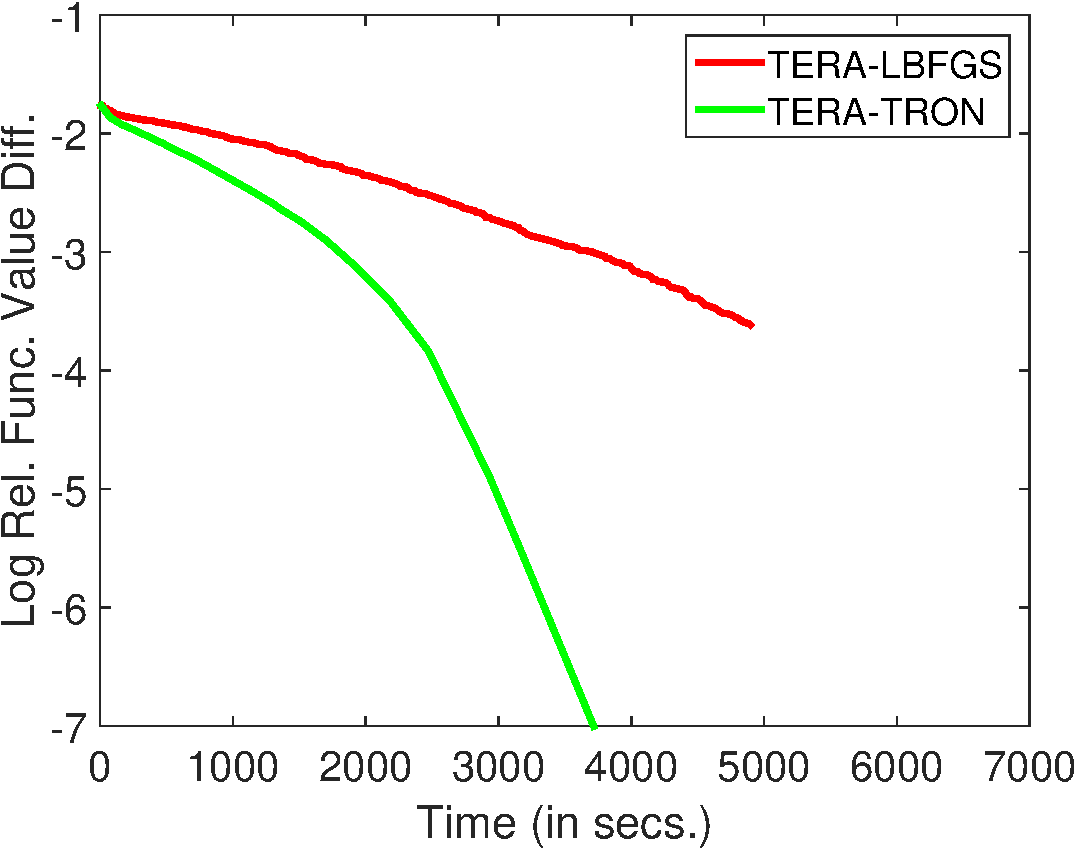
\includegraphics[width=0.46\linewidth]{tronlbfgsplots/kdd_8-crop}
}
\subfigure[{\it{kdd2010}} - 128 nodes]{
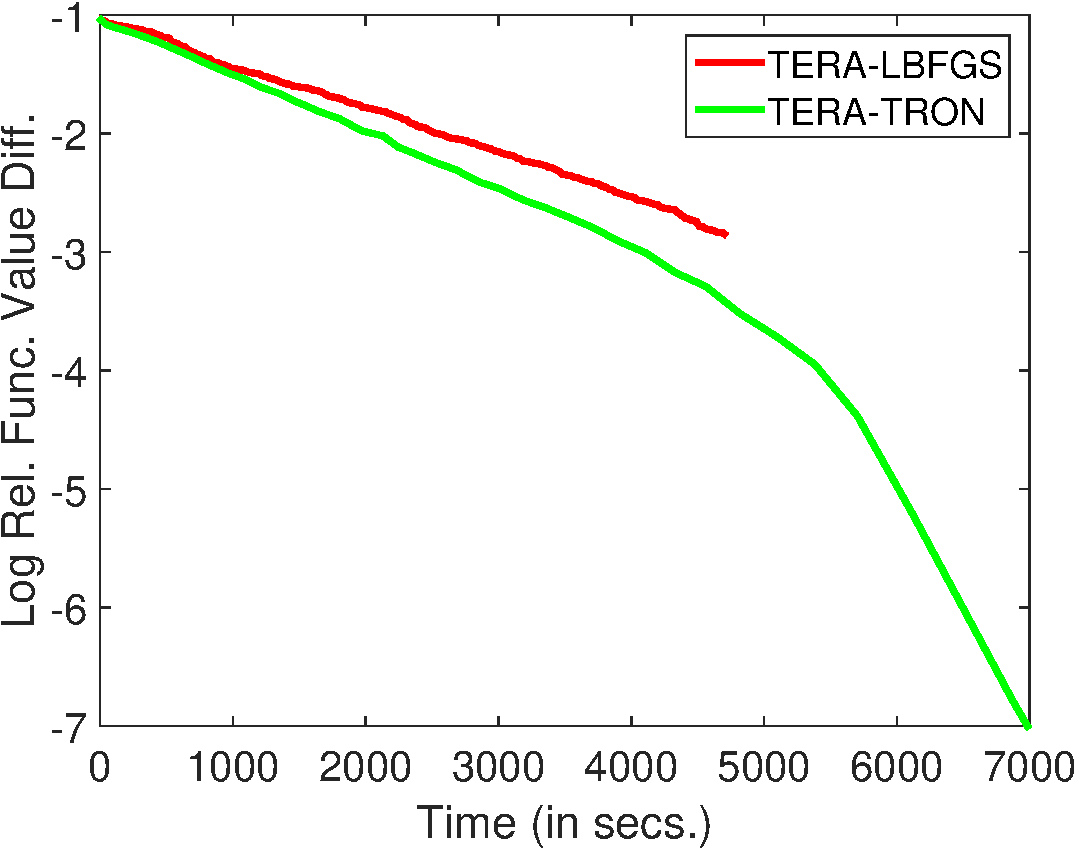
\includegraphics[width=0.46\linewidth]{tronlbfgsplots/kdd_128-crop}
}
\caption{Plots showing the time efficiency of TERA methods for {\it kdd2010}.}
\label{fig:tera}
\end{figure}

%\Kee{Is this ADMM subsection really needed? Discuss with Dhruv.}

\subsection{Study of ADMM}
\label{subsec:admm}

The ADMM objective function~\citep{Boyd2011} has a quadratic proximal term called augmented Lagrangian with a penalty parameter $\rho$ multiplying it. In general, the performance of ADMM is very sensitive to the value of $\rho$ and hence making a good choice for it is crucial. We consider three methods for choosing $\rho$.

Even though there is no supporting theory, Boyd et al~\citep{Boyd2011} suggest an approach by which $\rho$ is adapted in each iteration; see Equation (3.13) in Section 3.4.1 of that paper. We will refer to this choice as {\it Adap}.

Recently, \citet{deng2012} proved a linear rate of convergence for ADMM under assumptions A1 and A2 (see Section~\ref{general}) on ADMM functions. As a result, their analysis also hold for the objective function in~(\ref{risk}). They also give an analytical formula to set $\rho$ in order to get the best theoretical linear rate constant. We will refer to this choice of $\rho$ as {\it Analytic}.

We also consider a third choice, {\it{ADMM-Search}} in which, we start with the value of $\rho$ given by {\it Analytic}, choose several values of $\rho$ in its neighborhood and select the best $\rho$ by running ADMM for 10 iterations and looking at the objective function value.  Note that this step takes additional time and causes a late start of ADMM.

Figure~\ref{fig:admm} compares the progress of the training objective function for the three choices on {\it kdd2010} for $P=8$ and $P=128$.
{\it Analytic} is an order of magnitude slower than the other two choices. {\it Search} works well. However, a significant amount of initial time is spent on finding a good value for $\rho$, thus making the overall approach slow. {\it Adap} comes out to be the best performer among the three choices. Similar observations hold for other datasets and other choices of $P$. So, for ADMM, we will fix {\it Adap} as the way of choosing $\rho$ and refer to ADMM-{\it Adap} simply as ADMM.

It is also worth commenting on methods related to ADMM. Apart from ADMM,~\citet{bertsekas1997} discuss several other classic optimization methods for separable convex programming, based on proximal and Augmented Lagrangian ideas which can be used for distributed training of linear classifiers. ADMM represents the best of these methods. Also, Gauss-Seidel and Jacobi methods given in~\citet{bertsekas1997} are related to feature partitioning, which is very different from the example partitioning scenario studied in this paper. Therefore we do not consider these methods.

\begin{figure}[t]
\centering
\subfigure[{\it{kdd2010}} - 8 nodes]{
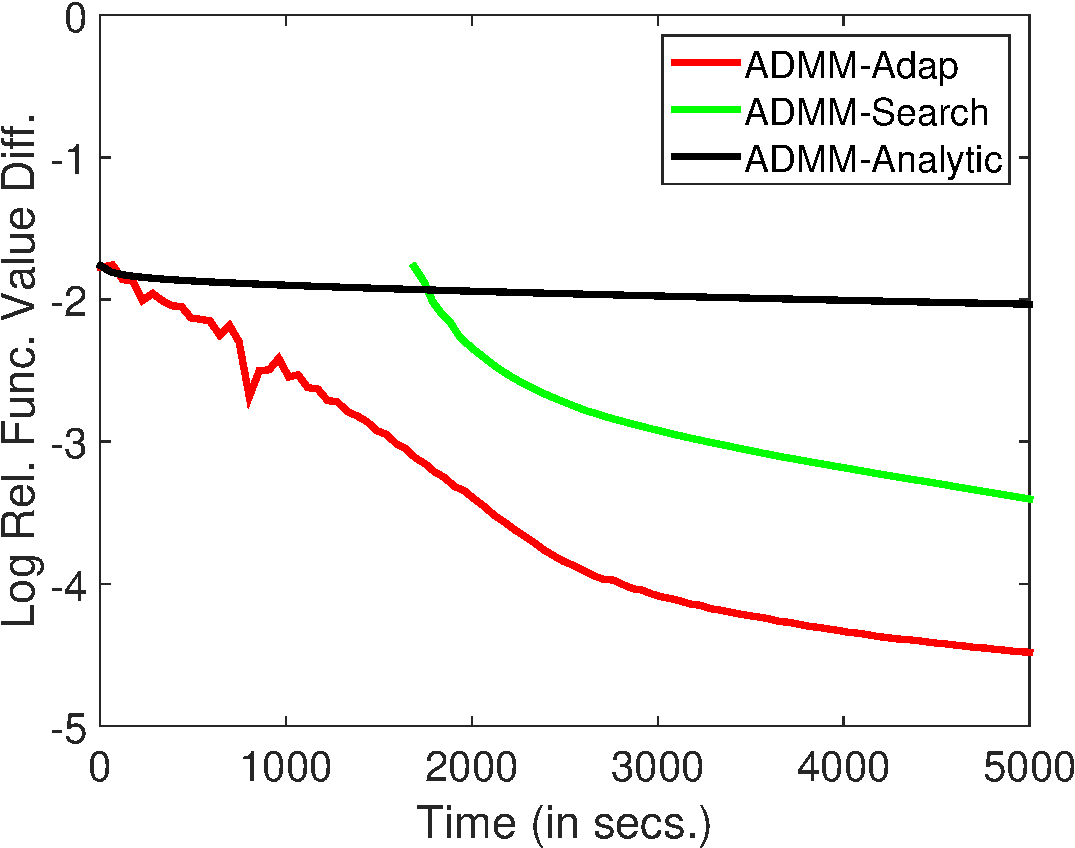
\includegraphics[width=0.46\linewidth]{admm/kdd_8-crop}
}
\subfigure[{\it{kdd2010}} - 128 nodes]{
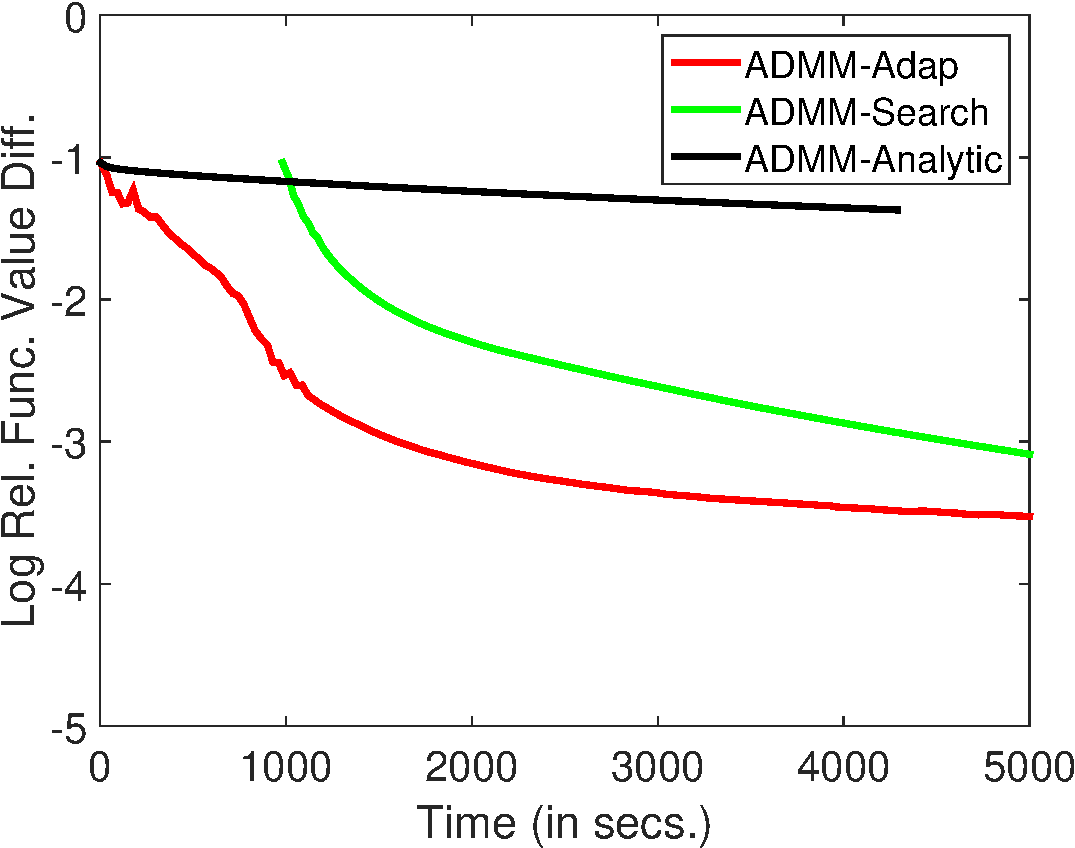
\includegraphics[width=0.46\linewidth]{admm/kdd_128-crop}
}
\caption{Plots showing the time efficiency of ADMM methods for {\it kdd2010}.}
\label{fig:admm}
\end{figure}



\subsection{Study of CoCoA}
\label{subsec:dbca}

In CoCoA~\citep{jaggi2014} the key parameter is the approximation level of the inner iterations used to solve each projected dual sub-problem. The number of epochs of coordinate dual ascent inner iterations plays a crucial role. We try the following choices for it: 0.1, 1 and 10.\footnote{The examples were randomly shuffled for presentation. When the number of epochs is a fraction, e.g., 0.1, the inner iteration was stopped after 10\% of the examples were presented.} Figure~\ref{fig:cocoa} compares the progress of the objective function on {\it kdd2010} for two choices of nodes, $P=8$ and $P=128$. We find the choice of 1 epoch to work well reasonably consistently over all the five datasets and varying number of nodes. So we fix this choice and refer to the resulting method simply as CoCoA. Note in Figure~\ref{fig:cocoa} that the (primal) objective function does not decrease continuously with time. This is because it is a dual method and so monotone descent of the objective function is not assured.\footnote{The same comment holds for ADMM which is also a dual method; see for example, the jumps in objective function values for ADMM in Figures~\ref{fig:commpass1} and \ref{fig:timepass1} for {\it kdd2010}.}

\begin{figure}[t]
\centering
\subfigure[{\it{kdd2010}} - 8 nodes]{
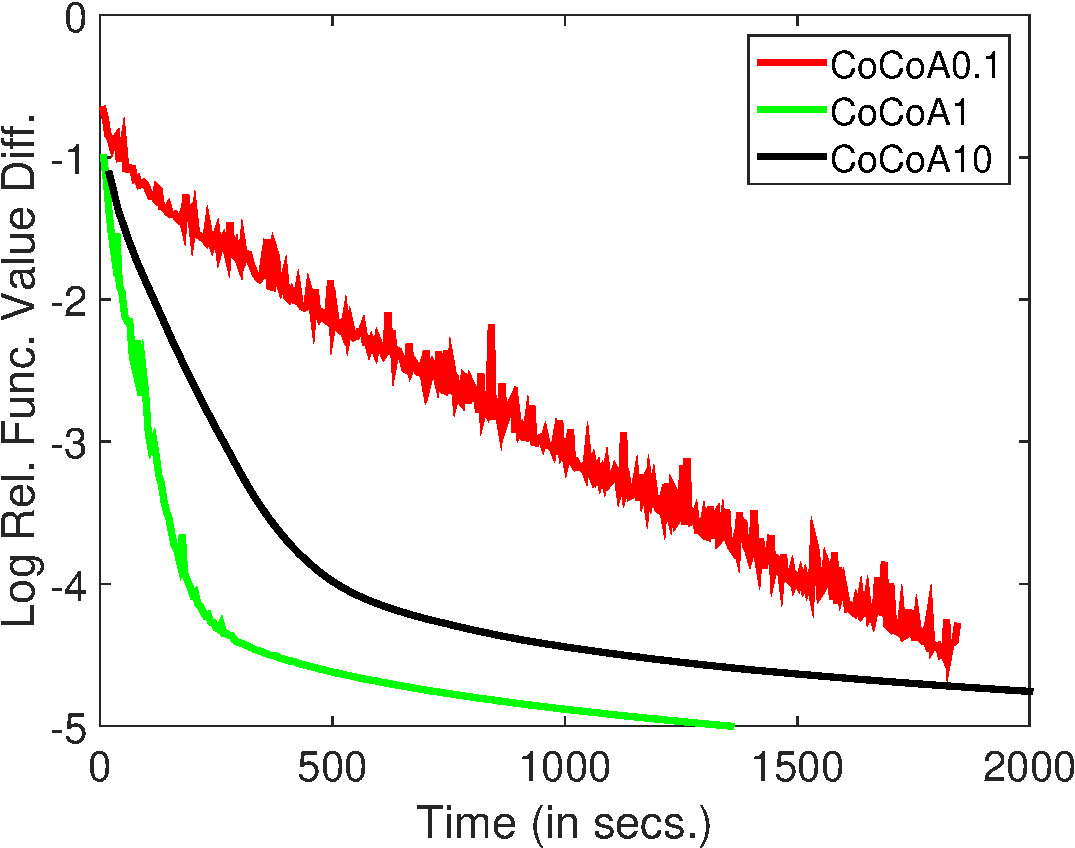
\includegraphics[width=0.46\linewidth]{pbdplots/kdd_8-crop}
}
\subfigure[{\it{kdd2010}} - 128 nodes]{
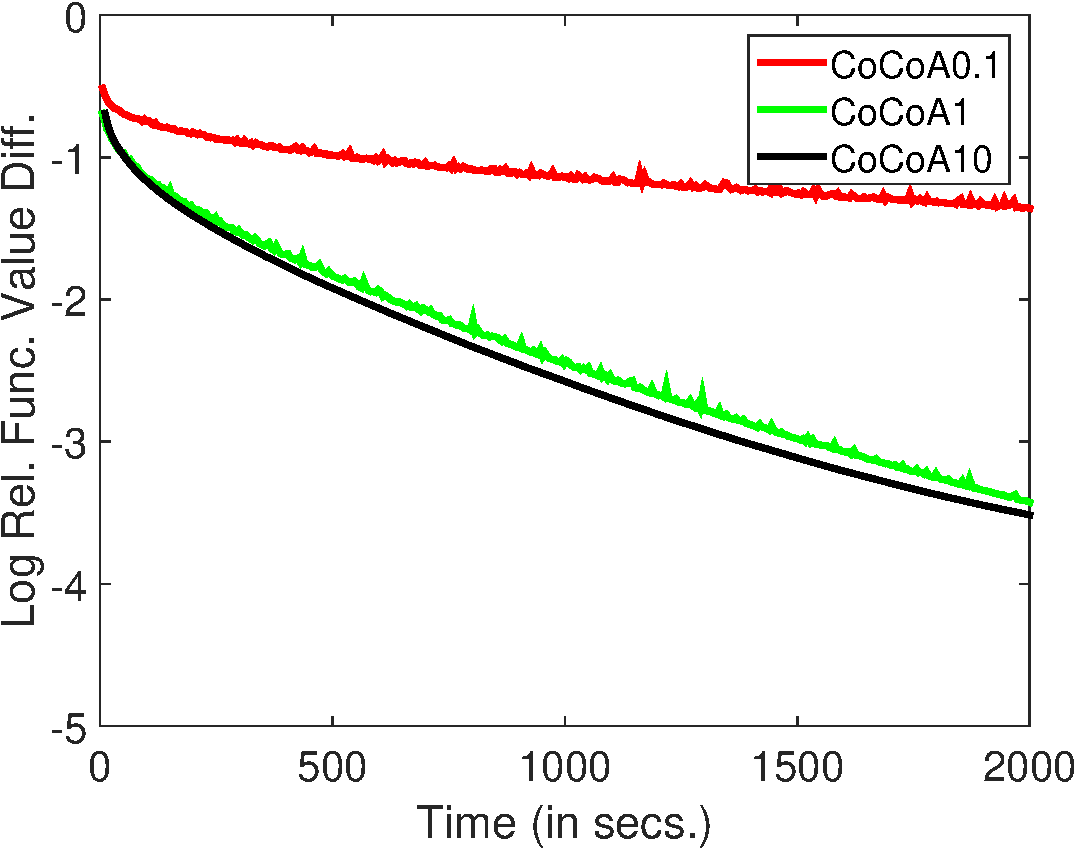
\includegraphics[width=0.46\linewidth]{pbdplots/kdd_128-crop}
}
\caption{Plots showing the time efficiency of CoCoA settings for {\it kdd2010}.}
\label{fig:cocoa}
\end{figure}

%\Kee{The subsection below has been newly added.}

\subsection{Study of DANE}
\label{subsec:dane}

In our detailed comparison study later in this section, we will also include another method called DANE, which has some resemblance to FADL. This is the Newton based method described in~\citet{sharir2014}. Even though this method is very different in spirit from our method, it uses a function approximation similar to our Nonlinear approximation idea; we briefly discussed this in Subsection~\ref{subsec:fhatp}. DANE is a non-monotone method that is based on fixed step sizes, with a probabilistic convergence theory to support it.

DANE has two parameters, $\mu$ and $\eta$ in the function approximation; $\mu$ is the coefficient for the proximal term and $\eta$ is used for defining the direction. \citet{sharir2014} do not prove convergence for any possible choices of $\mu$ and $\eta$ values; their practical recommendation is to use $\mu=3\lambda$ and $\eta=1$. The choice of $\mu$ in particular, turns out to be quite sub-optimal. We found that there was no single value of $\mu$ that is good for all datasets, and so it needs to be tuned for each dataset. So, to improve DANE, we included an initial $\mu$-tuning step. We start with $\mu=3*\lambda$ and use an initial set of four outer iterations to choose the $\mu$ value that gives the best improvement in objective function. Starting from $\mu=3*\lambda$ we try several values of $\mu$ in the direction of $\mu$ change that leads to improvement. After the first four outer iterations, we fix $\mu$ at the chosen best value for the remaining iterations. (Note that the cost associated with tuning $\mu$ has to be included in the overall cost of DANE.) As we will see later in Subsection~\ref{subsec:overallcomp}, in spite of all this tuning, DANE did not converge in several situations. Essentially, the issue is that $\mu$ has to be adaptive - DANE needs to use different choices of $\mu$ in the early, middle and end stages of one training. But then, this is nearly akin to doing a kind of line search in each outer iteration. As opposed to DANE, note that FADL is a monotone method directly based on line search, and it does not need the proximal term to restrict step-sizes. Also, unlike DANE, all the parameters of FADL are fixed to default values for all datasets.

The choice of inner optimizer for DANE is crucial for its efficiency. We tried SVRG~\citep{johnson2013} and also TRON~\citep{lin2008}. Both did well, but SVRG was better, especially for small number of nodes. So we did a more detailed study of SVRG. We tried two choices. (a) Fix the number of epochs for the local (inner) optimization to some good value, e.g., 10. (b) Always choose the number of epochs for the local (inner) optimization to be such that the cost of local computation in a node is matched with the communications cost. Choice (b) gave a better solution. So we have used it for DANE.



%\Kee{Changes have been made below.}

\subsection{Study of FADL}
\label{subsec:our}

Recall from Subsection~\ref{subsec:fhatp} the various choices that we suggested for $\fhat_p$.
We are yet to implement and study the BFGS approximation; we leave it out for future work.
Our original work~\citep{dhruv2013} focused on the Linear approximation, but we found the Quadratic, Hybrid and Nonlinear choices to work much better. So we study only these three methods. The implementation of these methods is as described in Subsection~\ref{subsec:practical} and Algorithm~\ref{alg:fadl}.

Figure~\ref{fig:ipm} compares the progress of the training objective function for various choices of $\fhat_p$. Among the choices, the quadratic approximation for $\fhat_p$ gives the best performance, although the Hybrid and Nonlinear approximations also do quite well. We observe this reasonably consistently in other datasets too. Hence, from the set of methods considered in this subsection we choose FADL-Quadratic approximation as the only method for further analysis, and simply refer to this method as FADL hereafter.

Why does the quadratic approximation do better than hybrid and nonlinear approximations? We do not have a precise answer to this question, but we give some arguments in support.
In each outer iteration, the function approximation idea is mainly used to get a good direction. Recall from Subsection~\ref{subsec:fhatp} that different choices use different approximations for $\Ltilde_p$ and $\Lhat_p$. Using the same ``type" (meaning linear, nonlinear or quadratic) for both, $\Ltilde_p$ and $\Lhat_p$ is possibly better for direction finding. Second, the direction finding could be more sensitive to the nonlinear approximation compared to the quadratic approximation; this could become more severe as the number of nodes becomes larger. Literature shows that quadratic approximations have good robustness properties; for example, subsampling in Hessian computation~\citep{byrd2012} doesn't worsen direction finding much.

\begin{figure}[t]
\centering
\subfigure[{\it{kdd2010}} - 8 nodes]{
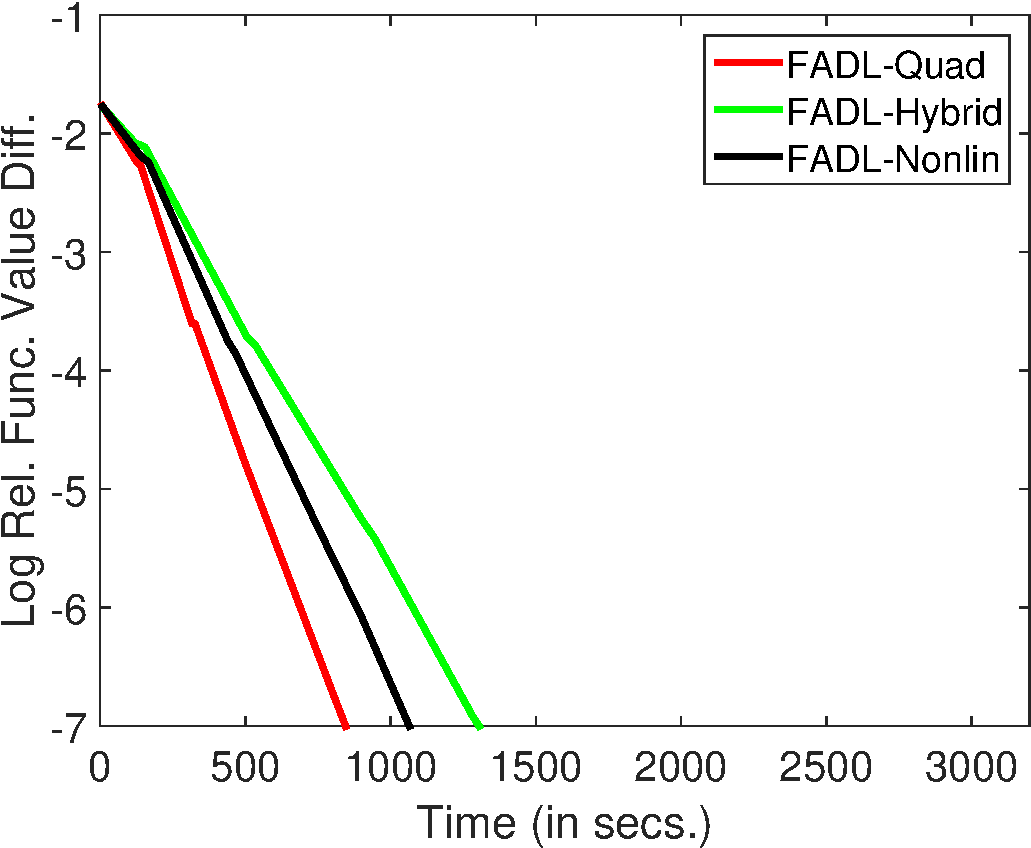
\includegraphics[width=0.46\linewidth]{ipmplots/kdd_8-crop}
}
\subfigure[{\it{kdd2010}} - 128 nodes]{
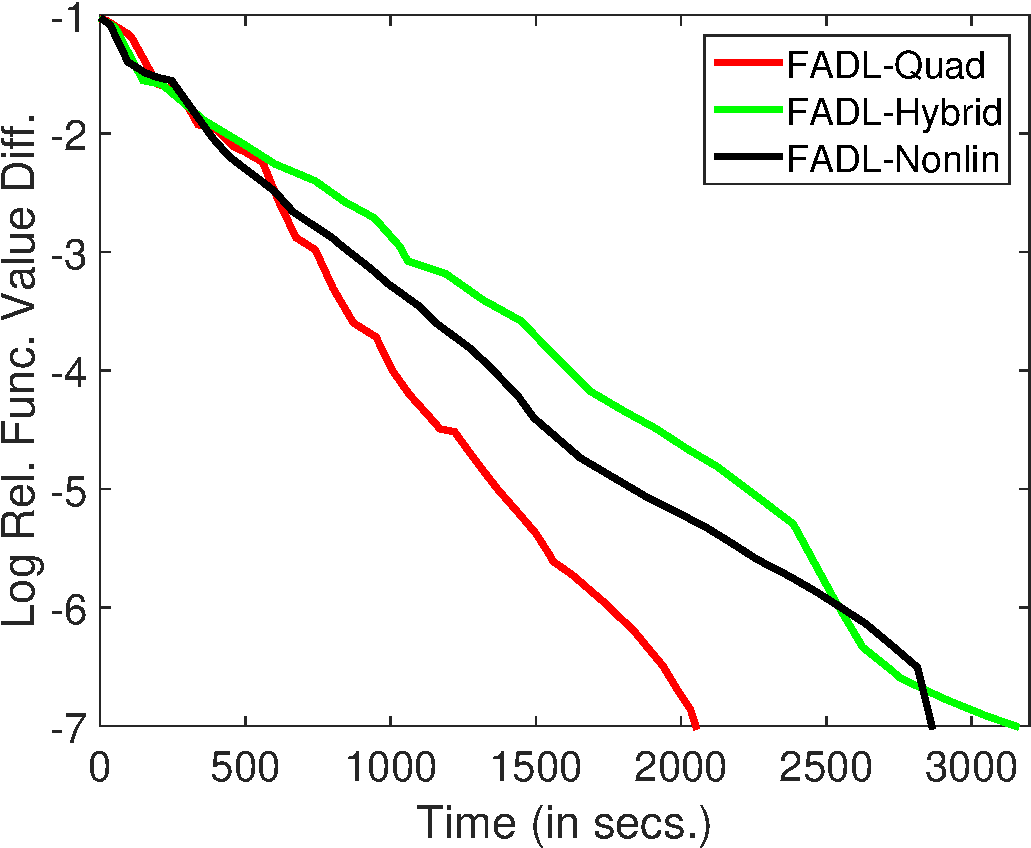
\includegraphics[width=0.46\linewidth]{ipmplots/kdd_128-crop}
}

\caption{Plots showing the time efficiency of the three function approximations of FADL for {\it kdd2010}.}
\label{fig:ipm}
\end{figure}

%\Kee{The subsection below is newly added.}

\subsection{Comparison of FADL against DiSCO}
\label{subsec:discocomp}

DiSCO~\citep{discoicml} is an inexact damped Newton method, where the inexact Newton steps are computed using a distributed preconditioned conjugate gradient method. Like TERA, it belongs to the SQM class~\citep{chu2006}. The DiSCO method as described in~\citet{discoicml} is not designed for squared hinge loss. Therefore, in this subsection we separately compare FADL against DiSCO using the logistic loss. With communication efficiency in mind we compare the two methods in terms of the number of communication passes. Figure~\ref{fig:commpassD1} gives the progress in objective function as a function of the number of communication passes for the two methods. FADL is clearly better than DiSCO, the difference being quite large on datasets such as {\it kdd2010}. In terms of total computing time, the superiority of FADL turns out to be even better than what is seen in the plots of communication passes. This is because DiSCO requires more extensive computational steps than FADL within one communication pass.

\subsection{Comparison of FADL against TERA, ADMM, CoCoA and DANE}
\label{subsec:overallcomp}

Having made the best choice of settings for the methods, we now evaluate FADL against TERA, ADMM, CoCoA and DANE in more detail. We do this using three sets of plots. We give details only for $P=8$ and $P=128$ to give an idea of how performance varies for small and large number of nodes.
\begin{enumerate}
\item {\it Communication passes.} We plot the variation of the training objective function as a function of the number of communication passes. For the $x$-axis we prefer the number of communication passes instead of the number of outer iterations since the latter has a different meaning for different methods while the former is quite uniform for all methods. Figures~\ref{fig:commpass1} and~\ref{fig:commpass2} give the plots respectively for the large dimensional ($m$ large) datasets ({\it kdd2010}, {\it url} and {\it webspam}) and medium/small dimensional ($m$ medium/small) datasets ({\it mnist8m} and {\it rcv}).
\item {\it Time.} We plot the variation of the training objective function as a function of the actual solution time. Figures~\ref{fig:timepass1} and~\ref{fig:timepass2} give the plots respectively for the large dimensional and medium/small dimensional datasets.
\item {\it Speed-up over TERA.} TERA is an established strong baseline method. So it is useful to ask how other methods fare relative to TERA and study this as a function of the number of nodes. For doing this we need to represent each method by one or two real numbers that indicate performance. Since generalization performance is finally the quantity of interest, we stop a method when it reaches within 0.1\% of the steady state AUPRC value achieved by full, perfect training of~(\ref{risk}) and record the following two measures: the total number of communication passes and the total time taken. For each measure, we plot the ratio of the measure's value for TERA to the corresponding measure's value for a method, as a function of the number of nodes, and repeat this for each method. Larger this ratio, better is a method; also, ratio greater than one means a method is faster than TERA. Figures~\ref{fig:auprcpass} and~\ref{fig:auprctime} give the plots for all the five datasets.
\end{enumerate}
Let us now use these plots to compare the methods. In the plots, DANE starts later than other methods due to the extra work needed for tuning the proximal parameter $\mu$.

\subsubsection{Rate of Convergence}
\label{subsubsec:rate}

Analysis of the rate of convergence is better done by studying the behavior of the training objective function with respect to the number of communication passes. So it is useful to look at Figures~\ref{fig:commpass1} and~\ref{fig:commpass2}. Clearly, as predicted by theory, the rate of convergence is linear for all methods.

%\Kee{Try to move Figure 5 up here.}

\begin{figure}[H]
\centering
\subfigure[{\it{kdd2010}} - 8 nodes]{
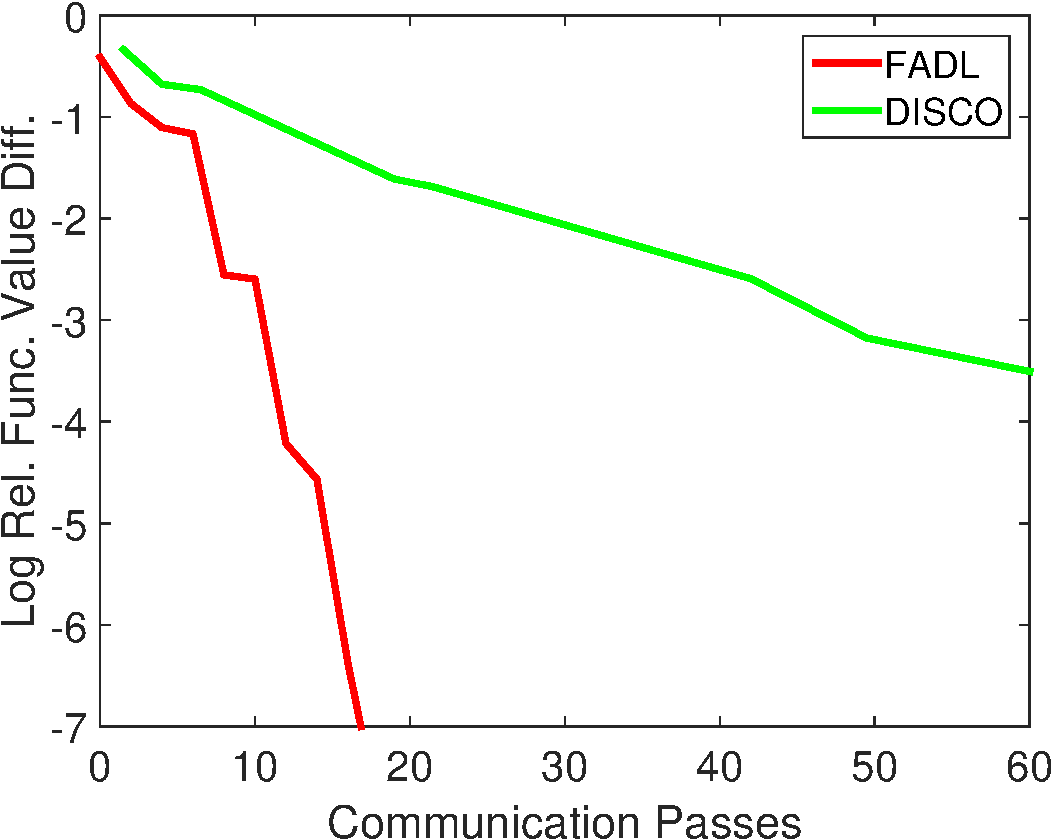
\includegraphics[width=0.46\linewidth]{discoplots/kdd_8-crop}
}
\subfigure[{\it{kdd2010}} - 128 nodes]{
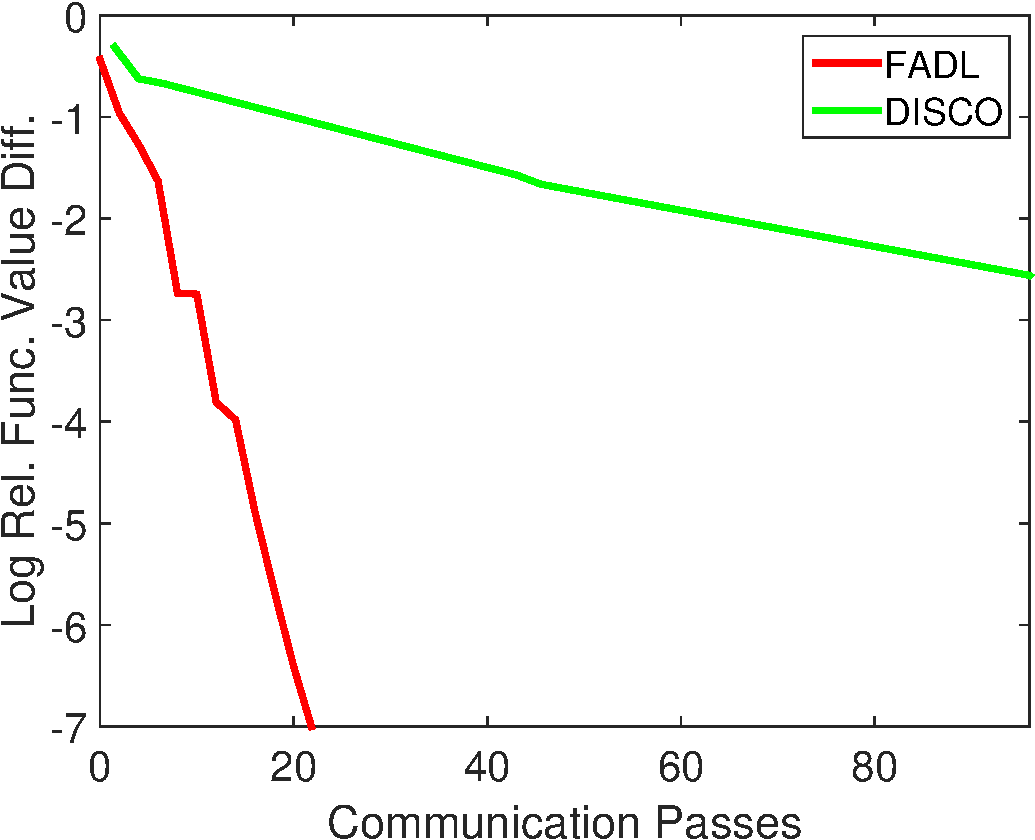
\includegraphics[width=0.46\linewidth]{discoplots/kdd_128-crop}
}

\subfigure[{\it{url}} - 8 nodes]{
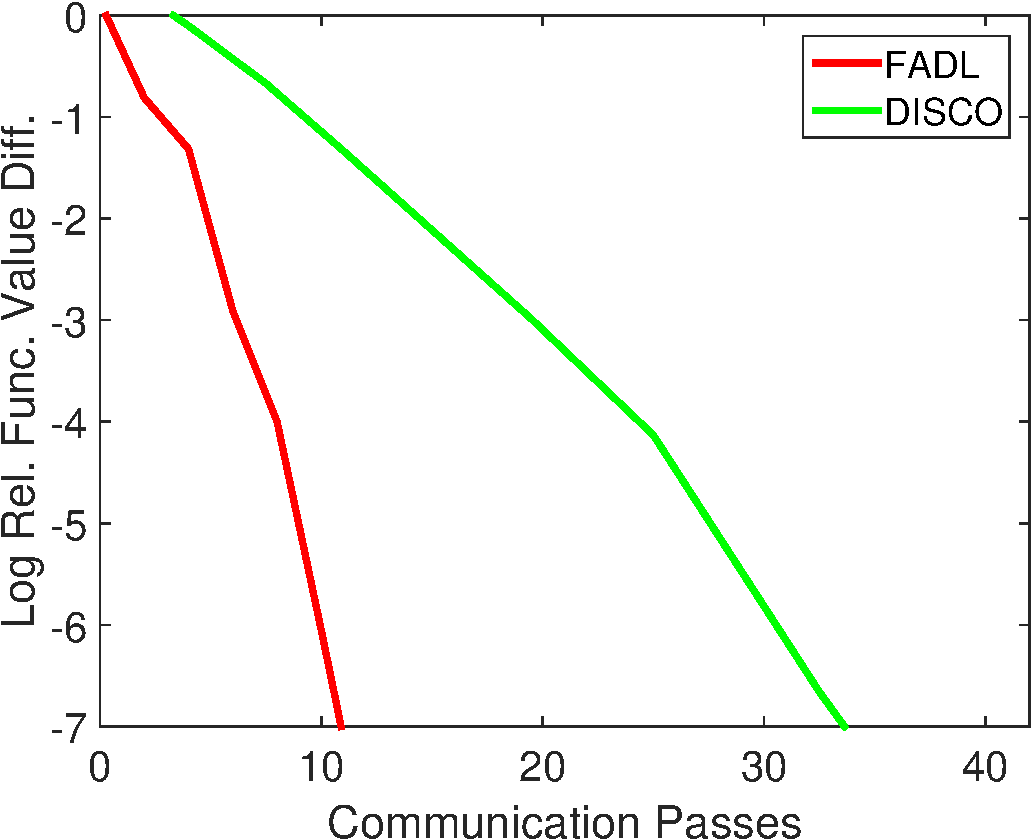
\includegraphics[width=0.46\linewidth]{discoplots/url_8-crop}
}
\subfigure[{\it{url}} - 128 nodes]{
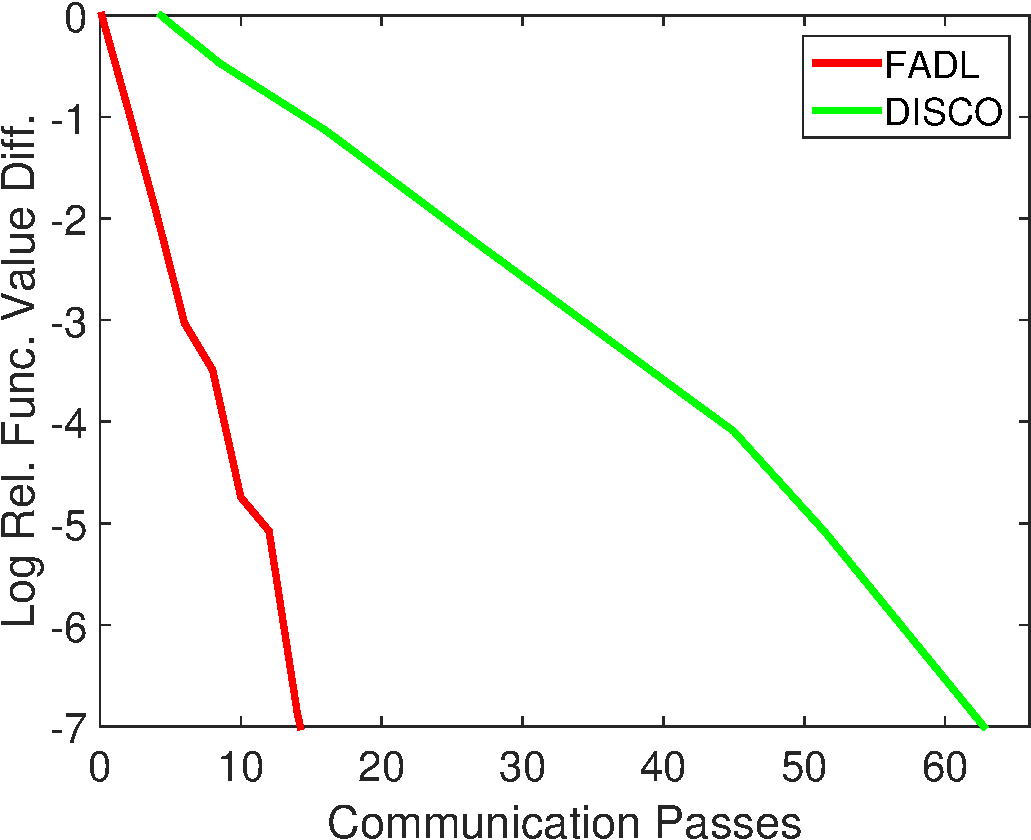
\includegraphics[width=0.46\linewidth]{discoplots/url_128-crop}
}

\subfigure[{\it{webspam}} - 8 nodes]{
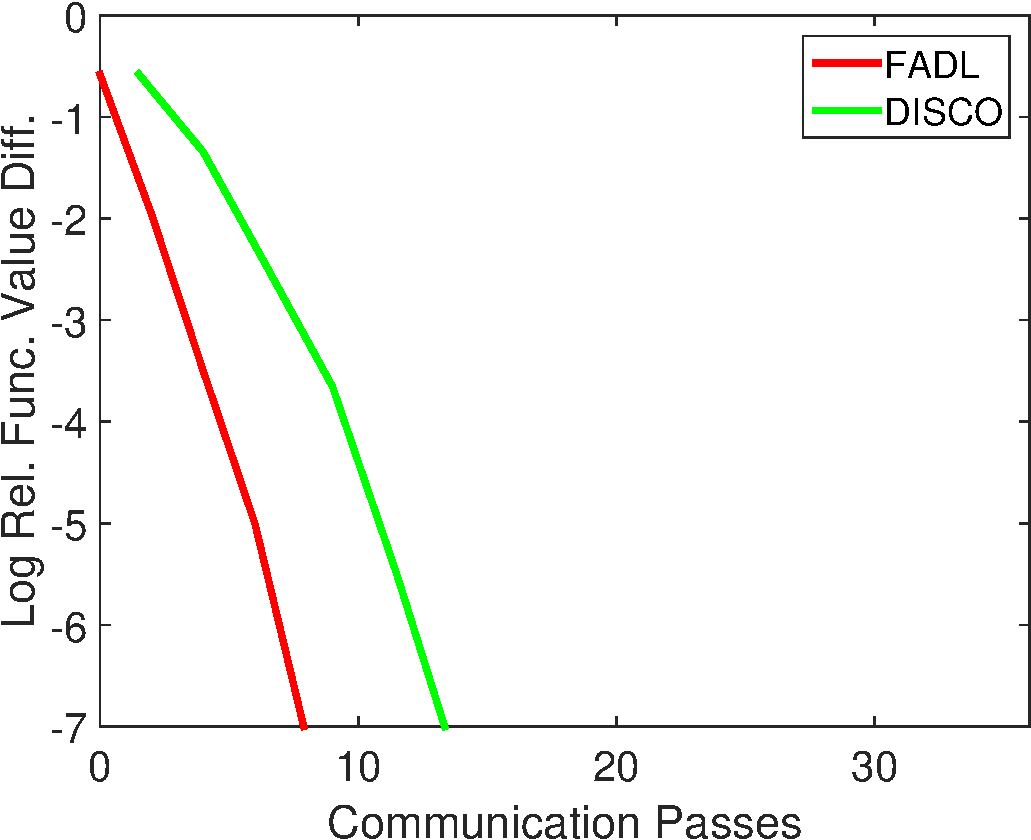
\includegraphics[width=0.46\linewidth]{discoplots/rcv_8-crop}
}
\subfigure[{\it{webspam}} - 128 nodes]{
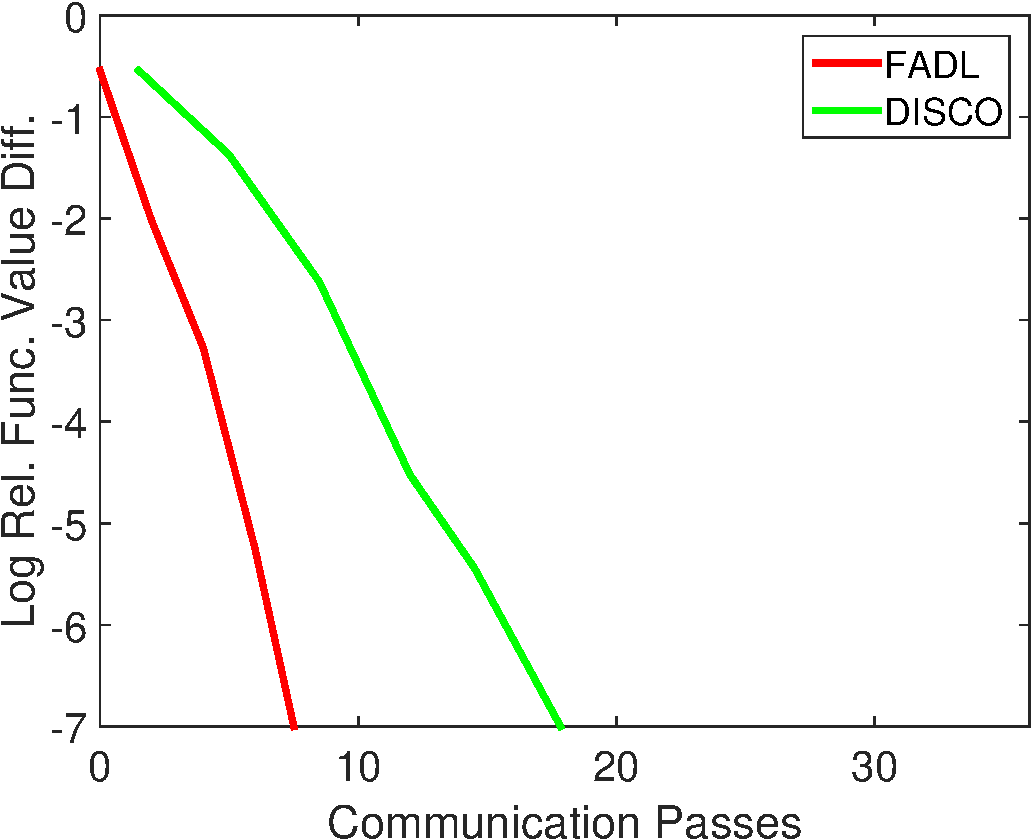
\includegraphics[width=0.46\linewidth]{discoplots/rcv_128-crop}
}

\caption{Plots comparing the number of communication passes of DiSCO and FADL on three datasets.}
\label{fig:commpassD1}
\end{figure}


\begin{figure}[H]
\centering
\subfigure[{\it{kdd2010}} - 8 nodes]{
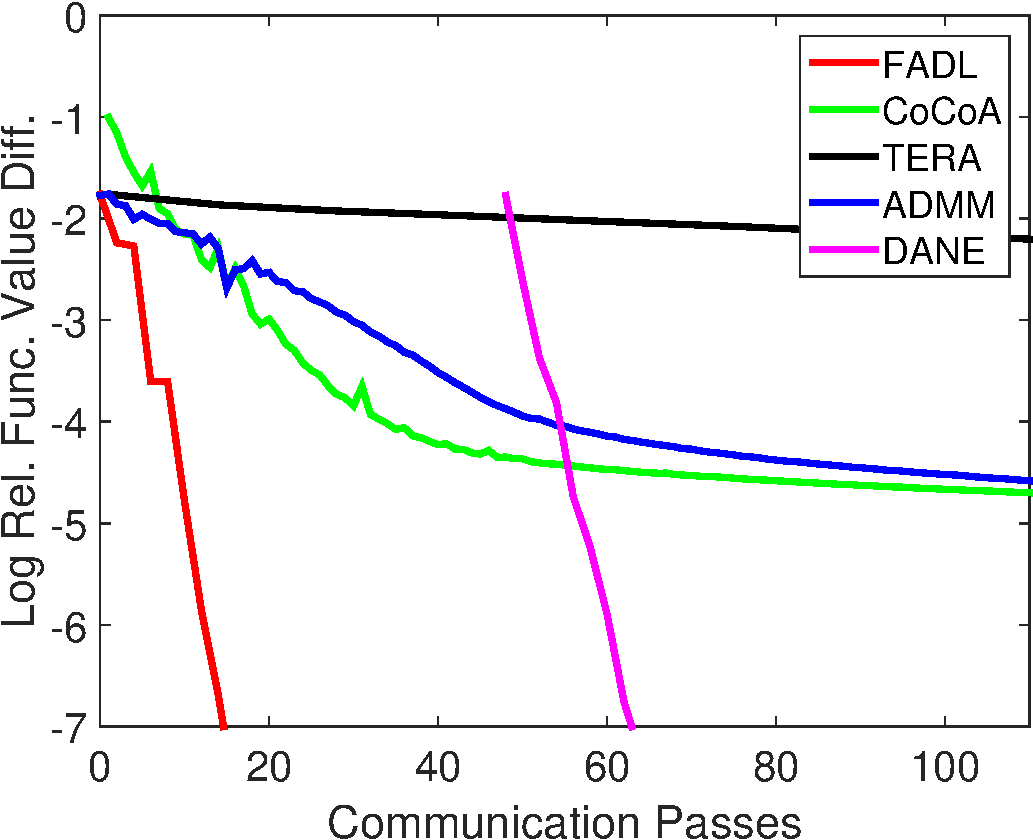
\includegraphics[width=0.46\linewidth]{overallobjvscommpassplots/kdd_8-crop}
}
\subfigure[{\it{kdd2010}} - 128 nodes]{
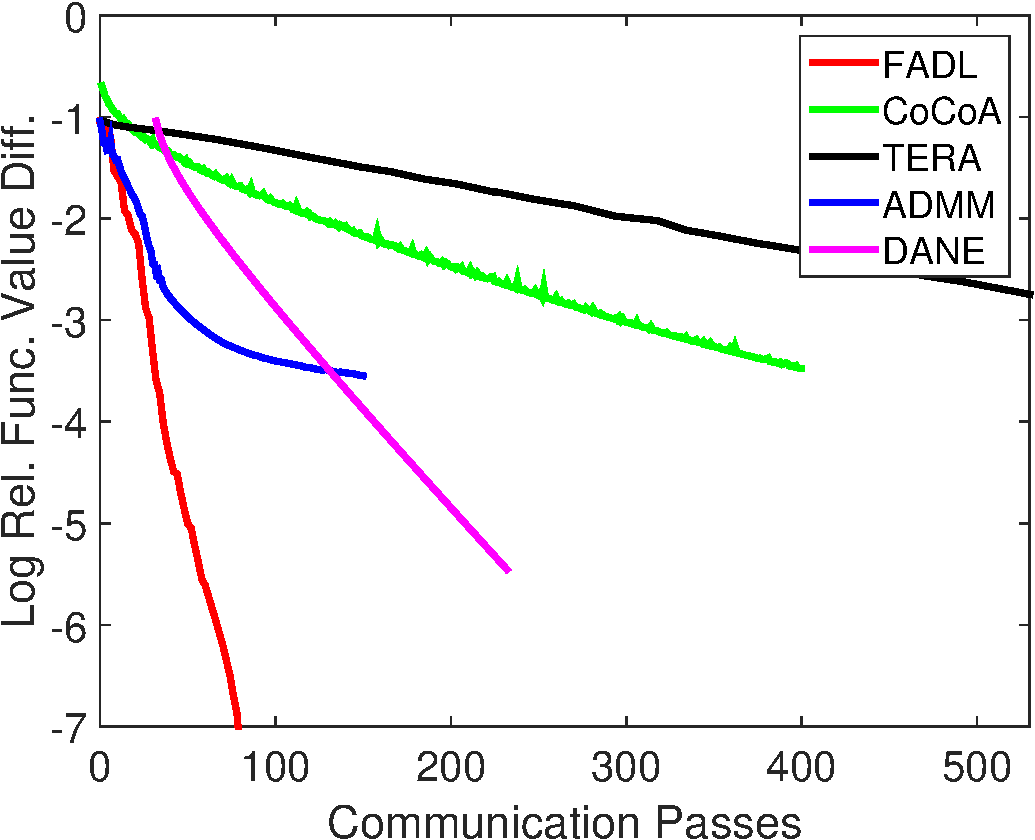
\includegraphics[width=0.46\linewidth]{overallobjvscommpassplots/kdd_128-crop}
}

\subfigure[{\it{url}} - 8 nodes]{
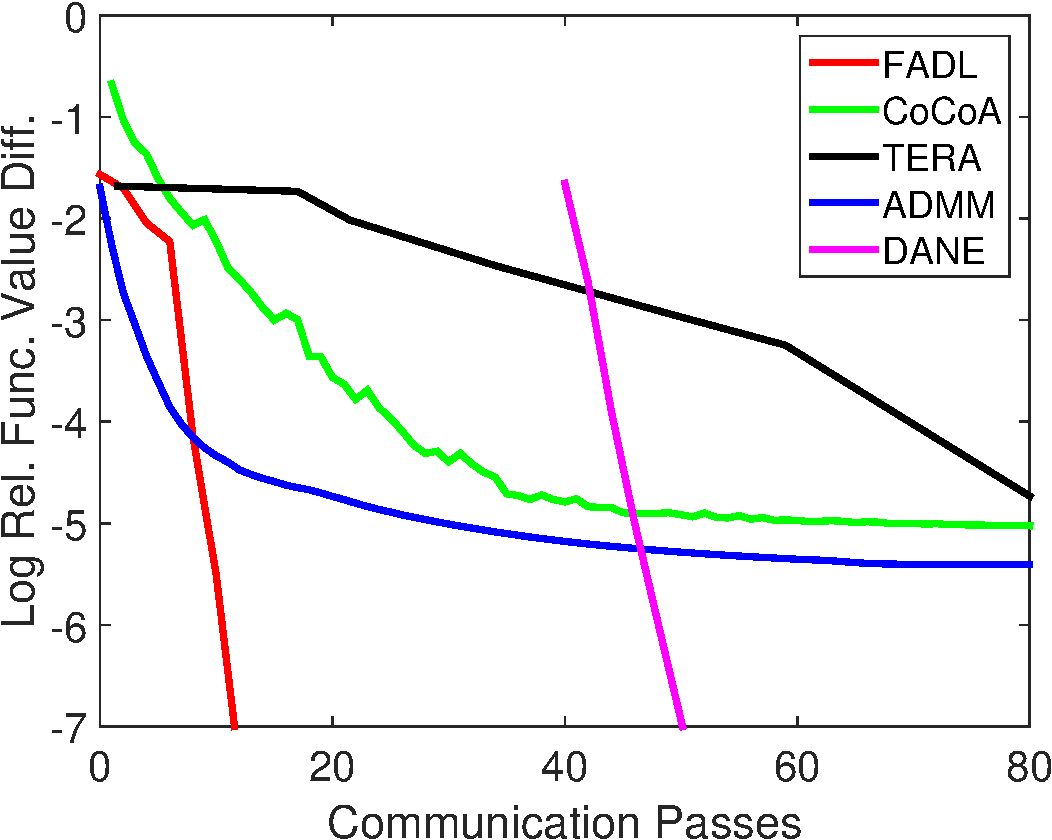
\includegraphics[width=0.46\linewidth]{overallobjvscommpassplots/url_8-crop}
}
\subfigure[{\it{url}} - 128 nodes]{
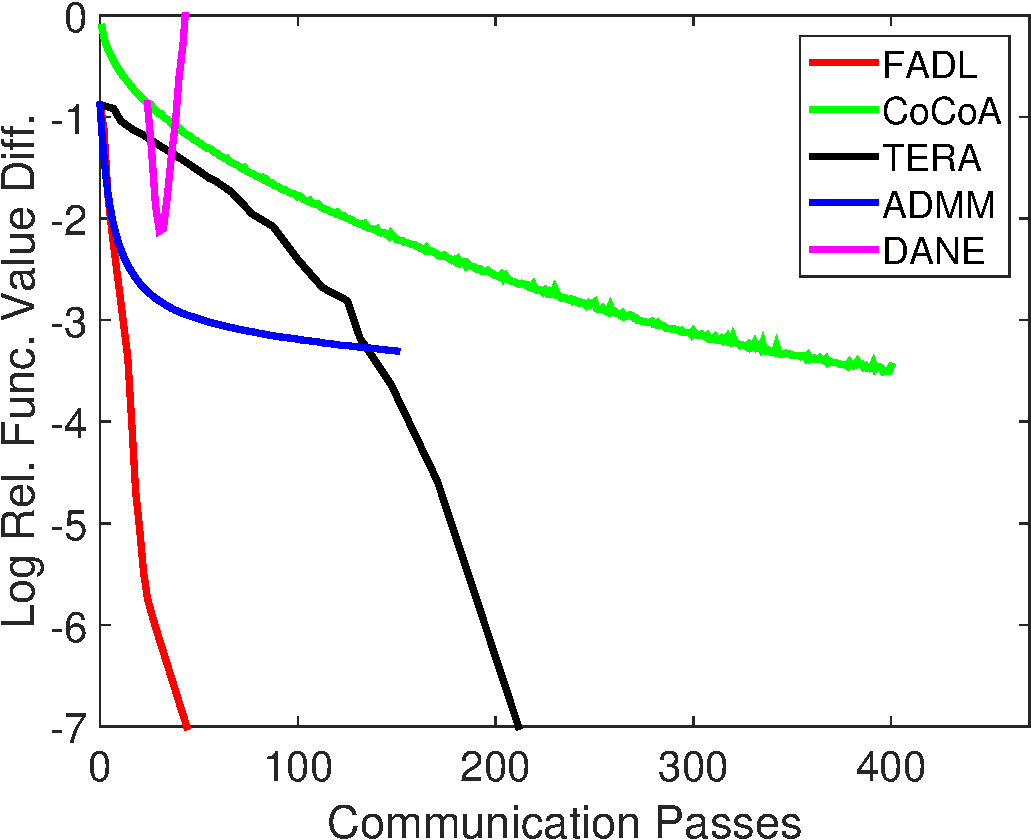
\includegraphics[width=0.46\linewidth]{overallobjvscommpassplots/url_128-crop}
}

\subfigure[{\it{webspam}} - 8 nodes]{
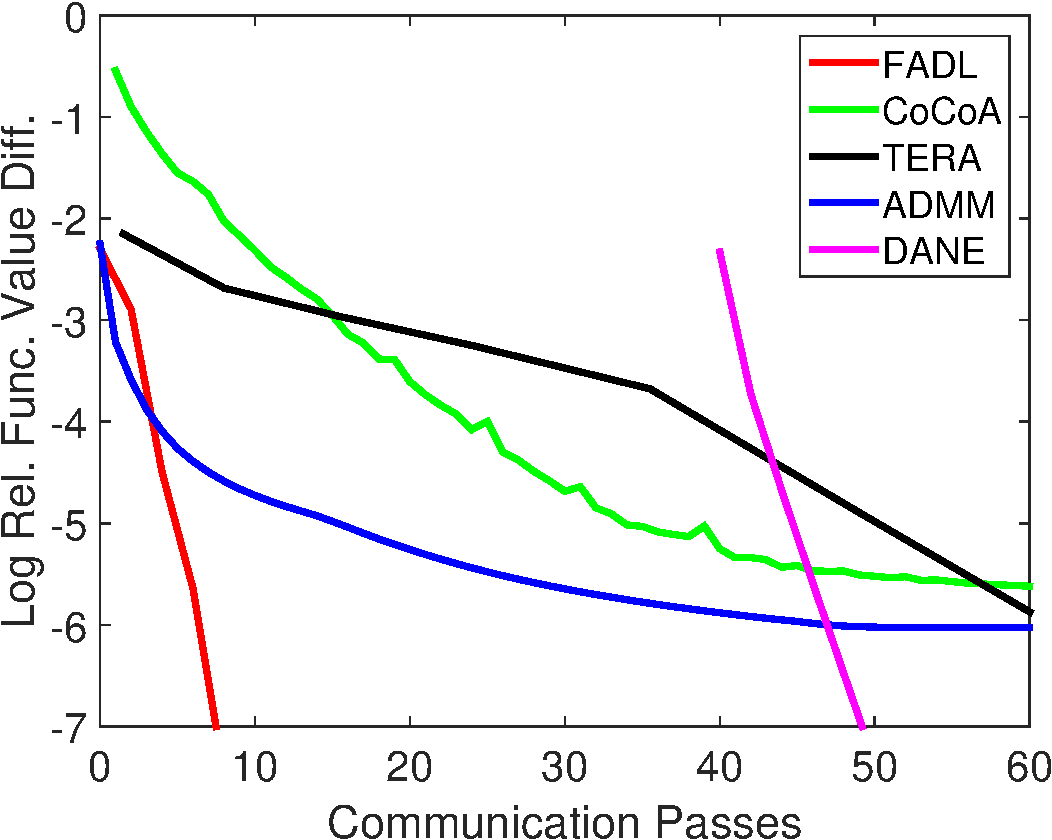
\includegraphics[width=0.46\linewidth]{overallobjvscommpassplots/webspam_8-crop}
}
\subfigure[{\it{webspam}} - 128 nodes]{
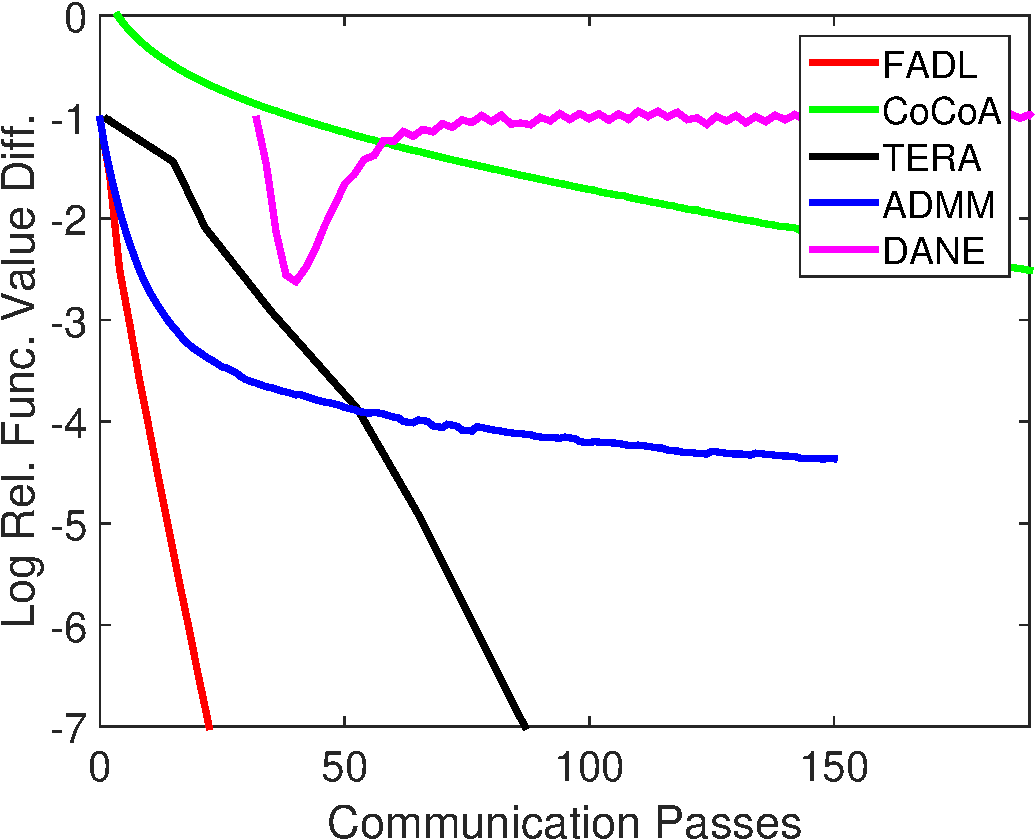
\includegraphics[width=0.46\linewidth]{overallobjvscommpassplots/webspam_128-crop}
}

\caption{Plots showing the rate of convergence of various methods for the three high dimensional datasets.}
\label{fig:commpass1}
\end{figure}

\begin{figure}[H]
\centering

\subfigure[{\it{mnist8m}} - 8 nodes]{
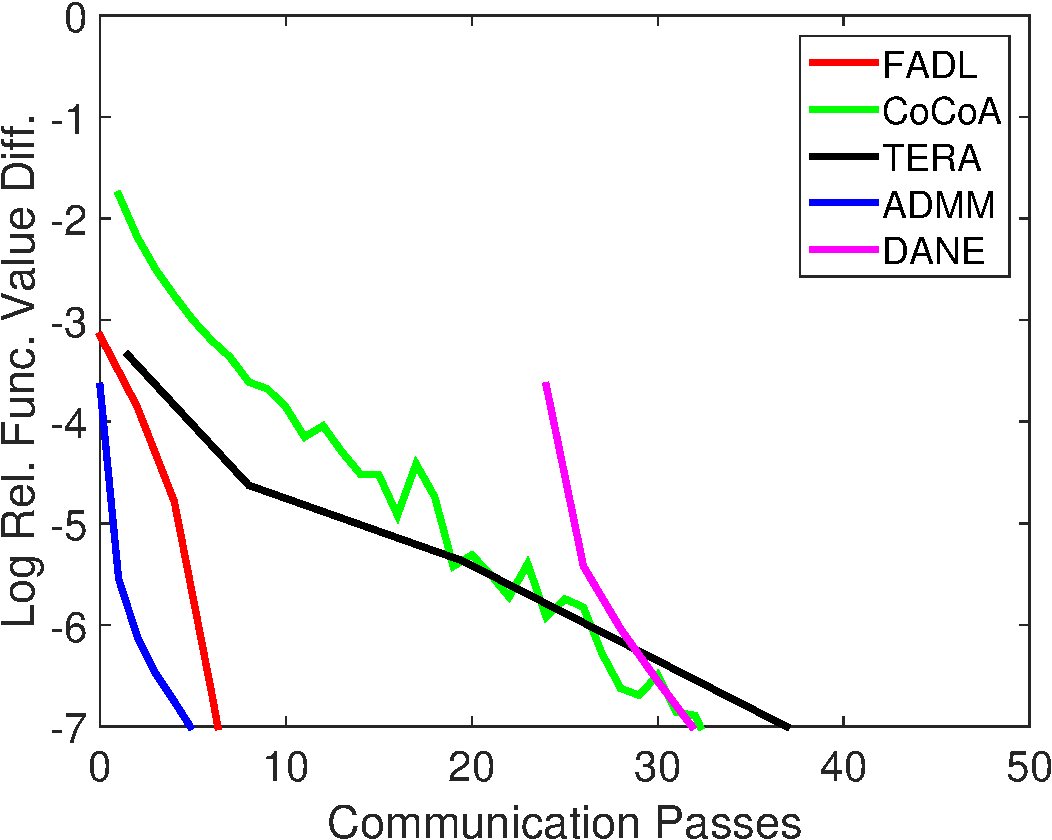
\includegraphics[width=0.46\linewidth]{overallobjvscommpassplots/mnist_8-crop}
}
\subfigure[{\it{mnist8m}} - 128 nodes]{
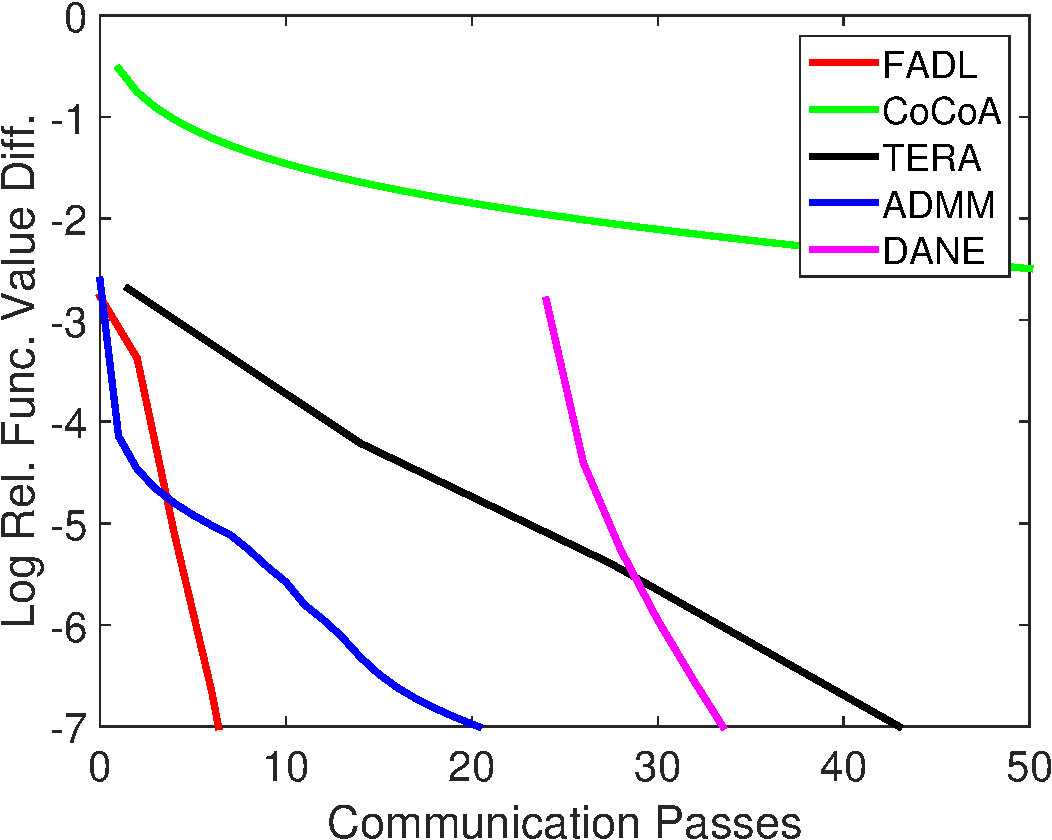
\includegraphics[width=0.46\linewidth]{overallobjvscommpassplots/mnist_128-crop}
}

\subfigure[{\it{rcv}} - 8 nodes]{
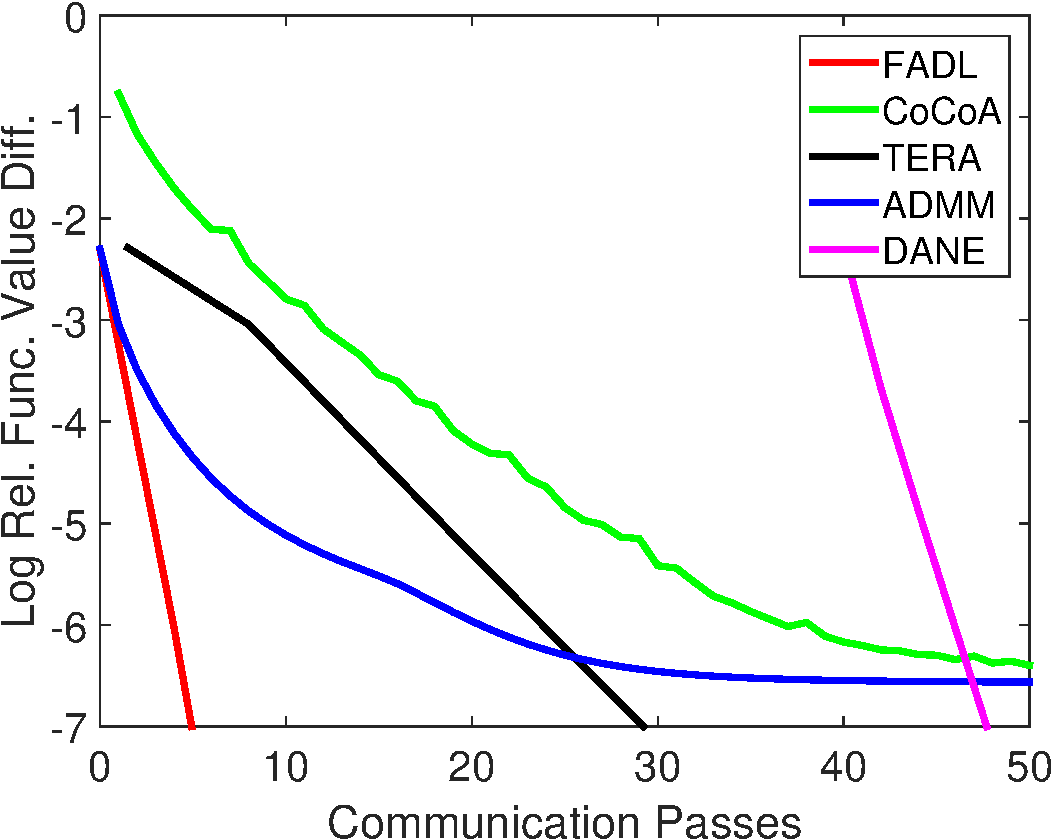
\includegraphics[width=0.46\linewidth]{overallobjvscommpassplots/rcv_8-crop}
}
\subfigure[{\it{rcv}} - 128 nodes]{
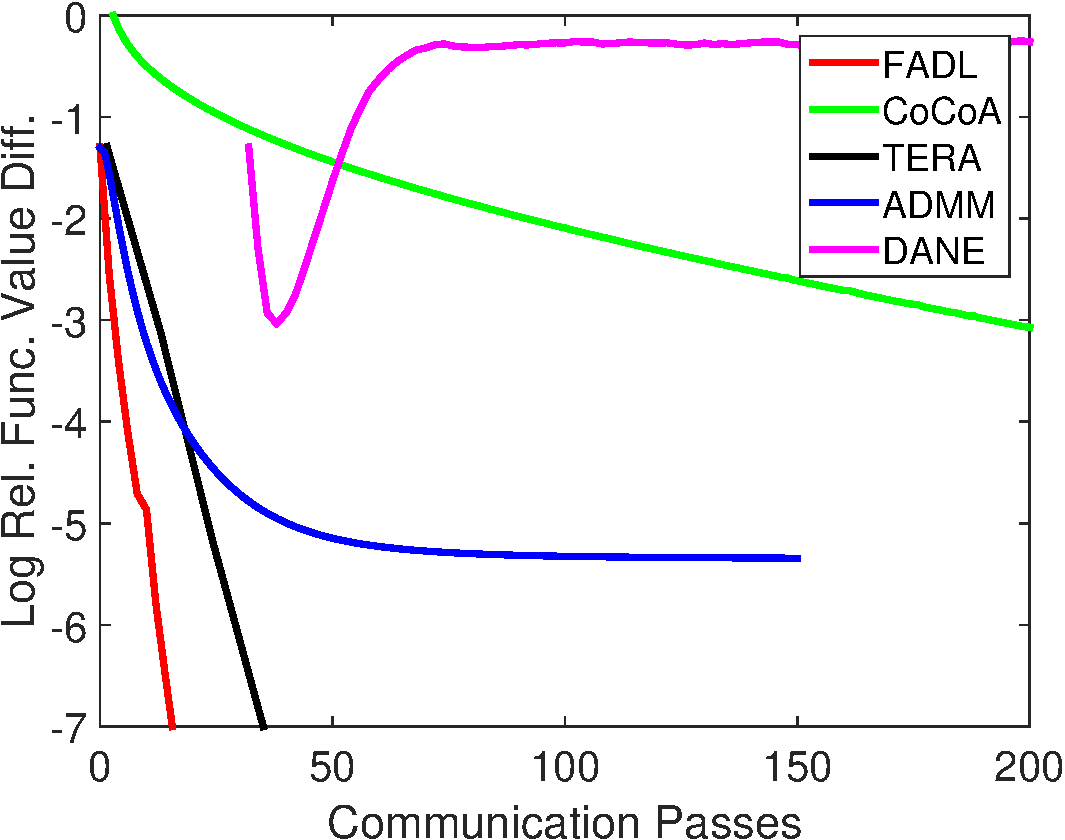
\includegraphics[width=0.46\linewidth]{overallobjvscommpassplots/rcv_128-crop}
}

\caption{Plots showing the linear convergence of various methods for the two low/medium dimensional datasets.}
\label{fig:commpass2}
\end{figure}


TERA uses distributed computation only to compute the gradient and so the plots should be unaffected by $P$. But in the plots we do see differences between the plots for $P=8$ and $P=128$. This is because of their different initialization (average of one pass SGD solutions from nodes): the initialization with lower number of nodes is better due its smaller variance; note also the better starting objective function value at the start (left most point) for $P=8$.

For FADL, the rate is steeper for $P=8$ than for $P=128$. This steeper behavior for lower number of nodes is expected because the functional approximation in each node becomes better as the number of nodes decreases.

Recall from Section~\ref{intro} that, our main aim behind the design of the function approximation based methods is to reduce the number of communication passes significantly. The plots in Figures~\ref{fig:commpass1} and~\ref{fig:commpass2} clearly confirm such a reduction.

Even though the end convergence rate of ADMM is slow, it generally shows good rates of convergence in the initial stages of training. This is a useful behavior because generalization measures such as AUPRC tend to achieve steady state values quickly in the early stages. This usefulness is seen in Figure~\ref{fig:auprcpass} too.

%\Kee{Changes made below.}

DANE has good rates of convergence when $P$ is small ($P=8$), but the cost associated with tuning $\mu$ makes it poor; note that, if $\mu$ is not tuned, that will affect the rate of convergence. DANE tends to be unstable for large $P$ values.

Overall, FADL gives much better rates of convergence (both, in the early training stage as well as in the end stage) compared to TERA, CoCoA, ADMM and DANE methods.\footnote{Here, it is useful to recall the comments made in Remark 2 of Section~\ref{distr} on the goodness of the convergence rate of FADL.} FADL shows a large reduction in the number of communication passes over TERA, especially when the number of nodes is small. Against CoCoA the trend is the other way: FADL needs a much smaller number of communication passes than CoCoA especially when the number of nodes is large. These observations can also be seen from Figure~\ref{fig:auprcpass}. Clearly CoCoA seems to be very slow with increasing number of nodes.

\subsubsection{Time Taken}
\label{subsubsec:time}

In the previous analysis we ignored computation costs within each iteration. But these costs play a key role when we analyze overall efficiency in terms of the actual time taken. We study this next. Figures~\ref{fig:timepass1} and~\ref{fig:timepass2} are relevant for this study. FADL, ADMM, CoCoA and DANE involve much more extensive computations in the inner iterations than TERA; this is especially true when the number of nodes is small because of the large amount of local data in each node. TERA fares much better in the time analysis than what we saw while studying using communication passes only. Thus the gap between TERA and other methods becomes a lot smaller in the time analysis. Compare, for example, TERA and ADMM with respect to communication passes and time. Although ADMM is much more efficient than TERA with respect to the number of communication passes, TERA catches up nicely with ADMM on the time taken.

CoCoA does well sometimes; for example, on {\it kdd2010} and {\it url}, when the number of nodes is small, say $P=8$. But it is slow otherwise, especially when the number of nodes is large.

FADL is uniformly better than ADMM with respect to the total time taken.
Overall, FADL shows the best performance, performing equally or much better than other methods in different situations. With medium/low dimensional datasets (see Figure~\ref{fig:timepass2}), communication time is less of an issue and so the expectation is that FADL is less of value for them. Even on these datasets, FADL does equally or better than TERA. DANE is not competitive due to the time involved for tuning $\mu$.


\begin{figure}[H]
\centering
\subfigure[{\it{kdd2010}} - 8 nodes]{
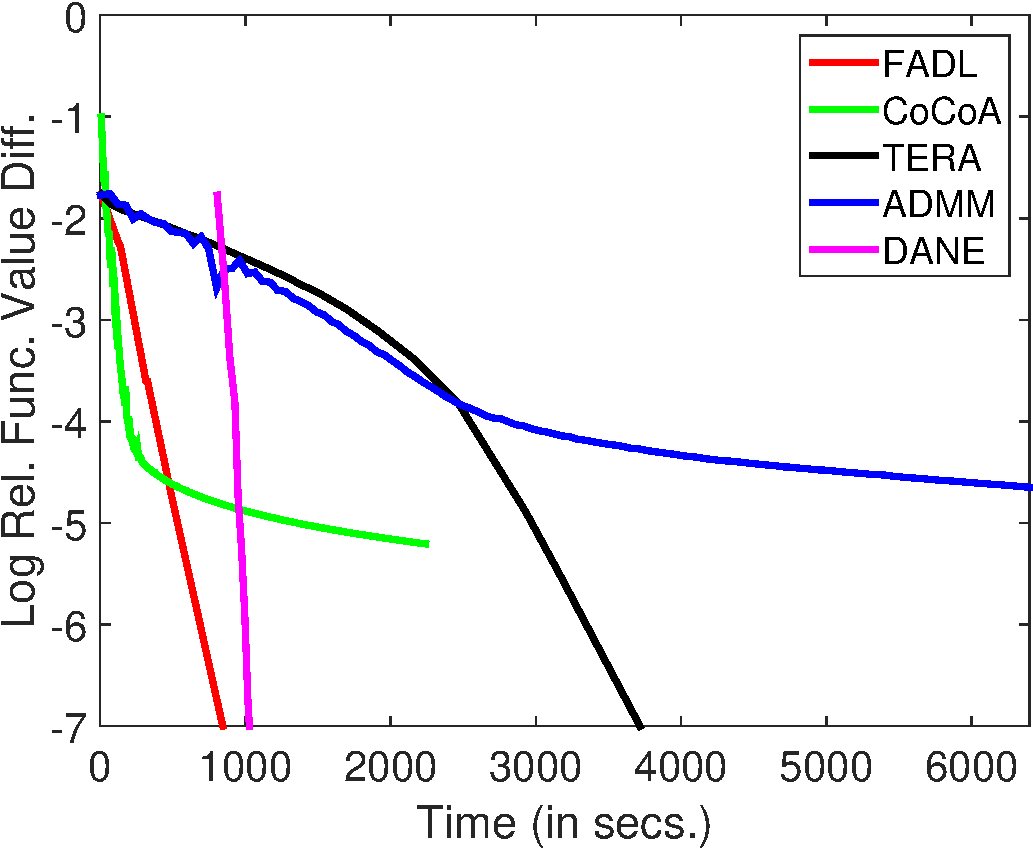
\includegraphics[width=0.46\linewidth]{overallobjvstimeplots/kdd_8-crop}
}
\subfigure[{\it{kdd2010}} - 128 nodes]{
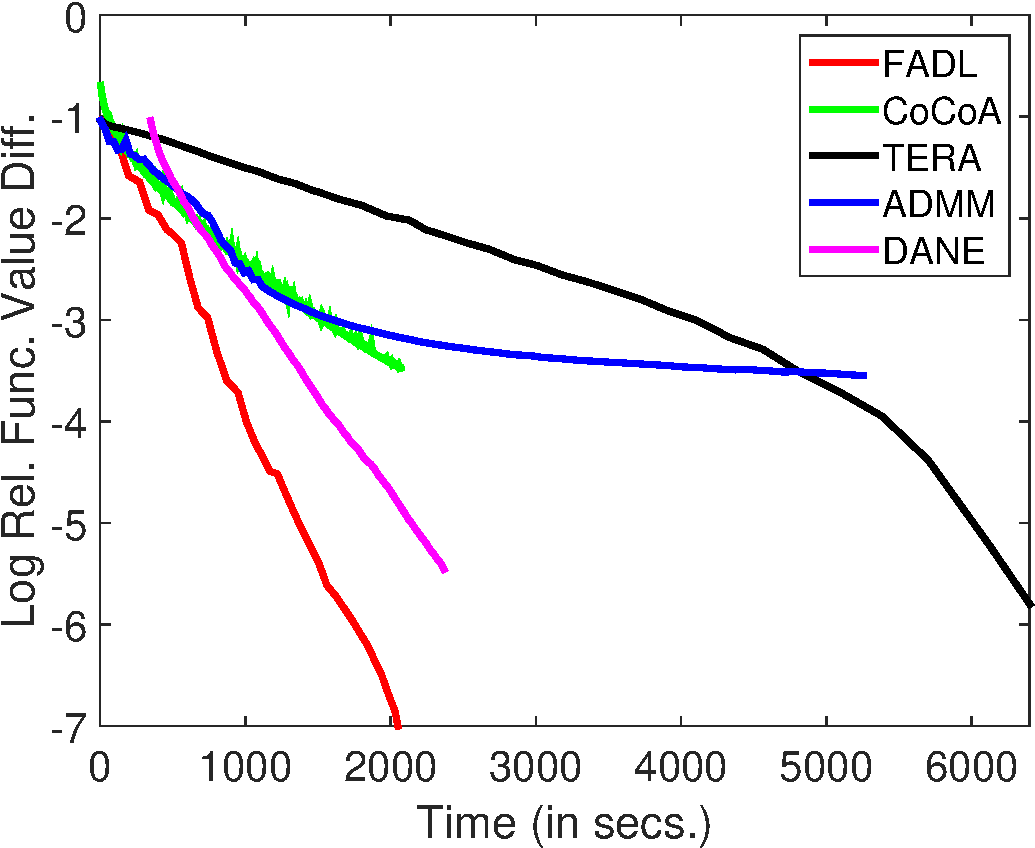
\includegraphics[width=0.46\linewidth]{overallobjvstimeplots/kdd_128-crop}
}

\subfigure[{\it{url}} - 8 nodes]{
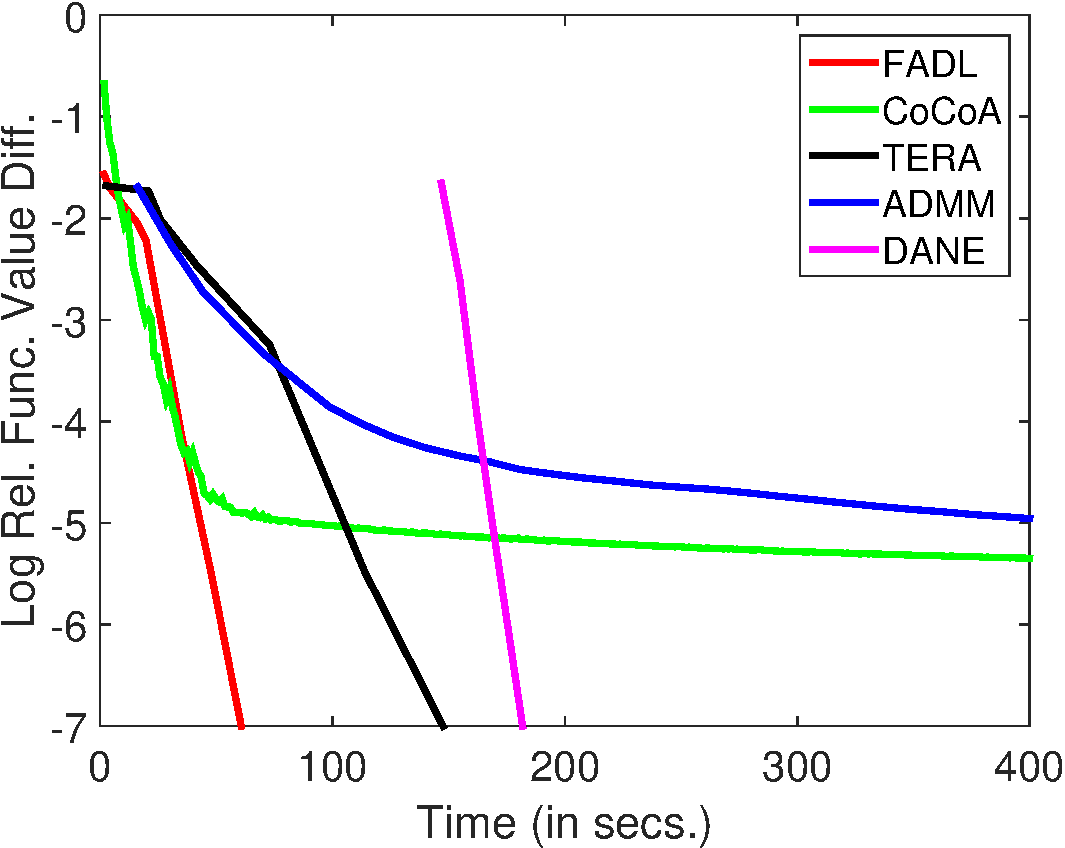
\includegraphics[width=0.46\linewidth]{overallobjvstimeplots/url_8-crop}
}
\subfigure[{\it{url}} - 128 nodes]{
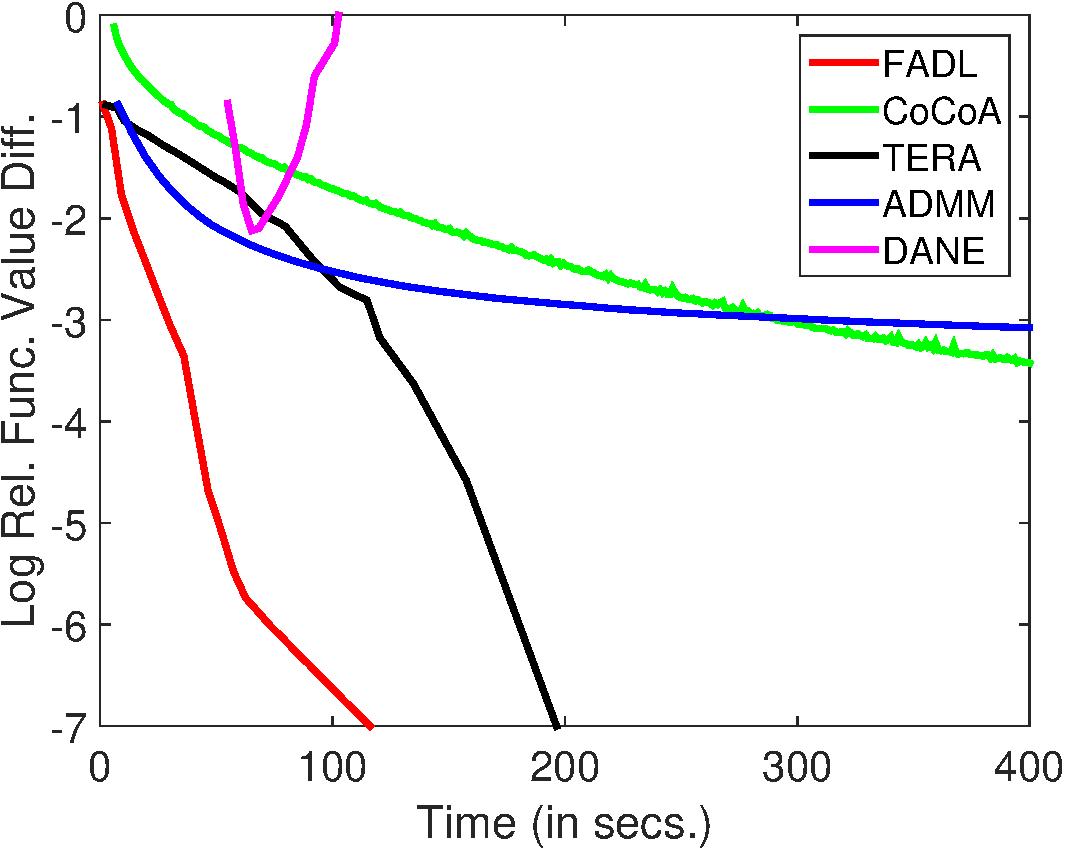
\includegraphics[width=0.46\linewidth]{overallobjvstimeplots/url_128-crop}
}

\subfigure[{\it{webspam}} - 8 nodes]{
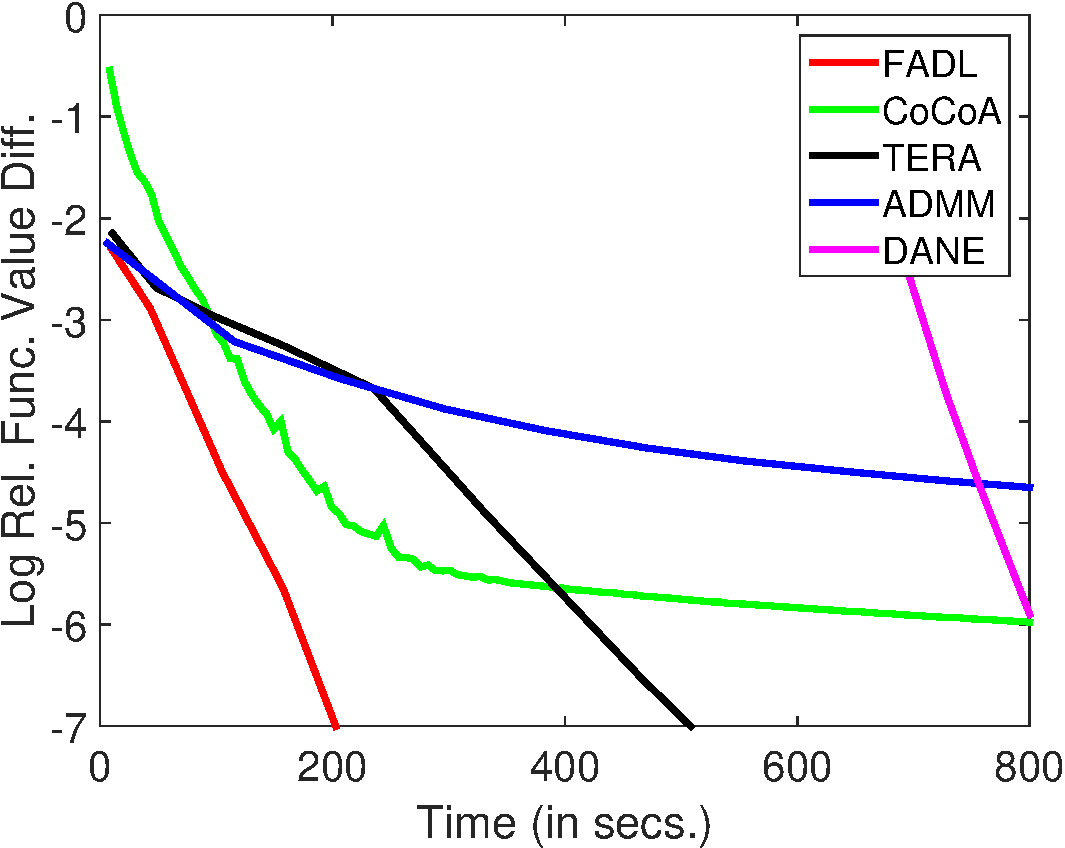
\includegraphics[width=0.46\linewidth]{overallobjvstimeplots/webspam_8-crop}
}
\subfigure[{\it{webspam}} - 128 nodes]{
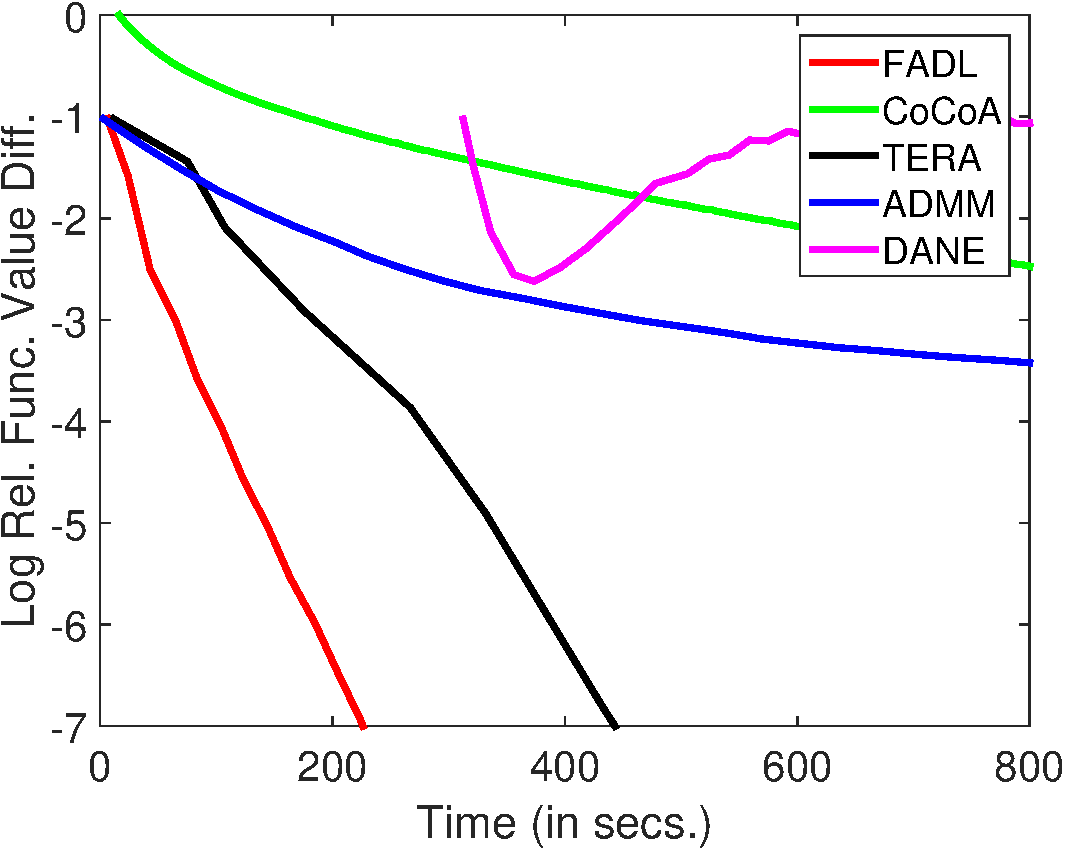
\includegraphics[width=0.46\linewidth]{overallobjvstimeplots/webspam_128-crop}
}

\caption{Plots showing the time efficiency of various methods for the three high dimensional datasets.}
\label{fig:timepass1}
\end{figure}

\begin{figure}[H]
\centering

\subfigure[{\it{mnist8m}} - 8 nodes]{
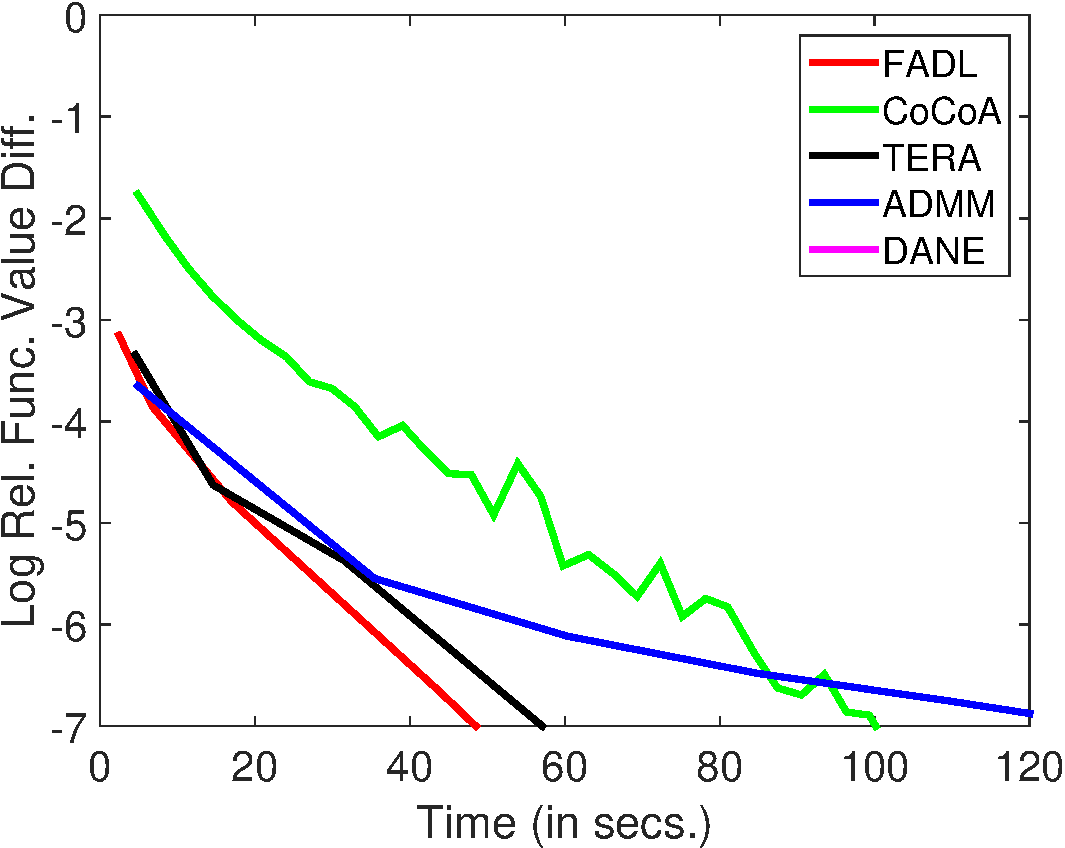
\includegraphics[width=0.46\linewidth]{overallobjvstimeplots/mnist_8-crop}
}
\subfigure[{\it{mnist8m}} - 128 nodes]{
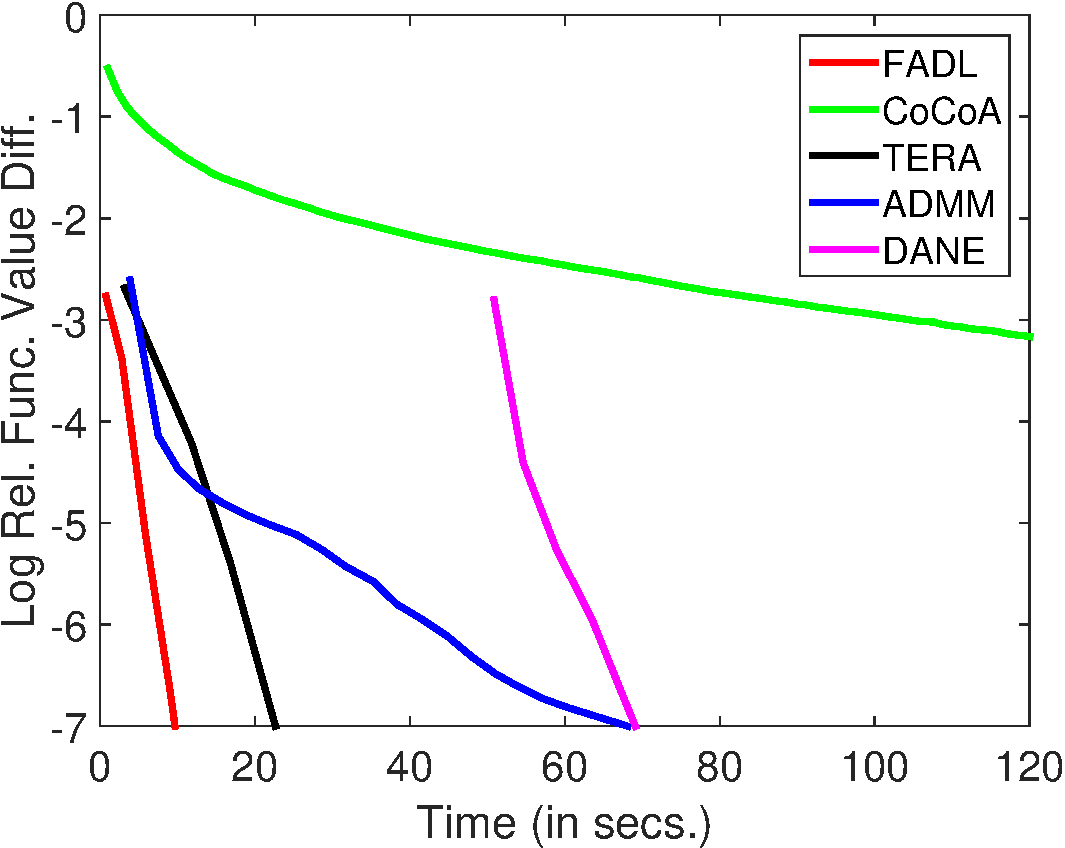
\includegraphics[width=0.46\linewidth]{overallobjvstimeplots/mnist_128-crop}
}

\subfigure[{\it{rcv}} - 8 nodes]{
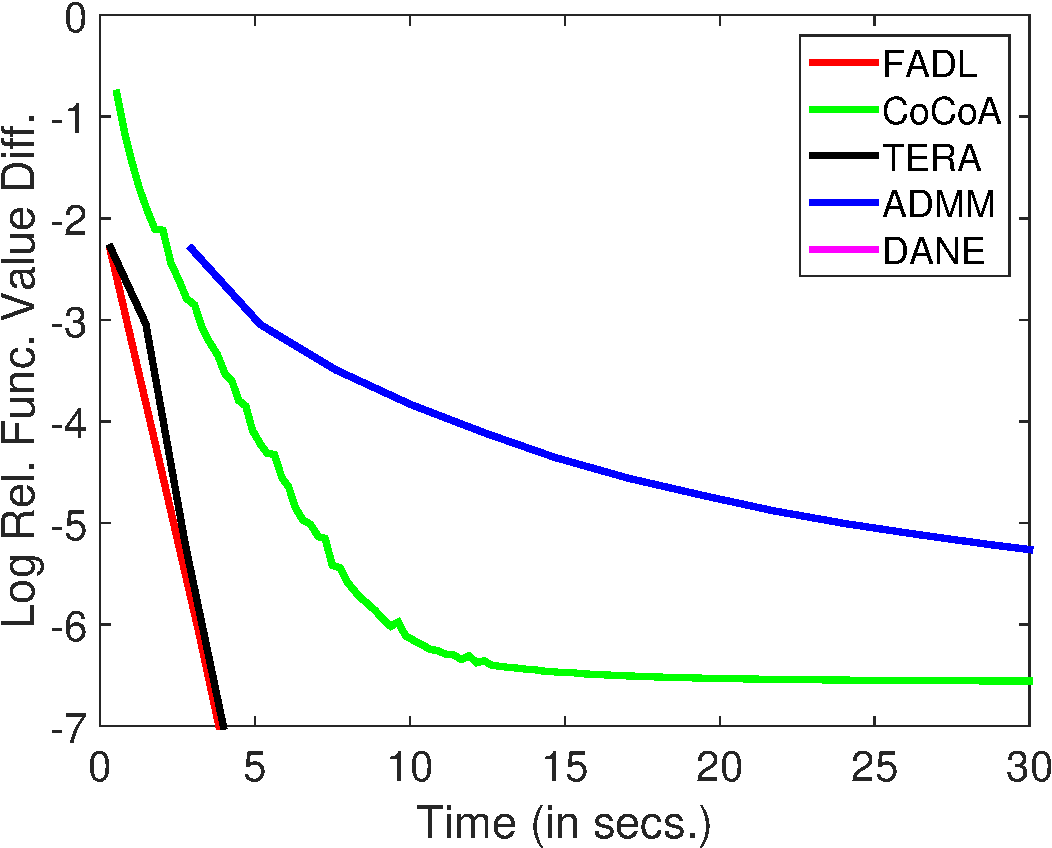
\includegraphics[width=0.46\linewidth]{overallobjvstimeplots/rcv_8-crop}
}
\subfigure[{\it{rcv}} - 128 nodes]{
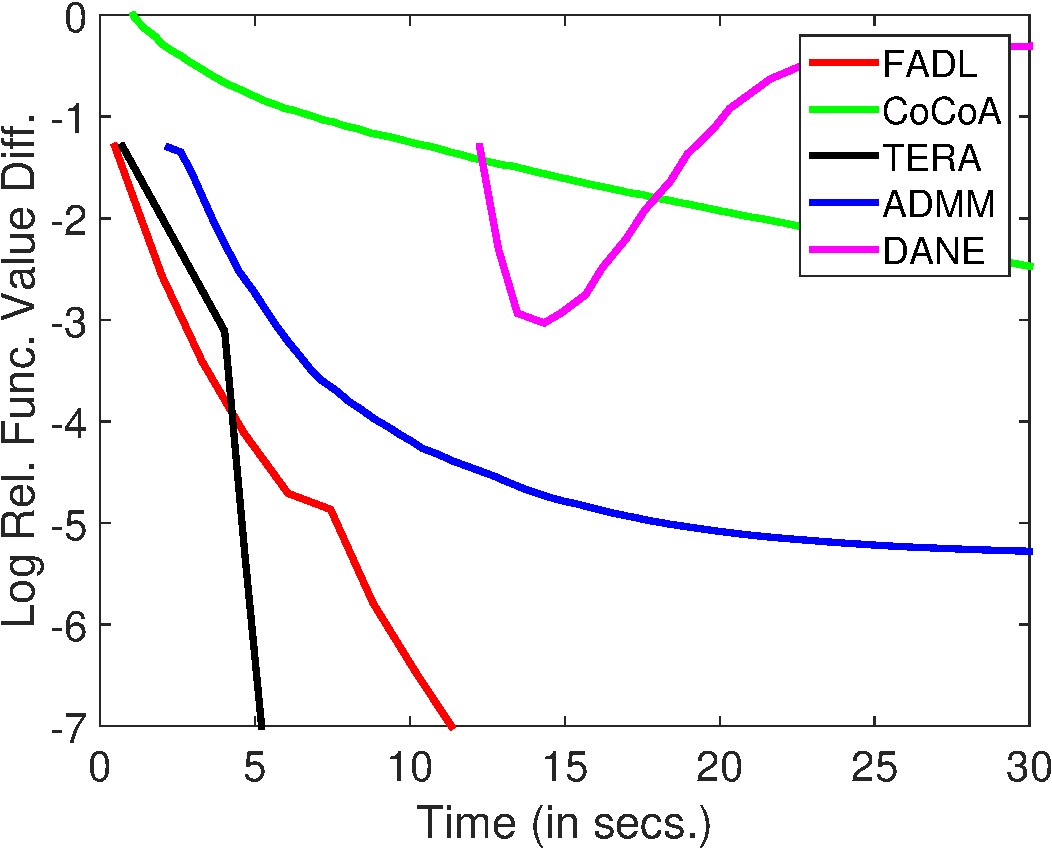
\includegraphics[width=0.46\linewidth]{overallobjvstimeplots/rcv_128-crop}
}

\caption{Plots showing the time efficiency of various methods for the two low/medium dimensional datasets. For {\it{rcv}} and {\it{mnist8m}} - 8 nodes, the plot of DANE is invisible since the time taken for tuning $\mu$ is larger than the time window displayed.}
\label{fig:timepass2}
\end{figure}

\subsubsection{Relative performance of the methods}
\label{subsubsec:relative}

Figure~\ref{fig:auprctime} is relevant for this study.
CoCoA shows impressive speed-up over TERA on {\it kdd2010} but it is much slower on all the other datasets. It is unclear why CoCoA fares so well on {\it kdd2010} but not on the other datasets. ADMM gives an overall decent performance when compared to TERA. FADL is consistently faster than TERA, with speed-ups ranging anywhere from 1-10. In communication-heavy scenarios where reducing the number of communication passes is most important, methods such as FADL and ADMM have great value (see Figure~\ref{fig:auprcpass}), with the possibility of getting even higher speed-ups over TERA. Except for {\it kdd2010} for which FADL is slower than CoCoA for small number of nodes, it is generally the fastest method. DANE does not seem to have any special scenario where it is better than others.

\begin{figure}[H]
\centering

\subfigure[kdd2010]{
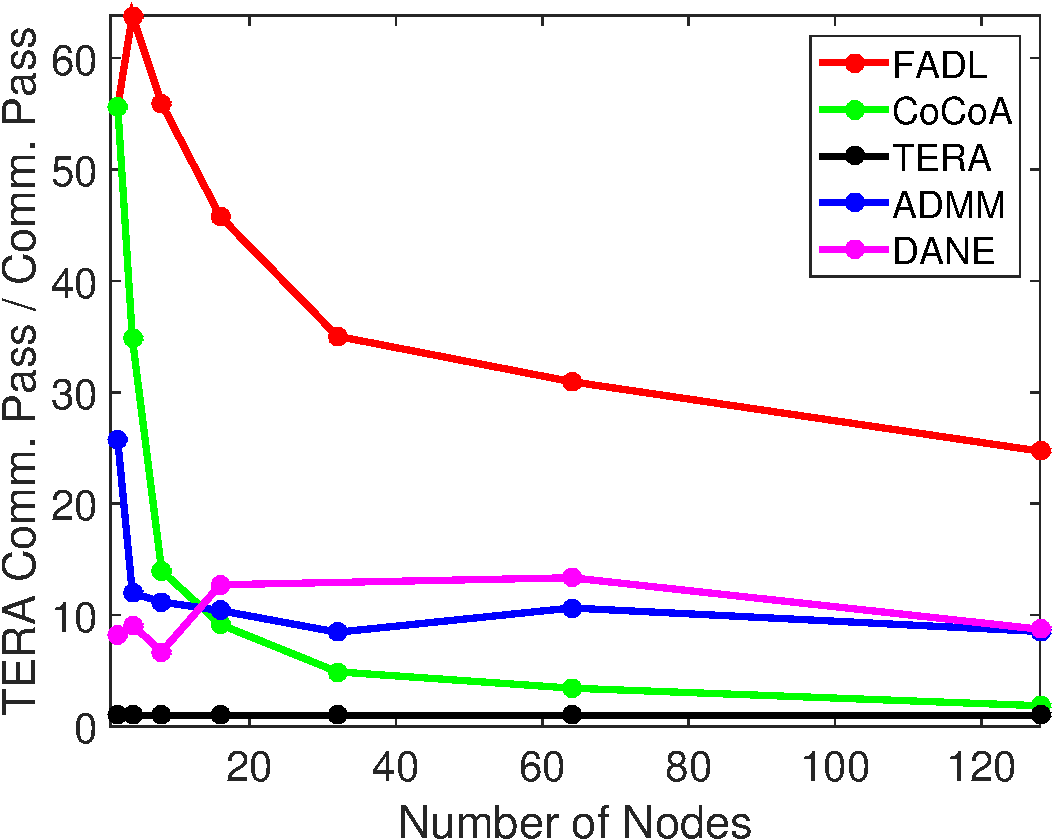
\includegraphics[width=0.46\linewidth]{overallcommpassvsnodesplotsauprcbased/kdd-crop}
}
\subfigure[url]{
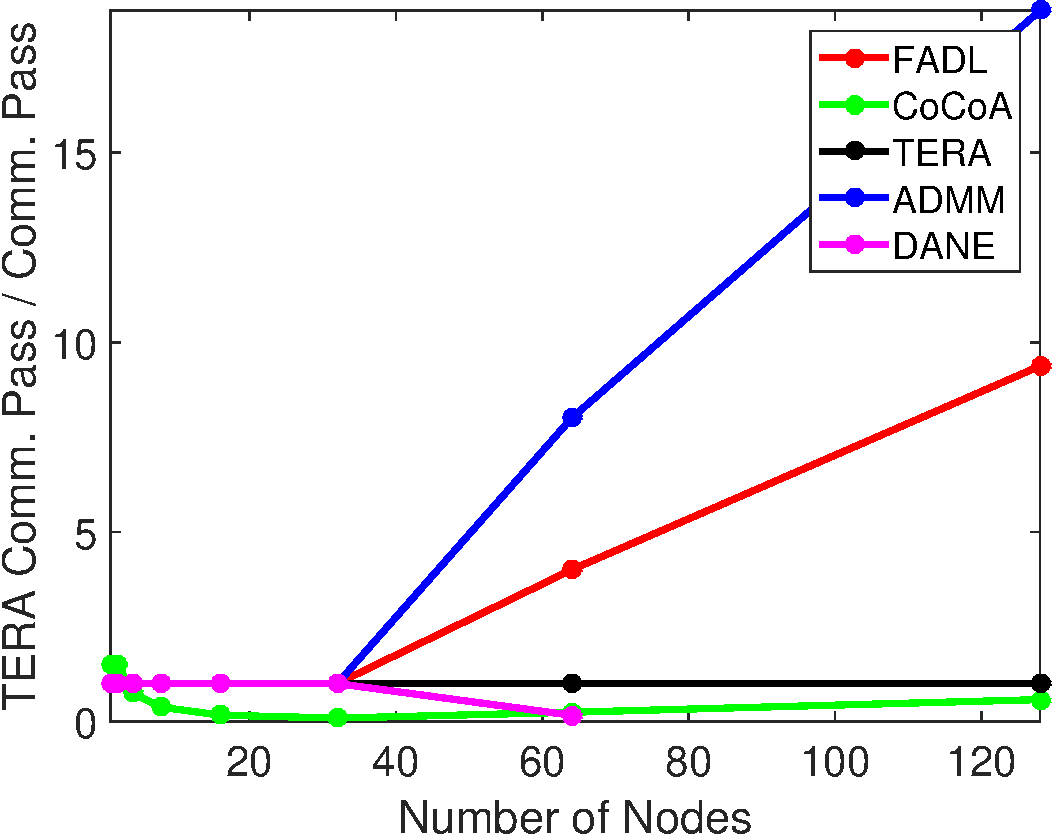
\includegraphics[width=0.46\linewidth]{overallcommpassvsnodesplotsauprcbased/url-crop}
}

\subfigure[webspam]{
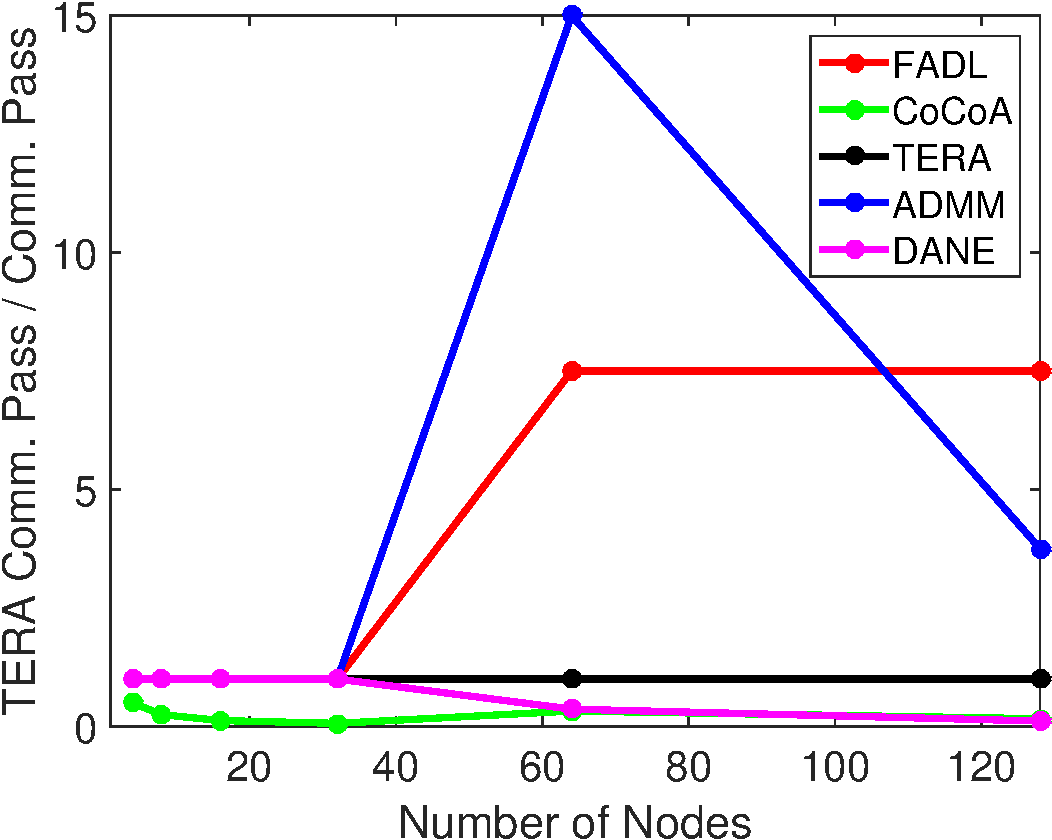
\includegraphics[width=0.46\linewidth]{overallcommpassvsnodesplotsauprcbased/webspam-crop}
}
\subfigure[mnist8m]{
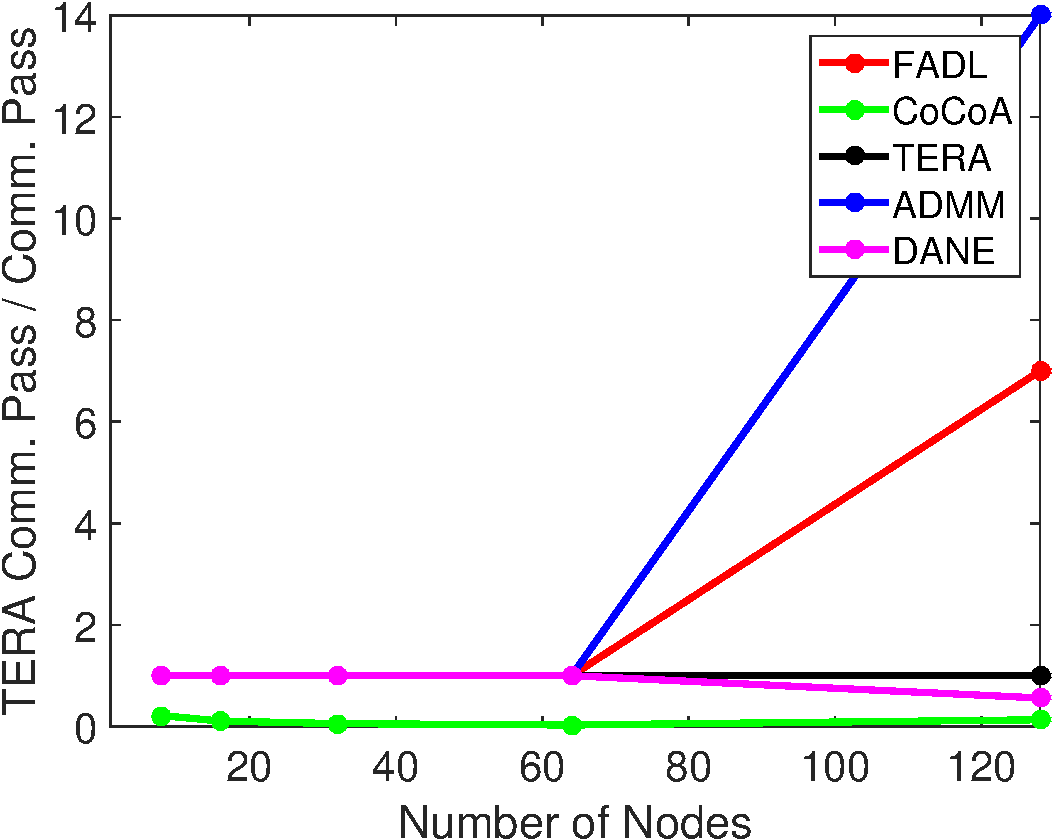
\includegraphics[width=0.46\linewidth]{overallcommpassvsnodesplotsauprcbased/mnist-crop}
}

\subfigure[rcv]{
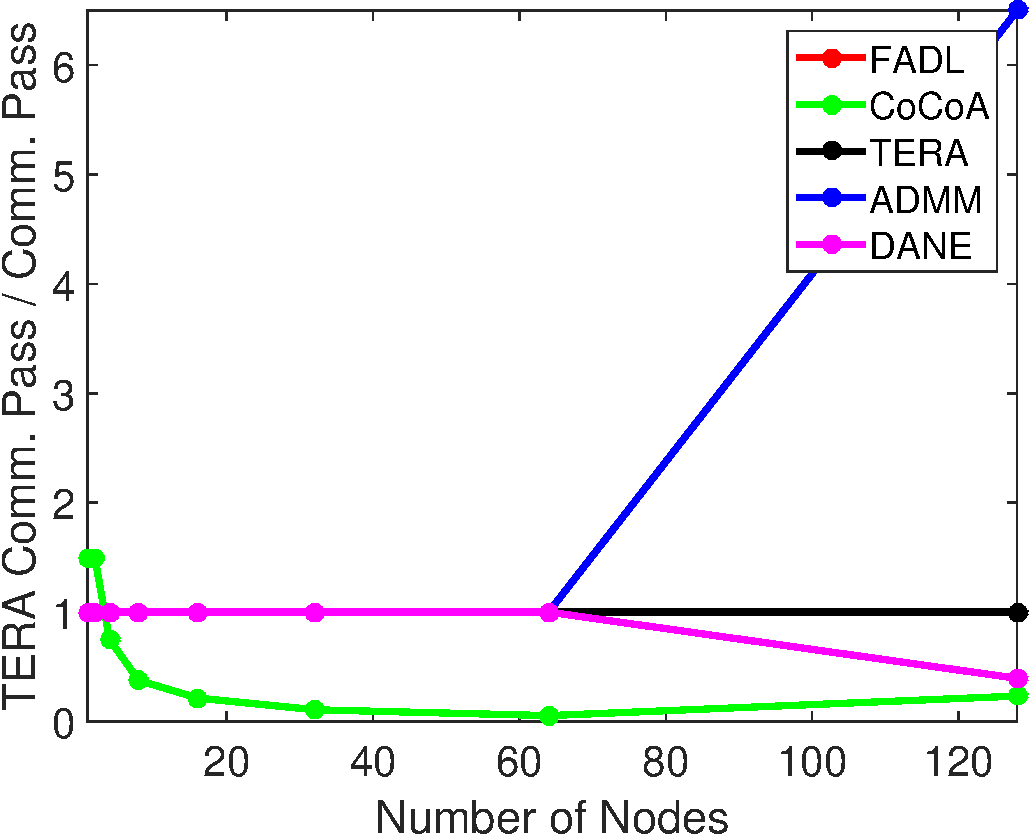
\includegraphics[width=0.46\linewidth]{overallcommpassvsnodesplotsauprcbased/rcv-crop}
}

\caption{Plots showing communication passes (relative to TERA) as a function of the number of nodes. Each method was terminated when it reached within 0.1\% of the steady state AUPRC value achieved by full, perfect training of~(\ref{risk}). For {\it rcv}, the FADL and ADMM curves coincide.}
\label{fig:auprcpass}
\end{figure}


\begin{figure}[H]
\centering

\subfigure[kdd2010]{
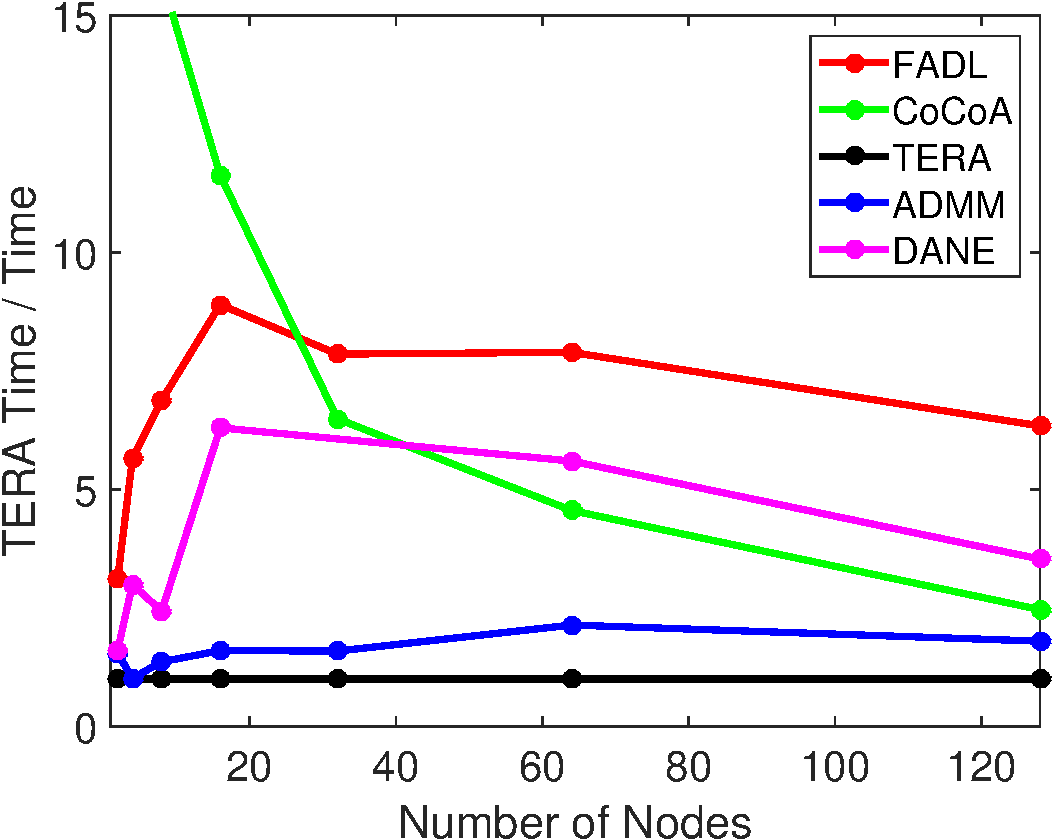
\includegraphics[width=0.46\linewidth]{overallauprcvsnodesplots/kdd-crop}
}
\subfigure[url]{
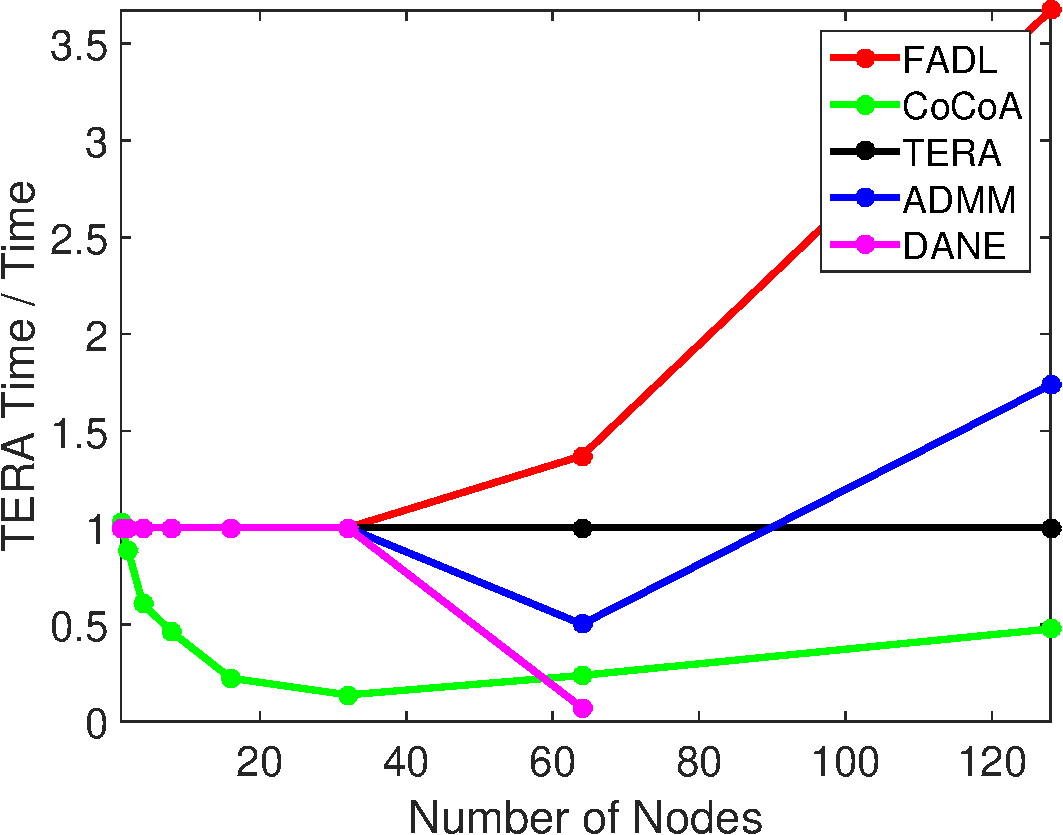
\includegraphics[width=0.46\linewidth]{overallauprcvsnodesplots/url-crop}
}

\subfigure[webspam]{
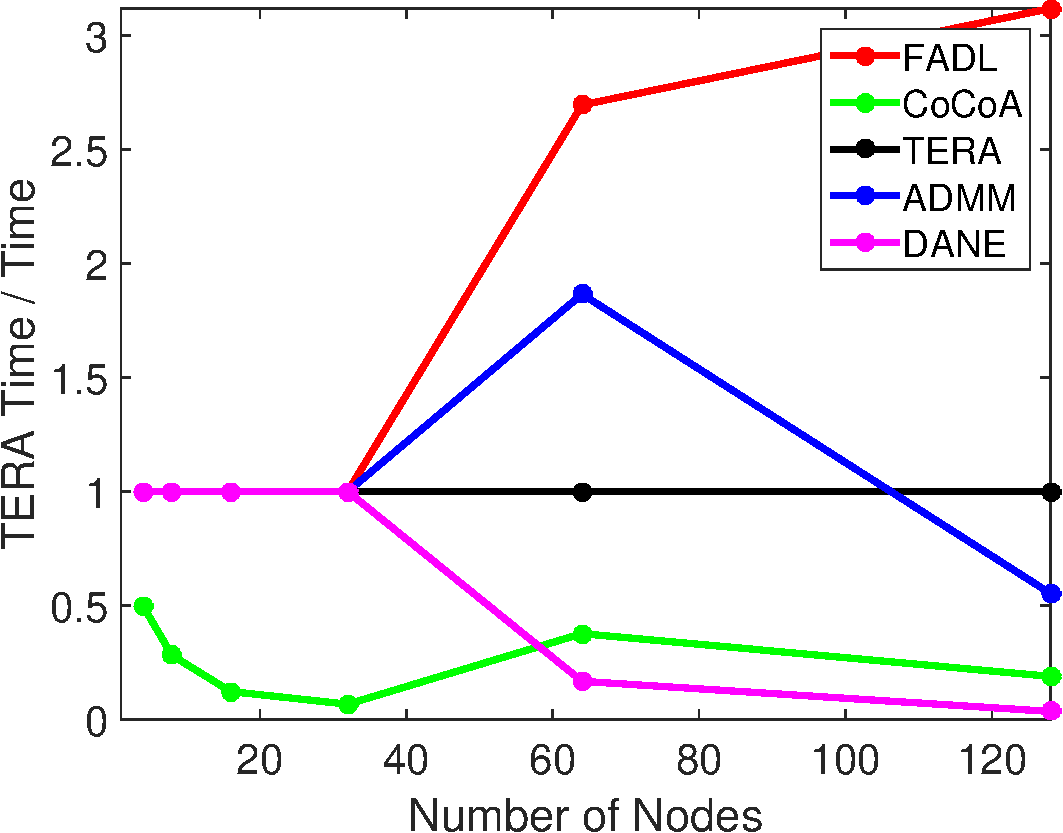
\includegraphics[width=0.46\linewidth]{overallauprcvsnodesplots/webspam-crop}
}
\subfigure[mnist8m]{
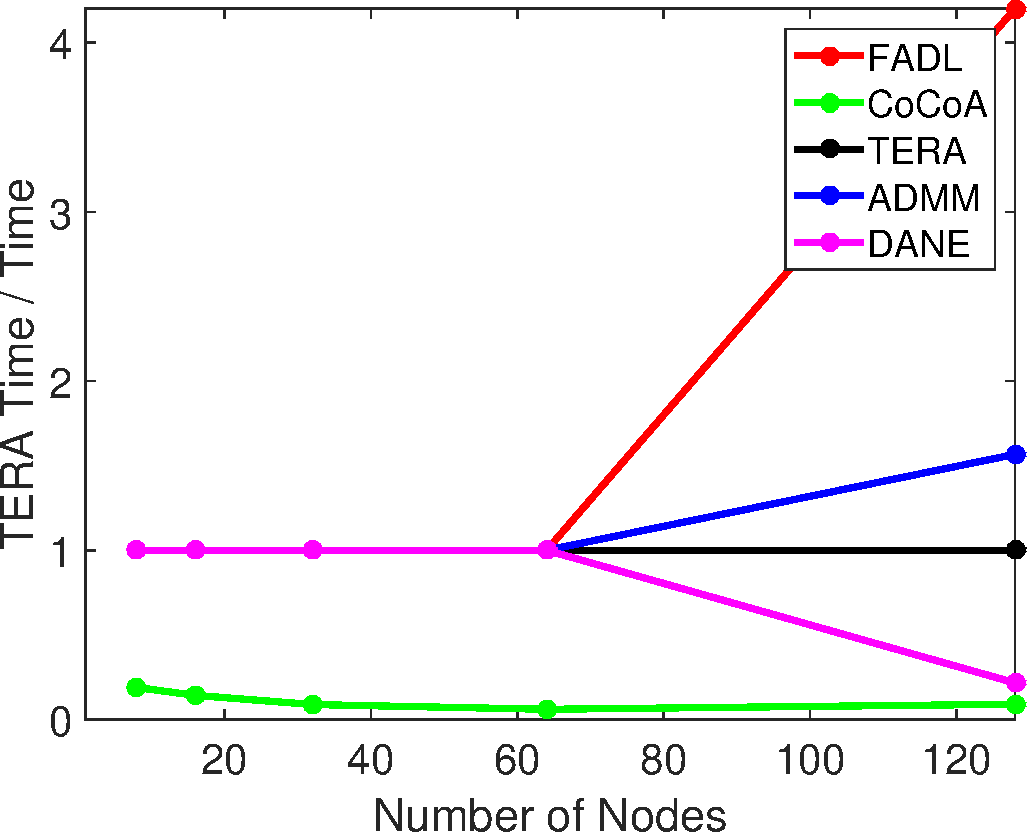
\includegraphics[width=0.46\linewidth]{overallauprcvsnodesplots/mnist-crop}
}

\subfigure[rcv]{
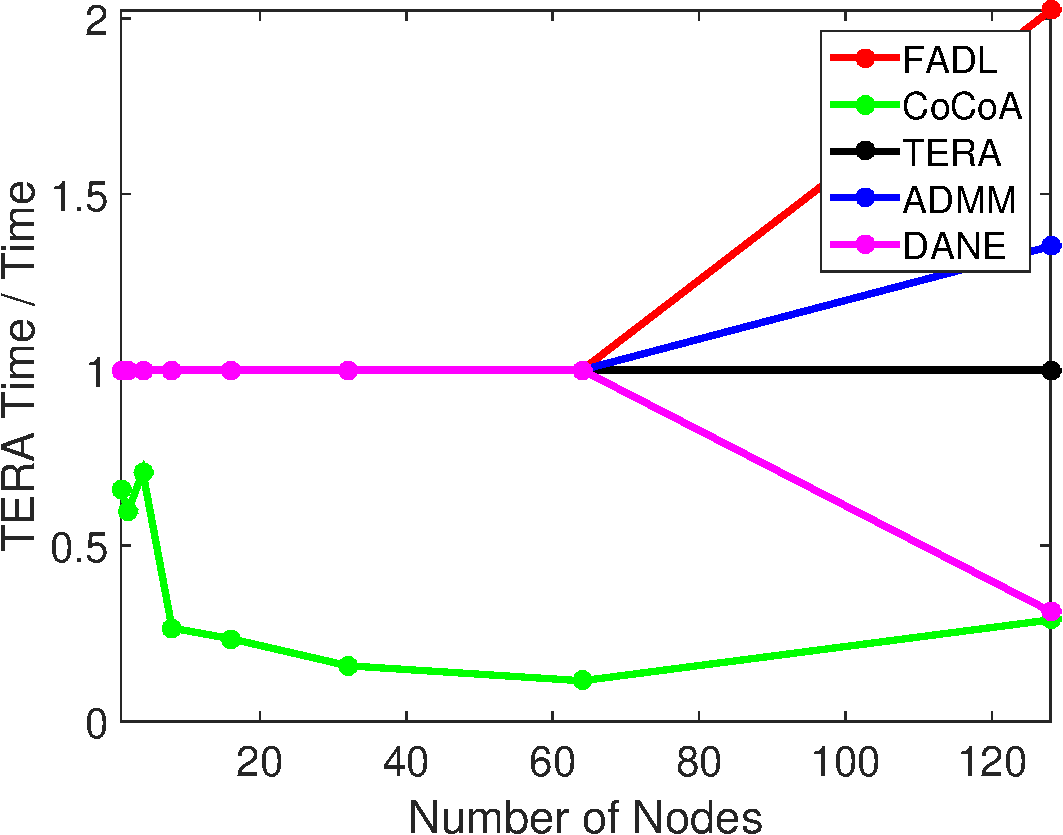
\includegraphics[width=0.46\linewidth]{overallauprcvsnodesplots/rcv-crop}
}

\caption{Plots showing time (relative to TERA) as a function of the number of nodes. Each method was terminated when it reached within 0.1\% of the steady state AUPRC value achieved by full, perfect training of~(\ref{risk}).}
\label{fig:auprctime}
\end{figure}

\subsubsection{Speed-up as a function of $P$}
\label{subsubsec:speedup}

Let us revisit Figure~\ref{fig:timepass1} and look at the plots corresponding to {\it kdd2010} for FADL.\footnote{We choose FADL as an example, but the comments made in the discussion apply to other methods too.} It can be observed that the time needed for reaching a certain tolerance, say {\it Log Rel. Func. Value Diff. = -3}, is two times smaller for $P=8$ than for $P=128$. This means that using a large number of nodes is not useful, which prompts the question: {\it Is a distributed solution really necessary?} There are two answers to this question. First, as we already mentioned, when the training data is huge\footnote{The datasets, {\it kdd2010}, {\it url} and {\it webspam} are really not huge in the {\it Big data} sense. In this paper we used them only because of lack of availability of much bigger public datasets.} and {\it the data is generated and forced to reside in distributed nodes (moving data between machines is not an efficient option)}, the right question to ask is not whether we get great speed-up, but to ask which method is the fastest. Second, for a given dataset and method, if the time taken to reach a certain approximate stopping tolerance (e.g., based on AUPRC) is plotted as a function of $P$, it usually has a minimum at a value $P>1$. Given this, it is appropriate to choose a $P$ optimally to minimize training time. A large fraction of Big data machine learning applications involve periodically repeated model training involving newly added data. For example, in Advertising, logistic regression based click probability models are retrained on a daily basis on incrementally varying datasets. In such scenarios it is worthwhile to spend time to tune $P$ in an early deployment phase to minimize time, and then use this choice of $P$ for future runs.

\subsubsection{Computation and Communication Costs}
\label{subsubsec:costs}

Table~\ref{tab:compcommcost} shows the ratio of computational cost to communication cost for the three high dimensional datasets for all the methods.\footnote{For the medium/low dimensional datasets {\it rcv} and {\it mnist8m}, communication latencies, line search cost etc. also play a key role and an analysis of computation cost versus communication cost does not provide any great insight.}
Note that the ratio is small for {\it TERA} and so communication cost dominates the time for it. On the other hand, both the costs are well balanced for FADL. Note that ratio varies in the range of $0.625-2.845$. This clearly shows that FADL trades-off computation with communication, while significantly reducing the number of communication passes (Figures~\ref{fig:commpass1} and~\ref{fig:commpass2}) and time (Figures~\ref{fig:timepass1} and~\ref{fig:timepass2}).


%We also notice that the gap between our methods and {\it{SQM}} and {\it{HYBRID}} decreases with increasing number of nodes. This happens because our functional approximation becomes cruder as $P$ increases. The exact $P$ up to which our approach performs better varies from dataset to dataset and depends on the learning curve. For steeper learning curves, our performance should degrade slower. The exact analysis is left as a future work. Similar observations can be made on the time curves in Figure~\ref{}.

%Finally, Figure~\ref{} shows time versus AUPRC results for different methods. Our method clearly outperforms both {\it{HYBRID}} and {\it{SQM}} in getting good AUPRC values (within $0.5\%$ of the optimal).

%To conclude, our functional approximation based distributed learning algorithm is flexible and fills several gaps in the literature. We have demonstrated that our algorithms work well when (a) the number of features is very large, (b) the functional approximation is good, and (c) moderately small relative objective function error is desired. We expect to come up with better functional approximations and hybrid algorithms in the near future that does well under all conditions.



\begin{table}[ht]
\centering % used for centering table
\begin{tabular}{|c|c|c|c|c|c} % centered columns (4 columns)
\hline %inserts double horizontal lines
& FADL & CoCoA & TERA & ADMM  \\
\hline
{\it kdd2010} & 1.6333 &   0.1416  &   0.1422  &  1.8499\\
\hline
{\it url} & 1.3650 &   0.1040  &  0.2986 &    3.4886\\
\hline
{\it webspam} & 1.2082 &   0.1570  &  0.2423 &    1.2543\\
%\hline
%{\it mnist8m} & 0.7942 &   0.1385 &   1.5486 &    5.7881\\
%\hline
%{\it rcv}   &  0.9693  &  0.0486  &  3.6671  &  1.6682 \\
\hline
\end{tabular}
\caption{Ratio of the total computation cost to the total communication cost for various methods which were terminated when AUPRC reached within 0.1\% of the AUPRC value for 128 nodes.} % title of Table
\label{tab:compcommcost}
\end{table}

\subsection{Experiment on a much larger dataset}
\label{subsec:splice}

To verify the goodness of FADL, we also did an experiment evaluating FADL against other methods, on a large dataset that is more than an order of magnitude bigger than the largest dataset in Table~\ref{tab:params}. The dataset is the Splice site recognition dataset from the bioinformatics domain~\citep{sonnenburg2010}. In this dataset each example is a sequence; we considered all positional features upto 9 grams. This led to a dataset of 49 million features and 50 million examples. The size of the dataset is larger than 0.65 Terabytes. We employed a cluster of 100 nodes to solve this problem. Figure~\ref{fig:splice} compares the various methods on (a) the reduction of the objective function as a function of communication passes; (b) the reduction of the objective function as a function of time; and (c) the improvement of generalization performance (AUPRC) as a function of time. It is clear that FADL makes great reductions over other methods, on the number of communication passes. FADL is also the best performer when we measure by the time taken. On clusters with slower communication speeds and iteration set-up times, the value of FADL over other methods will be even higher. Interestingly, CoCoA comes out as the next best performer. CoCoA has slower end convergence than FADL, but it shows up equally well in plot (c) on the improvement of generalization performance. As we saw earlier with other datasets, the value of CoCoA varies a lot; for the current scenario of solving the splice site recognition on 100 nodes it seems to be well-suited. FADL, on the other hand, is uniformly good in varying scenarios of several datasets, number of nodes etc.

\begin{figure}[t]
\centering

\subfigure[Communication efficiency (objective function)]{
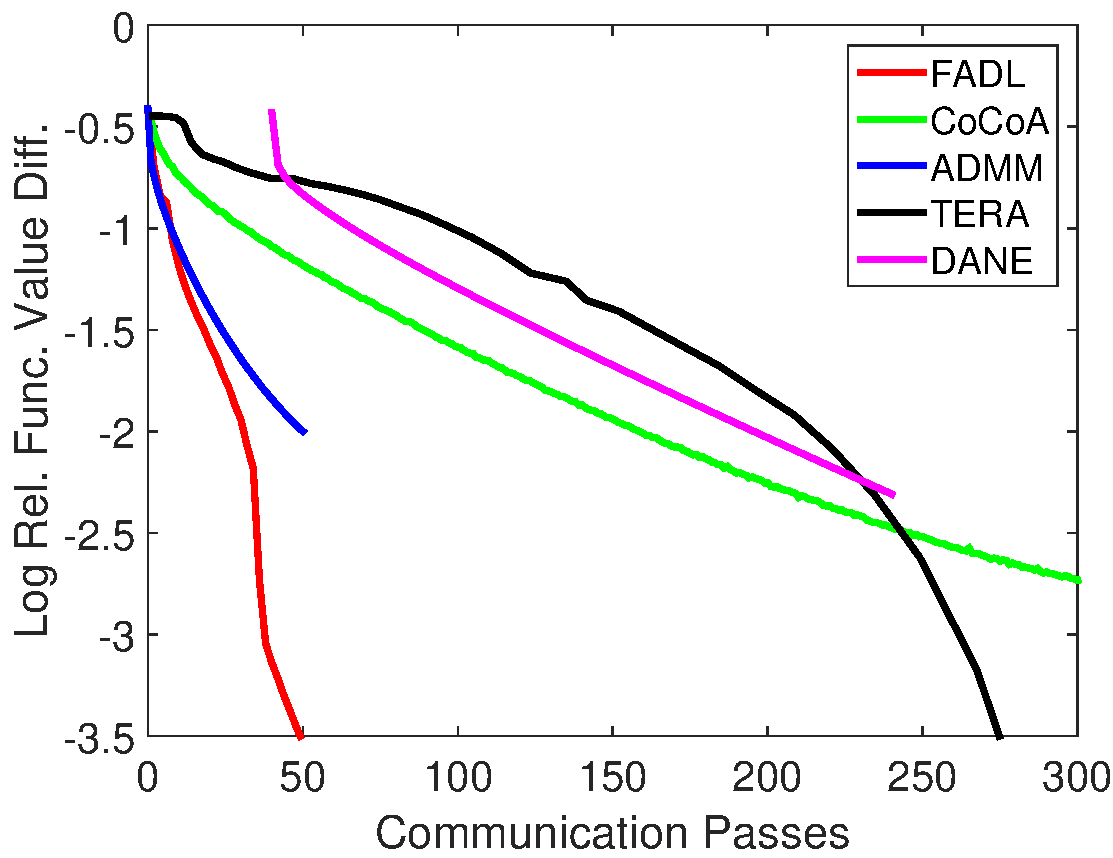
\includegraphics[width=0.46\linewidth]{splice/splicefuncvscommpass}
}
\subfigure[Time efficiency (objective function)]{
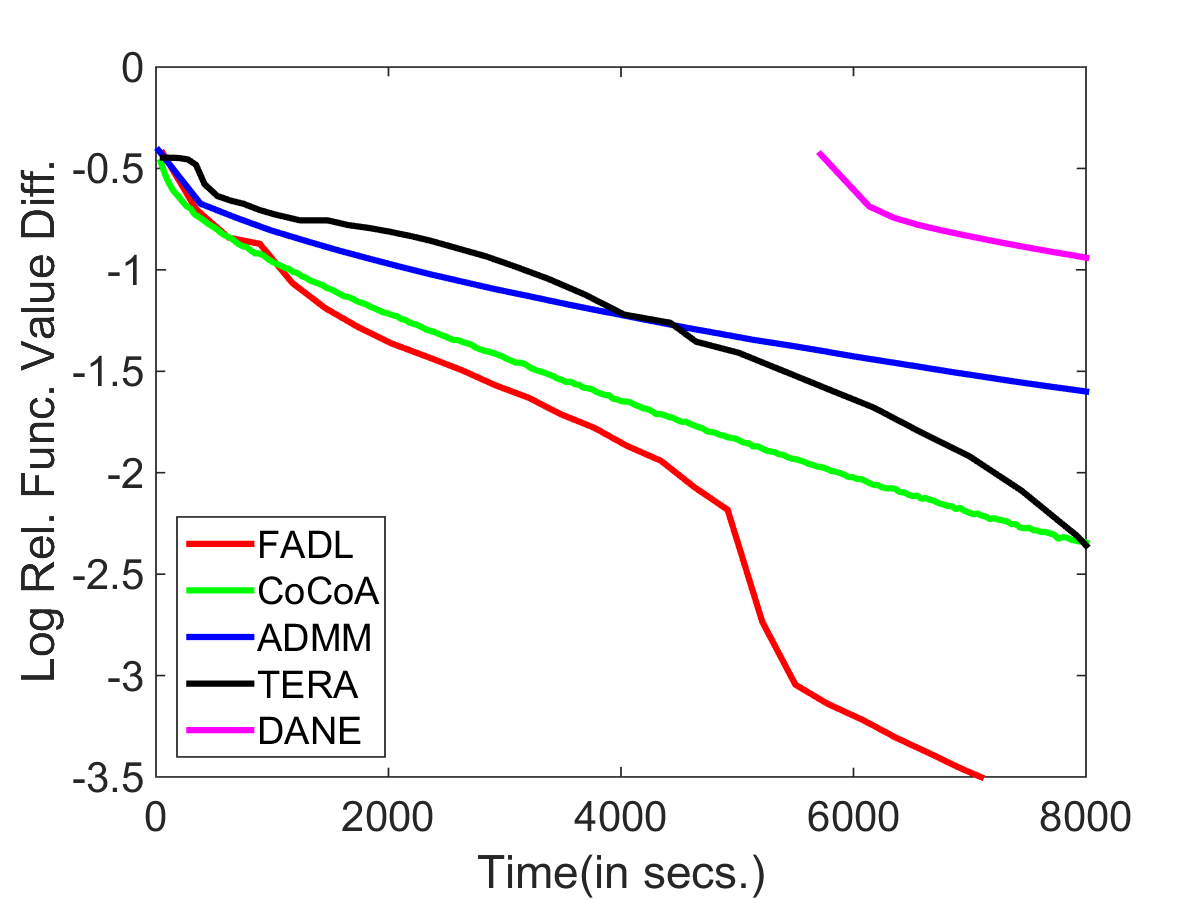
\includegraphics[width=0.46\linewidth]{splice/splicefuncvstime}
}
\subfigure[Time efficiency (AUPRC)]{
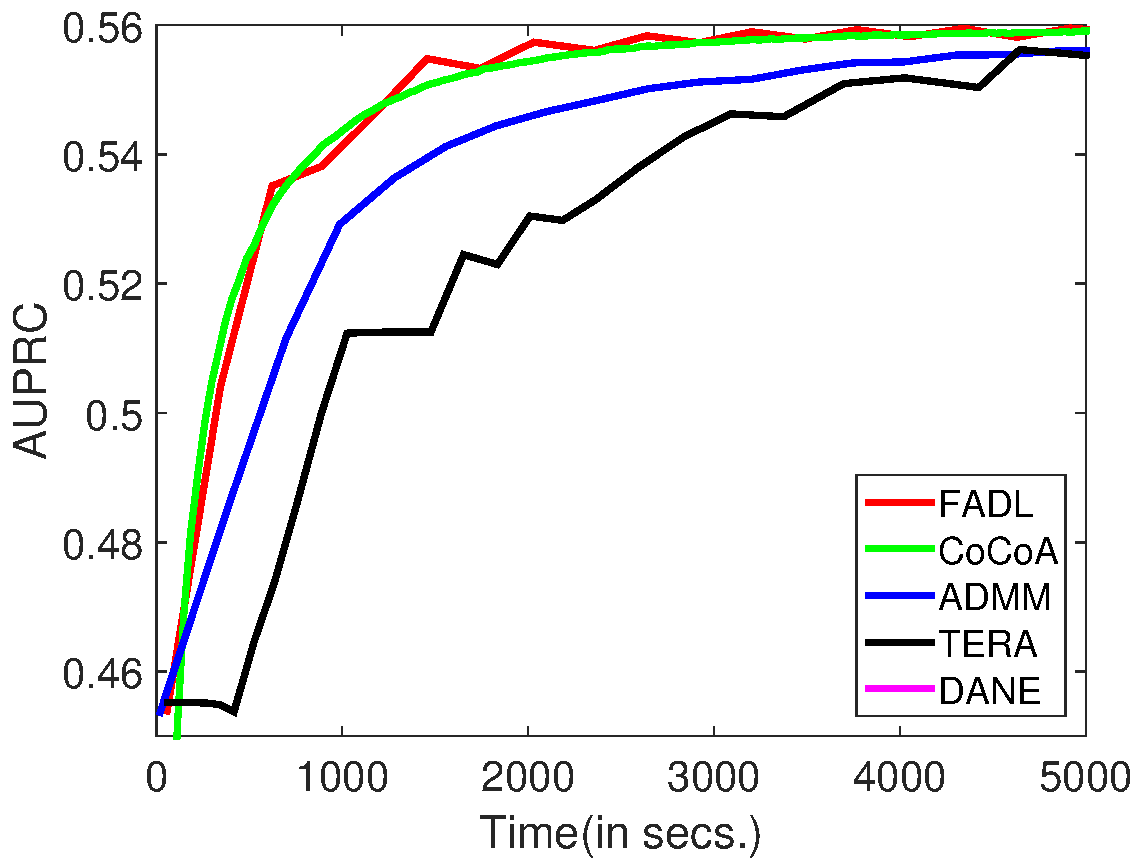
\includegraphics[width=0.46\linewidth]{splice/spliceaccvstime}
}

\caption{Plots comparing various methods on the {\it Splice site recognition} dataset.}
\label{fig:splice}
\end{figure}



\subsection{Summary}
\label{subsec:summary}

It is useful to summarize the findings of the empirical study.
\begin{itemize}
\item FADL gives a great reduction in the number of communication passes, making it clearly superior to other methods in communication heavy settings.
\item In spite of higher computational costs per iteration FADL shows the overall best performance on the total time taken. This is true even for medium and low dimensional datasets.
\item FADL shows a speed-up of 1-10 over TERA, the actual speed-up depending on the dataset and the setting.
\item FADL nicely balances computation and communication costs.
\end{itemize}







%\input{relatedwork}
%\input{discussion}

\section{Discussion}
\label{disc}

In this section, we discuss briefly, other different distributed settings made possible by our algorithm. The aim is to show the flexibility and generality of our approach while ensuring {\it glrc}.\comment{ We will also talk briefly about the extension to non-convex setting.}

Section~\ref{distr} considered example partitioning where examples are distributed across the nodes. First, it is worth mentioning that, due to the gradient consistency condition, {\it partitioning} is not a necessary constraint; our theory allows examples to be resampled, i.e., each example is allowed to be a part of any number of nodes arbitrarily. For example, to reduce the number of outer iterations, it helps to have more examples in each node.

Second, the theory proposed in Section~\ref{distr} holds for feature partitioning also. Suppose, in each node $p$ we restrict ourselves to a subset of features, $J_p\subset \{1,\ldots,d\}$, i.e., include the constraint,
$w_p \in  \{ w: w(j)=w^r(j) \;\; \forall r\not\in J_p\}$,
where $w(j)$ denotes the weight of the $j^{th}$ feature. Note that we do not need $\{J_p\}$ to form a partition. This is useful since important features can be included in all the nodes.

\noindent {\bf Gradient sub-consistency.} Given $w^r$ and $J_p$ we say that $\fhat_p(w)$ has gradient sub-consistency with $f$ at $w^r$ on $J_p$ if $\frac{\partial f}{\partial w(j)} (w^r) = \frac{\partial \fhat}{\partial w(j)} (w^r) \;\; \forall \; j\in J_p$.

Under the above condition, we can modify the algorithm proposed in Section~\ref{distr} to come up with a feature decomposition algorithm with {\it glrc}.

Several feature decomposition based approaches~\citep{richtarik2013,patriksson1998fp} have been proposed in the literature. The one closest to our method is the work by Patrikkson on a synchronized parallel algorithm~\citep{patriksson1998fp} which extends a generic cost approximation algorithm~\citep{patriksson1998ca} that is similar to our functional approximation. The sub-problems on the partitions are solved in parallel. Although the objective function is not assumed to be convex, the cost approximation is required to satisfy a monotone property, implying that the approximation is convex. The algorithm only has asymptotic linear rate of convergence and it requires the feature partitions to be disjoint. In contrast, our method has {\it glrc} and works even if features overlap in partitions. Moreover, there does not exist any counterpart of our example partitioning based distributed algorithm discussed in Section~\ref{distr}.

Recently~\citet{mairal2013} has developed an algorithm called MISO. The main idea of MISO (which is in the spirit of the EM algorithm) is to build majorization approximations with good properties so that line search can be avoided, which is interesting. MISO is a serial method. Developing a distributed version of MISO is an interesting future direction; but, given that line search is inexpensive communication-wise, it is unclear if such a method would give great benefits.

Our approach can be easily generalized to joint example-feature partitioning as well as non-convex settings.\footnote{For non-convex settings {\it glrc} is hard to establish, but proving a simpler convergence theory is quite possible.} The exact details of all the extensions mentioned above and related experiments are left for future work.

%\Kee{Changes have been made below.}

Recently, a powerful divide and conquer approach~\citet{hsieh14} has been suggested for training kernel methods. The idea is to partition the input space such that the restrictions of training on the partitioned input spaces are as decoupled as possible. If, in FADL, we had the ability to choose the parts of data that are placed in the nodes, then we would also gain by choosing decoupled partitions. However, in the distributed case, this requires pre-processing as well as shuffling of data, which are expensive.

\section{Conclusion}
\label{conc}

To conclude, we have proposed FADL, a novel functional approximation based distributed algorithm with provable global linear rate of convergence. The algorithm is general and flexible in the
sense of allowing different local approximations at the node level, different algorithms for optimizing the local approximation, early stopping and general data usage in the nodes. We also established the superior efficiency of FADL by evaluating it against key existing distributed methods. We believe that FADL has great potential for solving machine learning problems arising in Big data.



%APPENDICES are optional
%\balancecolumns

\appendix

%\input{appendix_B}

\def\C{C}
\def\Ccomp{C^{\rm Comp}}
\def\Ccomm{C^{\rm Comm}}
\def\Csqm{C_{\rm SQM}}
\def\Cfadl{C_{\rm FADL}}
\def\Ccompsqm{C^{\rm Comp}_{\rm SQM}}
\def\Ccommsqm{C^{\rm Comm}_{\rm SQM}}
\def\Ccompfadl{C^{\rm Comp}_{\rm FADL}}
\def\Ccommfadl{C^{\rm Comm}_{\rm FADL}}
\def\Tout{T^{\rm outer}}
\def\Tin{T^{\rm inner}}
\def\Toutsqm{T^{\rm outer}_{\rm SQM}}
\def\Toutour{T^{\rm outer}_{\rm FADL}}

\section*{Appendix A: Complexity analysis}
\label{proofs}
Let us use the notations of section~\ref{distr} given around (\ref{comm}). We define the overall cost of any distributed algorithm as
\begin{eqnarray}
[(c_1\frac{nz}{P} + c_2m)\Tin + c_3 \gamma m]\Tout,
\label{costanal}
\end{eqnarray}
where $\Tout$ is the number of outer iterations, $\Tin$ is the number of inner iterations at each node before communication happens and  $c_1$ and $c_2$ denote the number of passes over the data and $m$-dimensional dot products per inner iteration respectively. For communication, we assume an {\it AllReduce} binary tree as described in~\citet{agarwal2011} with pipelining. As a result, we do not have a multiplicative factor of $log_2 P$ in our cost\footnote{Actually, there is another communication term, $\gamma b\; log_2 P$, where $b$ is the size of first block of communicated doubles in the pipeline. However, typically $b\ll m$ and hence we ignore it.}. $\gamma$ is the relative computation to communication speed in the given distributed system; more precisely, it is the ratio of the times associated with communicating a floating point number and performing one floating point operation; $\gamma$ is usually much larger than $1$.
$c_3$ is the number of $m$-dimensional vectors (gradients, Hessian-vector computations etc.) we need to communicate.

\begin{table}[ht]
\centering % used for centering table
\begin{tabular}{c c c c c c c} % centered columns (4 columns)
\hline\hline %inserts double horizontal lines
Method & $c_1$ & $c_2$ & $c_3$ & $\Tin$ \\ %[0.5ex] % inserts table
%heading
\hline
SQM & $2$ & $\approx 5-10$ & $1$ & $1$ \\
FADL & $2$ & $\approx 5-7$ & $2$ & $\hat{k}$ \\
\hline
\end{tabular}
\caption{Value of cost parameters} % title of Table
\label{tab:costparams}
\end{table}

The values of different parameters for SQM and FADL are given in Table~\ref{tab:costparams}. $\Toutsqm$ is the number of overall conjugate gradient iterations plus gradient computations. $\hat{k}$ is the average number of conjugate gradient iterations (for the inner minimization of $\fhat_p$ using TRON) required per outer iteration in FADL. Typically $\hat{k}$ is between $5$ and $20$.

Since dense dot products are extremely fast $c_2 m$ is small compared to $c_1 nz/P$ for both the approaches, we ignore it from (\ref{costanal}) for simplicity. Now for FADL to have lesser cost than TERA, we can use (\ref{costanal}) to get the condition,
%we need $\Cfadl \leq \Csqm$. Plugging in the parameter values and rearranging,
\begin{equation}
2.0(\hat{k}\Toutour - \Toutsqm)\frac{nz}{P}  \leq  (\Toutsqm - 2 \Toutour) \gamma m
\end{equation}
Let us ignore $\Toutsqm$ on the left side of this inequality (in favor of SQM) and rearrange to get the looser condition,
\begin{equation}
\frac{nz}{m}  \leq  \frac{\gamma P}{\hat{k}} \frac{1}{2.0}(\frac{\Toutsqm}{\Toutour} - 2 )
\end{equation}
Assuming $\Toutsqm > 3.0\Toutour$, we arrive at the final condition in~(\ref{comm}).
%Note that in our experiments (section~\ref{distr}), the savings we get in the outer iterations is typically more than the factor $3.2$.



%\input{appendix_A}
\section*{Appendix B: Proofs}
\label{sec:proofs}

\subsection*{Proofs of the results in section~\ref{general}}

Let us now consider the establishment of the convergence theory given in section~\ref{general}.

\vspace*{0.1in}

\noindent {\bf Proof of Lemma 1.}
Let $\rho(t)=f(w^r+td^r)$ and $\gamma(t)=\rho(t)-\rho(0)-\alpha t\rho^\prime(0)$.
Note the following connections with quantities involved in Lemma 1: $\rho(t)=f^{r+1}$, $\rho(0)=f^r$, $\rho^\prime(t)=g^{r+1}\cdot d^r$ and $\gamma(t)=f^{r+1} - f^r - \alpha g^r\cdot(w^{r+1}-w^r)$.
(\ref{ag}) corresponds to the condition $\gamma(t)\le 0$ and (\ref{wolfe}) corresponds to the condition $\rho^\prime(t)\ge \beta\rho^\prime(0)$.

$\gamma^\prime(t) = \rho^\prime(t)-\alpha \rho^\prime(0)$.
$\rho^\prime(0)<0$.
$\rho^\prime$ is strictly monotone increasing because, by assumption A2,
\begin{equation}
\rho^\prime(t)-\rho^\prime(\ttilde) \ge \sigma (t-\ttilde)\|d^r\|^2 \;\; \forall \; t, \ttilde
\label{prop11}
\end{equation}
This implies that $\gamma^\prime$ is also strictly monotone increasing and, all four, $\rho$, $\rho^\prime$, $\gamma^\prime$ and $\gamma$ tend to infinity as $t$ tends to infinity.

Let $t_\beta$ be the point at which $\rho^\prime(t)=\beta\rho^\prime(0)$. Since $\rho^\prime(0)<0$ and $\rho^\prime$ is strictly monotone increasing, $t_\beta$ is unique and $t_\beta>0$. This validates the definition in (\ref{tbeta}). Monotonicity of $\rho^\prime$ implies that (\ref{wolfe}) is satisfied iff $t\ge t_\beta$.

Note that $\gamma(0)=0$ and $\gamma^\prime(0)<0$. Also, since $\gamma^\prime$ is monotone increasing and $\gamma(t)\to\infty$ as $t\to\infty$, there exists a unique $t_\alpha>0$ such that $\gamma(t_\alpha)=0$, which validates the definition in (\ref{talpha}). It is easily checked that $\gamma(t)\le 0$ iff $t\in [0,t_\alpha]$.

The properties also imply $\gamma^\prime(t_\alpha)> 0$, which means $\rho^\prime(t_\alpha) \ge \alpha\rho^\prime(0)$. By the monotonicity of $\rho^\prime$ we get $t_\alpha>t_\beta$, proving the lemma.

\vspace*{0.1in}

\noindent {\bf Proof of Theorem 2.} Using (\ref{wolfe}) and A1,
\begin{equation}
(\beta-1)g^r\cdot d^r \le (g^{r+1}-g^r)\cdot d^r \le Lt\|d^r\|^2
\label{th21}
\end{equation}
This gives a lower bound on $t$:
\begin{equation}
t \ge \frac{(1-\beta)}{L\|d^r\|^2} (-g^r\cdot d^r)
\label{th22}
\end{equation}
Using (\ref{ag}), (\ref{th22}) and (\ref{angle}) we get
\begin{eqnarray}
f^{r+1} \le  f^r + \alpha t g^r\cdot d^r
        \le  f^r - \frac{\alpha(1-\beta)}{L\|d^r\|^2} (-g^r\cdot d^r)^2
        \le  f^r - \frac{\alpha(1-\beta)}{L} \cos^2 \theta \|g^r\|^2
\label{th23}
\end{eqnarray}
Subtracting $f^\star$ gives
\begin{equation}
(f^{r+1} - f^\star) \le  (f^r-f^\star) - \frac{\alpha(1-\beta)}{L} \cos^2 \theta \|g^r\|^2
\label{th24}
\end{equation}
A2 together with $g(w^\star)=0$ implies $\|g^r\|^2\ge\sigma^2\|w^r-w^\star\|^2$. Also A1 implies $f^r-f^\star \le \frac{L}{2}\|w^r-w^\star\|^2$~\cite{smola2008}. Using these in (\ref{th24}) gives
\begin{eqnarray}
(f^{r+1}-f^\star) & \le & (f^r - f^\star) - 2\alpha(1-\beta)\frac{\sigma^2}{L^2} \cos^2\theta (f^r - f^\star) \nonumber \\
                  & \le & (1 - 2\alpha(1-\beta)\frac{\sigma^2}{L^2} \cos^2\theta) (f^r - f^\star)
\label{th25}
\end{eqnarray}
Let $\delta = (1 - 2\alpha(1-\beta)\frac{\sigma^2}{L^2} \cos^2\theta)$. Clearly $0 < \delta < 1$. Theorem 2 follows.

\subsection*{Proofs of the results in section~\ref{distr}}

Let us now consider the establishment of the convergence theory given in section~\ref{distr}. We begin by establishing that the exact minimizer of $\fhat_p$ makes a sufficient angle of descent at $w^r$.

\vspace*{0.1in}

\noindent {\bf Lemma 5.} Let $\what_p^\star$ be the minimizer of $\fhat_p$. Let $d_p= (\what_p^\star-w^r)$. Then
\begin{equation}
-g^r\cdot d_p \ge (\sigma/L) \|g^r\| \|d_p\|
\label{suffangle}
\end{equation}

\vspace*{0.1in}

\noindent {\bf Proof.} First note, using gradient consistency and $\grad f_p(\what_p^\star)=0$ that
\begin{equation}
\|g^r\| = \| \grad \fhat_p(w^r)-\grad \fhat_p(\what_p^\star) \| \le L\|d_p\|
\label{lem211}
\end{equation}
Now,
\begin{eqnarray}
\hspace*{-0.1in}
-g^r\cdot d_p = (\grad \fhat_p(w^r)-\grad \fhat_p(\what_p^\star))^T(w^r-\what_p^\star)
            \ge \sigma \|d_p\|^2
            =&\sigma \|g^r\| \|d_p\| \frac{\|d_p\|}{\|g^r\|}
            \ge \frac{\sigma}{L} \|g^r\| \|d_p\|
\label{lem212}
\end{eqnarray}
where the second line comes from $\sigma$-strong convexity and the fourth line follows from (\ref{lem211}).

\vspace*{0.1in}

\noindent {\bf Proof of Lemma 3.}
Let us now turn to the question of approximate stopping and establish Lemma 3. Given $\theta$ satisfying (\ref{thetadef}) let us choose $\zeta\in (0,1)$ such that
\begin{equation}
\label{lem2211}
\frac{\pi}{2} > \theta > \cos^{-1} \frac{\sigma}{L} + \cos^{-1} \zeta
\end{equation}

%{\bf Lemma 7.} Assume $g(w^r)\not=0$. Suppose we minimize $\fhat_p$ using an optimizer that starts from $v^0=w^r$ and generates a sequence $\{v^k\}$ having linear convergence, i.e.,
%\begin{equation}
%\fhat_p(v^{k+1}) - \fhat_p^\star \le \delta (\fhat_p(v^k) - \fhat_p^\star)
%\label{22a}
%\end{equation}
%where $\fhat_p^\star = \fhat_p(\what_p^\star)$. Then, given any $\zeta$ satisfying $0<\zeta<1$, there exists $\khat$ (which depends only on $\zeta$, $\sigma$ and $L$) such that
%\begin{equation}
%\cos \phi^k \ge \zeta \;\; \forall k\ge \khat
%\label{22b}
%\end{equation}
%where $\phi^k$ is the angle between $\what_p^\star-w^r$ and $v^k-w^r$.

%fhat to fhat_p

%Add a diagram to help
\begin{figure}[H]
\begin{center}
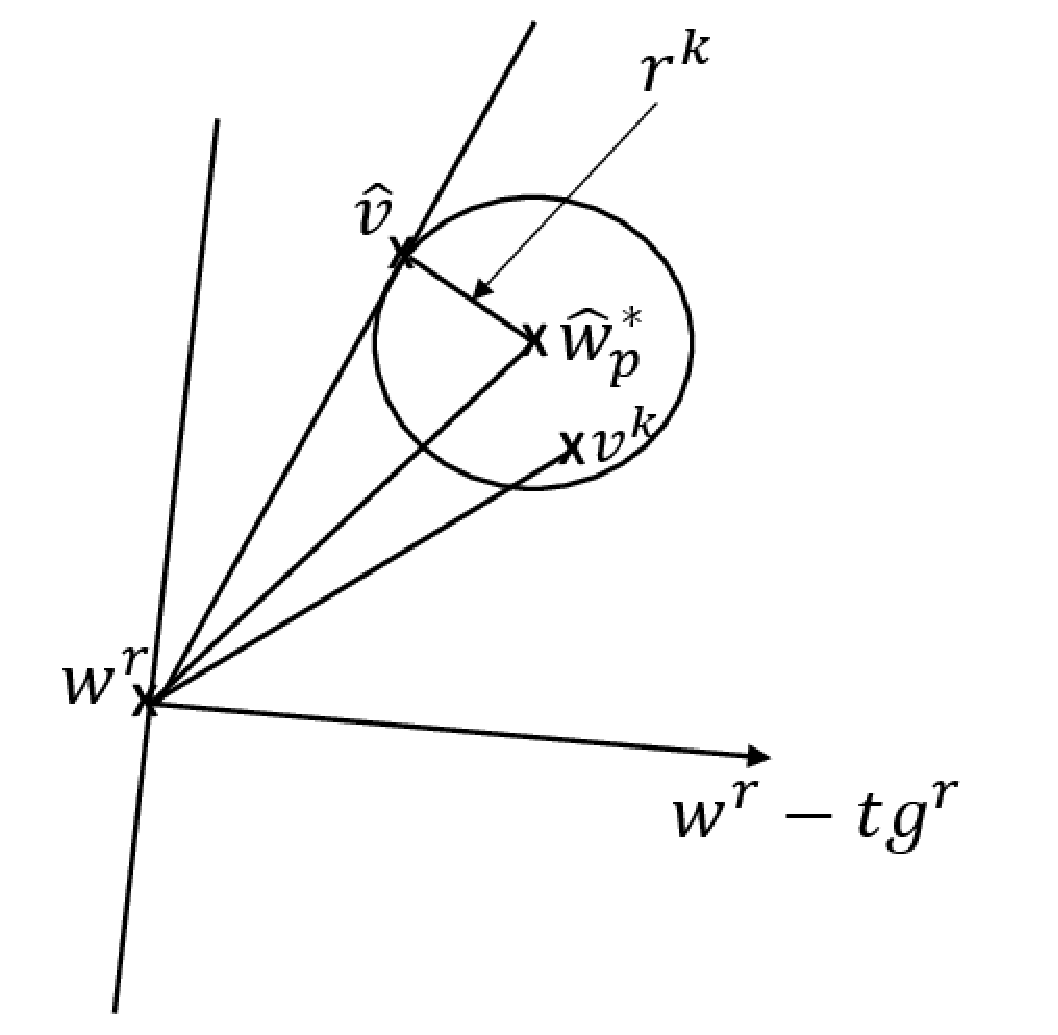
\includegraphics[width=0.6\columnwidth]{spherefig}
\caption{Construction used in the proof of Lemma 3.}
\end{center}
\label{spherefig}
\end{figure}


By A3 and equations ($3.16$) and ($3.22$) in~\cite{smola2008}, we get
\begin{equation}
\frac{\sigma}{2} \|v-\what_p^\star\|^2 \le \fhat_p(v) - \fhat_p^\star \le \frac{L}{2} \|v-\what_p^\star\|^2
\label{lem221}
\end{equation}
After $k$ iterations we have
\begin{equation}
\fhat_p(v^k) - \fhat_p^\star \le \delta^k (\fhat_p(w^r) - \fhat_p^\star)
\label{lem222}
\end{equation}
We can use these to get
\begin{eqnarray}
\|v^k-\what_p^\star\|^2 \le \frac{2(\fhat_p(v^k)-\fhat_p^\star)}{\sigma}
                        \le \frac{2\delta^k (\fhat_p(w^r)-\fhat_p^\star)}{\sigma}
                        \le \frac{\delta^kL}{\sigma} \|w^r-\what_p^\star\|^2 \defs (r^k)^2
\label{lem223}
\end{eqnarray}
For now let us assume the following:
\begin{equation}
\|v^k-\what_p^\star\|^2 \le \|w^r-\what_p^\star\|^2
\label{lem224}
\end{equation}
Using (\ref{lem223}) note that (\ref{lem224}) holds if
\begin{equation}
\frac{\delta^kL}{\sigma} \le 1
\label{lem225}
\end{equation}
Let $S^k$ be the sphere, $S^k = \{ v : \|v-\what_p^\star\|^2 \le (r^k)^2 \}$. By (\ref{lem223})
%and (\ref{lem224})
we have $v^k\in S^k$. See Figure~\ref{spherefig}. Therefore,
\begin{equation}
\phi^k \le \max_{v\in S^k} \phi(v)
\label{lem226}
\end{equation}
where $\phi^k$ is the angle between $\what_p^\star-w^r$ and $v^k-w^r$, and $\phi(v)$ is the angle between $v-w^r$ and $\what_p^\star-w^r$. Given the simple geometry, it is easy to see that $\max_{v\in S^k} \phi(v)$ is attained by a point $\vhat$ lying on the boundary of $S^k$ (i.e., $\|\vhat-\what_p^\star\|^2 = (r^k)^2$) and satisfying $(\vhat-\what_p^\star)\perp (\vhat-w^r)$. This geometry yields
\begin{eqnarray}
\cos^2 \phi(\vhat) = \frac{\|\vhat-w^r\|^2}{\|\what_p^\star-w^r\|^2}
                   = \frac{\|\what_p^\star-w^r\|^2-(r^k)^2}{\|\what_p^\star-w^r\|^2}
                   = 1-\frac{(r^k)^2}{\|\what_p^\star-w^r\|^2} = 1-\frac{\delta^kL}{\sigma}
\label{lem227}
\end{eqnarray}
Since $\phi^k\le \phi(\vhat)$,
\begin{equation}
\cos^2 \phi^k \ge 1-\frac{\delta^kL}{\sigma}
\label{lem228}
\end{equation}
Thus, if
\begin{equation}
1-\frac{\delta^kL}{\sigma} \ge \zeta^2
\label{lem229}
\end{equation}
then
\begin{equation}
\cos \phi^k \ge \zeta \;\; \forall k\ge \khat
\label{22b}
\end{equation}
holds. By (\ref{lem2211}) this yields $\phase{-g^r,v^k-w^r} \le \theta$, the result needed in Lemma 3. Since $\zeta>0$, (\ref{lem229}) implies (\ref{lem225}), so (\ref{lem224}) holds and there is no need to separately satisfy it. Now (\ref{lem229}) holds if
\begin{equation}
k \ge \khat \defs \frac{\log (L/(\sigma(1-\zeta^2)))}{\log(1/\delta)}
\label{lem2210}
\end{equation}
which proves the lemma.

\vspace*{0.1in}

\noindent{\bf Proof of Theorem 4.} It trivially follows from a combination of Lemma 3 and Theorem 2.

%
% The following two commands are all you need in the
% initial runs of your .tex file to
% produce the bibliography for the citations in your paper.
%\bibliographystyle{plain}
\bibliography{15-020}  % sigproc.bib is the name of the Bibliography in this case
% You must have a proper ".bib" file
%  and remember to run:
% latex bibtex latex latex
% to resolve all references
%
% ACM needs 'a single self-contained file'!
%


\end{document}
